\documentclass[conference]{IEEEtran}
\IEEEoverridecommandlockouts
% The preceding line is only needed to identify funding in the first footnote. If that is unneeded, please comment it out.
\usepackage{cite}
\usepackage{amsmath,amssymb,amsfonts}
\usepackage{algorithmic}
\usepackage{graphicx}
\usepackage{textcomp}
\usepackage{diagbox}
\usepackage{subfigure}
\usepackage{xcolor}
\def\BibTeX{{\rm B\kern-.05em{\sc i\kern-.025em b}\kern-.08em
    T\kern-.1667em\lower.7ex\hbox{E}\kern-.125emX}}
\begin{document}

\title{Domain Adaptation for Image Classification\\
%{\footnotesize \textsuperscript{*}Note: Sub-titles are not captured in Xplore and
%should not be used}
%\thanks{Identify applicable funding agency here. If none, delete this.}
}

\author{\IEEEauthorblockN{Haowei Huang}
\IEEEauthorblockA{\textit{516021910491} \\
\textit{Shanghai Jiao Tong University}\\
Shanghai, China \\
1270927224@qq.com}
\and
\IEEEauthorblockN{Zhixin Lin}
\IEEEauthorblockA{\textit{516021910495} \\
\textit{Shanghai Jiao Tong University}\\
Shanghai, China \\
1069066484@qq.com}
\and
\IEEEauthorblockN{Yaojie Ding}
\IEEEauthorblockA{\textit{516021910430} \\
\textit{Shanghai Jiao Tong University}\\
Shanghai, China \\
416914846@qq.com}
}

\maketitle

\begin{abstract}
We use four traditional methods, TCA, CORAL, KMM and JDA, and three deep methods, DaNN, ADDA and DANN of domain adaptation on deep features of OfficeHome-Dataset. And the performances of these methods are compared. We find all of the seven approaches can work in some degree. Accuracies improve by 0.03 at most with these methods. And, deep methods, which show many advantages over traditional methods in machine learning, though, do not obviously overcome traditional methods in the work of domain adaptation.
\end{abstract}



\section{Introduction}
Currently, many classification approaches are assuming that training samples and test samples are subject to the same distribution. But there can always be probability distribution mismatch between the training and test samples. For example, we collect training images with our smart phones to train an object recognizer and apply the trained model to a unmanned aerial vehicle. Therefore, we need to solve the distribution mismatch to make the object recognizer applicable in the aerial view. A model that is able to adapt to different environments is more robust and reliable. And domain adaptation is a class of methods to solve the problem.

In our work, we use seven methods of domain adaptation on deep features of OfficeHome-Dataset and summarize differences and similarities of these approaches' theories and performances. We investigate whether and how the domain adaptation methods can work to solve mismatch of different data distributions.
\section{Approaches}
In this section, we have two parts to elaborate traditional and deep methods applied for domain adaptation. We don't repeat too much common descriptions but emphasize our differences.

\subsection{Traditional Methods}
\subsubsection{TCA}
Pan, Sinno Jialin, et al. proposed to find a representation through a learning method, transfer component analysis(TCA), for domain adaptation in \cite{TCA}. TCA tries to learn a set of common transfer components underlying both domains such that the difference in data distributions of the different domains, when projected onto this subspace, can be dramatically reduced and data properties can be preserved.

Mathematically, TCA aim to minimize the difference
\begin{equation}
    \begin{aligned}
      d(W^TX_s,& W^TX_t)^2 =   \\
            &||\frac{1}{n_s} \sum\limits_{i=1}^{n_s} \phi(W^TX_{s,i}) - \frac{1}{n_t} \sum\limits_{i=1}^{n_t} \phi(W^TX_{t,i})||^2
    \end{aligned}
\end{equation}
where $W^T$ is a projection matrix, $X_s$ the source data, $X_t$ the target data, $n_s$ number of source samples, $n_t$ number of target samples, and $\phi$ a complicated transformation represented using kernel trick when solving the optimization. The difference is squared MMD(maximum mean discrepancy) after projected with $W^T$. MMD is usually used as a measurement of difference between two distribution.

\subsubsection{CORAL}
Sun, Baochen, Jiashi Feng, and Kate Saenko proposed a simple, effective, and efficient method for unsupervised domain adaptation called CORrelation ALignment(CORAL) in \cite{CORAL}. CORAL minimizes domain shift by aligning the second-order statistics of source and target distributions, without requiring any target labels.

Mathematically, CORAL aims to find an $X_s$'s projection matrix $A$ to minimize the difference between covariances of $X_t$ and projected $X_s$:
\begin{equation}
J(A) = ||A^TC_sA-C_t||_F^2
\end{equation}
where $C_s$ and $C_t$ are respectively covariance of $X_s$ and $X_t$. Frobenius norm is used to evaluate the covariance difference.

\subsubsection{KMM}
Huang, Jiayuan, et al. presented a nonparametric method which directly produces resampling weights without distribution estimation to deal with data adaptation in \cite{KMM}. Their method is called kernel mean matching(KMM), which works by matching distributions between training and testing sets in feature space.
\begin{figure}
  \centering
  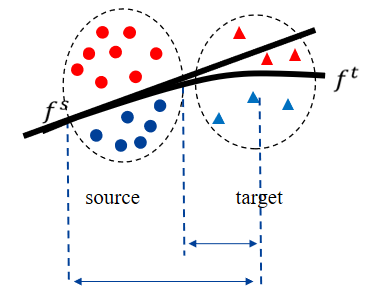
\includegraphics[width=.4\textwidth]{LKMM_theorem1.png}
  \caption{Theory of KMM}
  \label{KMM_theorem}
\end{figure}
The idea of KMM is sophisticated. As illustrated in figure \ref{KMM_theorem}, it just like assigning different weights for different source samples when training SVM. This is equivalently minimizing distance of source and target centers.
Mathematically, before training SVM, KMM finds a $\beta_i$ for each source sample $X_{s,i}$ to minimize
\begin{equation}
d(X_s, X_t)^2 = ||\frac{1}{n_s} \sum\limits_{i=1}^{n_s}\beta_i \phi(X_{s,i}) - \frac{1}{n_t} \sum\limits_{i=1}^{n_t} \phi(X_{t,i}) ||^2
\end{equation}
The optimization target is also MMD. After that, $\beta_i$ is used as a multiplier for slack variable in SVM's optimization target $\frac{1}{2}||w||^2+C\sum\limits_{i}\beta_i \xi_i$.

\subsubsection{JDA}
Mingsheng Long, et al. put forward a novel transfer learning approach, referred to as Joint Distribution Adaptation(JDA) in \cite{JDA}. Specifically, JDA aims to jointly adapt both the marginal distribution and conditional distribution in a principled dimensionality reduction procedure, and construct new feature representation that is effective and robust for substantial distribution difference.

Using a high-level mathematical description, JDA tries to find a feature transformation $T$ minimize difference of joint distributions of source and target data:
\begin{equation}
J(T) = || \mathbb{E}_{P(X_s,y_s)}[T(X_s), y_s] - \mathbb{E}_{P(X_t,y_t)}[T(X_t), y_t]||^2
\end{equation}
Since $y_t$ is assumed to be unknown, Mingsheng Long, et al. used some approximation for the optimization.

\subsection{Deep Methods}
\subsubsection{DaNN}
Muhammad Ghifary, et al. propose a simple neural network model to deal with the domain adaptation problem in \cite{DaNN}. This model incorporates the Maximum Mean Discrepancy(MMD) measure as a regularization in the supervised learning to reduce the distribution mismatch between the source and target domains in the latent space. This model is called Domain Adaptive Neural Network(DaNN), which in fact is a variant of the standard feed forward neural network.

The way this model runs can be described as follows:
\begin{enumerate}
\item Calculate the loss function. Given the labeled source data $\left\{\mathbf{X}_{s}^{(i)}, \mathbf{y}_{s}^{(i)}\right\}_{i=1, \ldots, n_{s}}$ and the unlabeled target data $\left\{\mathbf{x}_{t}^{(j)}\right\}_{j}=1, \ldots, n_{t}$, the loss function of a single layer DaNN is given by
\begin{equation}
J_{\mathrm{DaNN}}=J_{\mathrm{NNs}}+\gamma \mathcal{M M D}_{e}^{2}\left(\mathrm{q}_{s}, \overline{\mathrm{q}}_{t}\right)
\end{equation}
where \\
$J_{\mathrm{NNS}}=-\frac{1}{n_{s}} \sum_{i=1}^{n_{s}} \sum_{k=1}^{l}\left(\left[\mathbf{y}_{s}^{(i)}\right]_{k} \log \left(\left[f\left(\mathbf{x}_{s}^{(i)}\right)\right]_{k}\right)\right)$, $\mathbf{q}_{s}=\mathbf{W}_{1}^{\top} \mathbf{x}_{s}+\mathbf{b}$, $\overline{\mathrm{q}}_{t}= \mathbf{W}_{1}^{\top} \mathbf{x}_{t}+\mathbf{b}$ are the linear combination outputs before the activation,and $\gamma$ is the regularization constant controlling the importance of MMD contribution to the loss function.\\
\item Minimize the loss function. We choose the Gaussian kernel as the kernel function of the form $k_{G}(\mathrm{x}, \mathrm{y})=\exp \left(-\frac{\|\mathrm{x}-\mathrm{y}\|^{2}}{2 s^{2}}\right)$, where $s$ is the standard deviation and rewrite $\mathcal{M} \mathcal{M} \mathcal{D}_{e}^{2}(\cdot, \cdot)$ as:
\begin{tiny}
\begin{eqnarray}
\begin{aligned}
\mathcal{M M D}_{e}^{2}&\left(\mathbf{U}_{1}^{\top} \mathbf{X}_{s}, \mathbf{U}_{1}^{\top} \mathbf{X}_{t}\right)= \\
& \frac{1}{n_{s}^{2}} \sum_{i, j=1}^{n_{s}} \exp \left(-\frac{\left(\mathbf{x}_{s}^{(i)}-\mathbf{x}_{s}^{(j)}\right)^{\top} \mathbf{U}_{1} \mathbf{U}_{1}^{\top}\left(\mathbf{x}_{s}^{(i)}-\mathbf{x}_{s}^{(i)}\right)}{2 s^{2}}\right)\\
& +\frac{1}{n_{t}^{2}} \sum_{i, j=1}^{n_{t}} \exp \left(-\frac{\left(\mathrm{x}_{t}^{(i)}-\mathrm{x}_{t}^{(j)}\right)^{\top} \mathrm{U}_{1} \mathbf{U}_{1}^{\top}\left(\mathrm{x}_{t}^{(i)}-\mathrm{x}_{t}^{(i)}\right)}{2 s^{2}}\right)\\
& -\frac{2}{n_{s} n_{t}} \sum_{i, j=1}^{n_{s}, n_{t}} \exp \left(-\frac{\left(\mathbf{x}_{s}^{(i)}-\mathbf{x}_{t}^{(j)}\right)^{\top} \mathbf{U}_{1} \mathbf{U}_{1}^{\top}\left(\mathbf{x}_{s}^{(i)}-\mathbf{x}_{t}^{(i)}\right)}{2 s^{2}}\right)
\end{aligned}
\end{eqnarray}
\end{tiny}
In the implementation, we separate the minimization of $J_{\mathrm{NNs}}$ and $\mathcal{M} \mathcal{M} \mathcal{D}_{e}^{2}(\cdot, \cdot)$ into two step. Firstly, $J_{\mathrm{NNs}}$ is minimized using a $mini-batched$ stochastic gradient descent with respect to $\mathbf{U}_{1}$ update. Then, $\mathcal{M} \mathcal{M} \mathcal{D}_{e}^{2}(\cdot, \cdot)$ is minimized by re-updating $\mathbf{U}_{1}$. The latter step is accomplished by a full-batched
gradient descent.
\end{enumerate}
DaNN is rather a simple neural network(with only 1 hidden layer) for domain adaptation. But its idea is important that brings MMD(maximum mean discrpancy) for adaptation in neural network.

\subsubsection{ADDA}
Eric Tzeng, et al. summarized a generalized architecture for adversarial domain adaptation and introduced a method of domain adaptation, Adversarial Discriminative Domain Adaptation, in his work \cite{ADDA1}. Using their summary, ADDA is a combination of generative and discriminative neural network model that uses untied weight sharing between source mapping and target mapping and a GAN loss.

\begin{figure*}
  \centering
  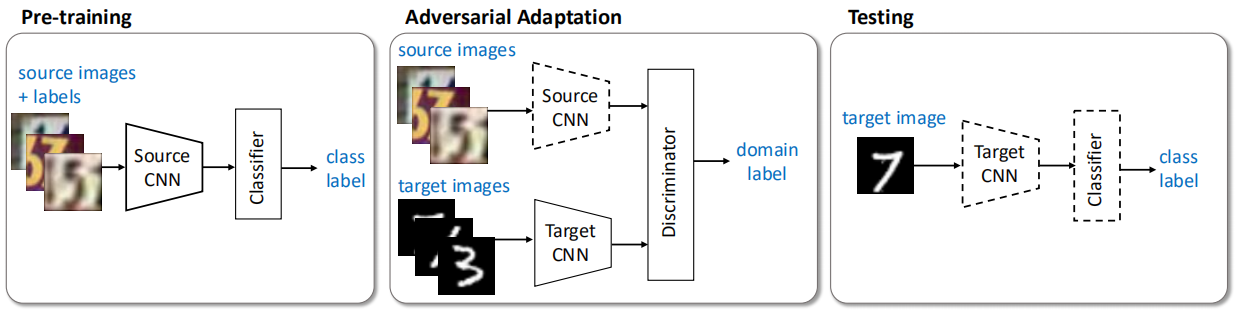
\includegraphics[width=.75\textwidth]{LADDA_theorem1.jpg}
  \caption{ADDA Overview: An overview of standard ADDA architecture. Dashed lines indicate fixed network parameters in the indicated stage.}
  \label{ADDA_overview}
\end{figure*}
The general ADDA approach is presented in figure \ref{ADDA_overview}. There are overall four relatively separated subnetworks within the ADDA model:
\begin{enumerate}
  \item Source encoder network, $M_s$. Source encoder take source data set as input and output the encoded source features.
  \item Target encoder network, $M_t$. Target encoder take source data set as input and output the encoded target features.
  \item Discriminator network, $D$. Discriminator take encoded source features and encoded target features and tries to identify which come from source dataset and target dataset.
  \item Classifier network, $C$. Classifier network take encoded features, from either source or target domain, as input and output the class prediction.
\end{enumerate}

According to work of Eric Tzeng, et al., we can divide the way the model runs into three stages:
\begin{enumerate}
  \item Pre-training. In this stage, we feed source training data, $X_{s}$ for source encoder network and use the output features, $M_s(X_{s})$, to feed classifier network and use cross entropy as classification loss , $L_{c}$:
      \begin{equation}\label{cls_loss}
      \begin{aligned}
        L_{c} & (X_{s}, Y_{s}) =  \\
        &-\mathbb{E}_{(x_s,y_s) \sim (X_s,Y_s)}
        \sum\limits_{k=1}^{K} \mathbb{I}_{[k=y_s]} \log C(M_s(X_{s}))
        \end{aligned}
      \end{equation}
       to train the source network and classifier network. After that, both source network and classifier network are fixed. $K$ is the total number of classes.
  \item Adversarial adaptation. In this stage, we use the idea of GAN to train $M_t$ to generate features, $M_t(X_{t})$, to be similarly distributed as $M_s(X_{s})$. We feed $X_s$ and $X_t$ for $M_s$ and $M_t$ respectively and combination of $M_s(X_{s})$ and $M_t(X_{t})$ for $D$. We in turn optimize $D$ to minimize $L_{D}$:
      \begin{equation}\label{LD}
        \begin{aligned}
        L_{D} & (X_{s}, X_{t}, M_s, M_t) =  \\
                                        &-\mathbb{E}_{(x_s) \sim (X_s)} \log D(M_s(X_{s})) \\
                                        &-\mathbb{E}_{(x_t) \sim (X_t)} \log (1 - D(M_t(X_{t}))
            \end{aligned}
      \end{equation}
      and optimize $M_t$ to minimize
      $L_{t}$:
      \begin{equation}\label{Lt}
        L_{t}(X_{s}, X_{t}, D) =
            -\mathbb{E}_{(x_t) \sim (X_t)} \log D(M_t(X_{t}))
      \end{equation}
      $D$ tries to distinguish $M_s(X_{s})$ and $M_t(X_{t})$ while $M_t$ want to deceive $D$. \\
      Our approach is not always quite standard as Eric Tzeng's work. Except that we use fully connected layers instead of CNN for our $X_s$ and $X_t$, we also initialized parameters of $M_t$ using pre-trained $M_s$'s. This is not mentioned in the paper and it is not likely to be feasible in most cases. We can do so because our structure of $M_s$ is designed to be the same as $M_t$. And the measure really help a lot.
  \item Testing. In this stage, we feed $M_t(X_t)$ for $C$ and evaluate the classification accuracy.
\end{enumerate}
    In practice, we combined the last two stages into one, just say adversarial adaptation. ADDA method is just like trying to encode the target domain data, $M_t(X_t)$, to match the distribution of encoded source domain data, $M_s(X_s)$ so that the classifier working on source domain data can also work on target domain data.




\subsubsection{DANN}
Yaroslav Ganin, et al. proposed a representation learning approach for domain adaptation in their work \cite{DANN1}. DANN can also be viewed as an instance of Eric Tzeng, et al.'s summary of domain adaptation method. Compared with ADDA, in general, the only difference of DANN is that DANN is an architecture of tied weight sharing.
\begin{figure*}
  \centering
  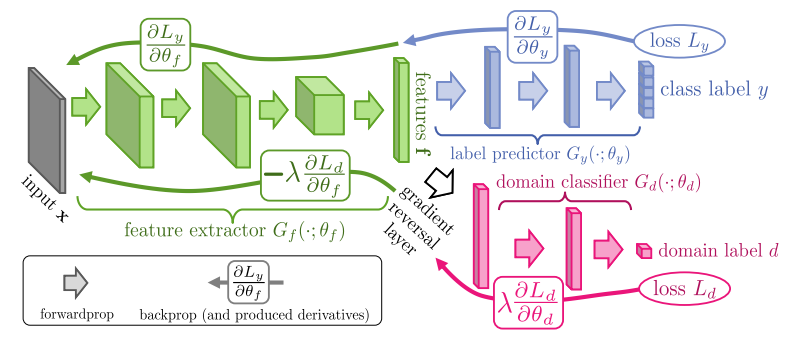
\includegraphics[width=.8\textwidth]{LDANN_theorem1.jpg}
  \caption{DANN Overview: An overview of standard DANN architecture.}
  \label{DANN_overview}
\end{figure*}
The general architecture is presented in figure \ref{DANN_overview}; it's simpler than ADDA. Domain classifier $D$ of DANN performs similar function as discriminator $D$ of ADDA does. DANN is similar to ADDA but target encoder and source encoder share the same weight weights. In other words, only one feature encoder, $M$, is used within DANN. Thus, we do not go to details of components of DANN and just simply present the way the DANN model work. We will use similar representations as ADDA to make things easy to understand (although they may not be Yaroslav Ganin et al.'s symbols).
\begin{enumerate}
  \item Pre-training. In this stage, we optimize $M$ and $C$ to minimize $L_{C}$.
  \item Adversarial adaptation. In this stage, we feed both $X_s$ and $X_t$ for $M$. By fixing $C$, we optimize $M$ and $D$ to minimize $L_{da}$:
      \begin{equation}\label{dann_da}
        \begin{aligned}
        L_{da} & (X_{s}, X_{t}, M) =  \\
                            &-(\mathbb{E}_{(x_s) \sim (X_s)} \log D(M(X_{s})) \\
                            &+\mathbb{E}_{(x_t) \sim (X_t)} \log (1 - D(M(X_{t}))) \times c_{da} \\
                            &-\mathbb{E}_{(x_s,y_s) \sim (X_s,Y_s)}
                            \sum\limits_{k=1}^{K} \mathbb{I}_{[k=y_s]} \log C(M(X_{s}))
        \end{aligned}
      \end{equation}
      Unlike ADDA, parameters of $M$ and $D$ are updated at the same time. And the loss, $L_{da}$ of DANN is combination of both $L_C$ and $L_D$ of ADDA. There is subtle difference between ADDA and DANN in this stage. $C_{da}$ is a balance factor for classification loss and discriminator loss. $c_{da}$ is not mentioned in the paper, but we use it and find it helps improve our model. We use $c_{da}=2.0$.
  \item Testing. In this stage, we feed $M(X_t)$ for $C$ and evaluate the classification accuracy.
\end{enumerate}
Also, we combined stage of adversarial adaptation and testing together as adversarial adaptation. Compared to ADDA method that tries to bring $M_t(X_t)$ to $M_s(X_s)$ as closer as possible, DANN method is just like trying to adjust a well-trained source domain encoder $M_s$ to work on target domain data, $X_t$.

\section{Experiments And Results}
In this section, we have three parts to present experiments of traditional methods, experiments of deep methods and a summary respectively.

\subsection{Traditional Methods}
In this section we will show the experiments that we have done by using traditional domain adaptation methods.
First of all, in Table~\ref{tab:RAW}, we will show the test accuracy of some classification methods on target domain if we do not any apply domain adaptation method. These can be treated as baselines. In this part, we train the classifiers on source domain and test them on target domain. 1NN means k-NN method with $k=1$. In this section, we use $X_s$, $X_t$, $X_t\_new$, $X_s\_new$ respectively to denote the features of source domain, the features of target domain, the features of source domain which has been reconstructed by domain adaptation method and the features of target domain which has been reconstructed by domain adaptation method. We use $A2R$ to show the source domain is Art and the target domain is RealWorld. $C2R$ and $P2R$ are similar to $A2R$. And $SVM\_lin$ means SVM with linear kernel while $SVM\_RBF$ means SVM with RBF kernel.

 \begin{table}[h]
 \begin{scriptsize}
	\centering
	\caption{testing accuracy without domain adaptation method}
	\label{tab:RAW}
	\begin{tabular}{cccccc}
		\hline
		Src &Tar&KNN&SVM(linear)&SVM(RBF,C=1)&SVM(RBF,C=5) \\
		\hline
		\hline
        $Art$ & $Real$ & 0.6580 & 0.7310 & 0.7436 & 0.7473 \\
		$Clipart$ & $Real$ & 0.5864& 0.6013 & 0.6488 & 0.6511\\
		$Product$ & $Real$ & 0.6957& 0.6879 & 0.7266 & 0.7296  \\
		\hline
	\end{tabular}
\end{scriptsize}
\end{table}

\subsubsection{TCA Experiments}
In this section we have done three parts of experiments. The experiments of the first two parts have been shown in Table~\ref{tab:TCA1}, Table~\ref{tab:TCA2} and Table~\ref{tab:TCA3}
\begin{table}[h]
\begin{tiny}
\centering
	\caption{A2R: part1 and part2 }
	\begin{tabular}{c|c|c|c|c|c|c|c}
	\label{tab:TCA1}\\
	\hline
	\diagbox{classifier}{testing accuracy}{dim} & 32 & 64 & 128 & 256 & 512 &1024 &2048 \\
	\hline
	$SVM\_lin$ &0.7067&0.7434&0.7540&0.7563&0.7572&0.7567&0.7567\\
	\hline
	$SVM\_RBF(C=1)$ &0.7122 &0.7418&0.7519&0.7466&0.7464&0.7448&0.7434\\
	\hline
	$SVM\_RBF(C=5)$ &0.7207&0.7519&0.7590&0.7599&0.7604&0.7602&0.7602\\
	\hline
	\end{tabular}
\end{tiny}
\end{table}

\begin{table}[h]
\begin{tiny}
\centering
	\caption{C2R: part1 and part2 }
	\begin{tabular}{c|c|c|c|c|c|c|c}
	\label{tab:TCA2}\\
	\hline
	\diagbox{classifier}{testing accuracy}{dim} & 32 & 64 & 128 & 256 & 512 &1024 &2048 \\
	\hline
	$SVM\_lin$ &0.6282&0.6523&0.6612&0.6677&0.6688&0.6695&0.6693\\
	\hline
	$SVM\_RBF(C=1)$ &0.6440&0.6553&0.6550&0.6543&0.6530&0.6527&0.6530\\
	\hline
	$SVM\_RBF(C=5)$ &0.6369&0.6534&0.6587&0.6562&0.6557&0.6562&0.6553\\
	\hline
	\end{tabular}
\end{tiny}
\end{table}

\begin{table}[h]
\begin{tiny}
\centering
	\caption{P2R: part1 and part2 }
	\begin{tabular}{c|c|c|c|c|c|c|c}
	\label{tab:TCA3}\\
	\hline
	\diagbox{classifier}{testing accuracy}{dim} & 32 & 64 & 128 & 256 & 512 &1024 &2048 \\
	\hline
	$SVM\_lin$ &0.7101&0.7287&0.7354&0.7377&0.7404&0.7406&0.7402\\
	\hline
	$SVM\_RBF(C=1)$ &0.7248&0.7429&0.7372&0.7393&0.7395&0.7395&0.7393\\
	\hline
	$SVM\_RBF(C=5)$ &0.7131&0.7310&0.7296&0.7305&0.7305&0.7310&0.7308\\
	\hline
	\end{tabular}
\end{tiny}
\end{table}

In these two parts we have set the kernel method TCA uses to be 'primal' which means TCA does not apply kernel method.

The first part is about different dimensions of features of source domain and target domain after TCA process. From the three tables above, we can find a interesting phenomenon that with the number of dimensions growing, all the testing accuracy of different classifier and different combination of source domain and target domain initially goes higher but stays stable when dimensions have reach 512. We guess the reason is that with the reconstruction of TCA, when $X_s\_new$' dimensions reach 512, $X_s\_new$ and $X_t\_new$ contains enough information. The Maximum Mean Discrepancy becomes small between source domain and target domain and different domains are close to each other and testing accuracy reach a high point.

The second part is about different classifiers. We can find for all $A2R$, $C2R$ and $P2R$, when the number of dimensions is small, $SVM\_RBF$ performs better than $SVM\_lin$ while the case is the contrary when dimensions is bigger. This is because $SVM\_lin$ is suitable for the situation that number of features and number of samples are close and $SVM\_RBF$ is suitable for the situation that the number of features is small. And for the hyper-parameter $C$ in $SVM\_RBF$, we find a bigger $C$ can performs better on $A2R$ and $C2R$ but a small $C$ is better on $P2R$.

Then we show the result of the third part in Table~\ref{tab:TCA4}, Table~\ref{tab:TCA5} and Table~\ref{tab:TCA6}.
\begin{table}[h]
\begin{scriptsize}
\centering
	\caption{A2R: part3}
	\begin{tabular}{c|c|c|c}
	\label{tab:TCA4}\\
	\hline
	\diagbox{classifier}{testing accuracy}{TCA kernel type} & primal & linear & RBF \\
	\hline
	$SVM\_lin$ &0.7567&0.4983&0.5554\\
	\hline
	$SVM\_RBF$ &0.7434&0.1958&0.0.2454\\
	\hline
	\end{tabular}
\end{scriptsize}
\end{table}

\begin{table}[h]
\begin{scriptsize}
\centering
	\caption{C2R: part3}
	\begin{tabular}{c|c|c|c}
	\label{tab:TCA5}\\
	\hline
	\diagbox{classifier}{testing accuracy}{TCA kernel type} & primal & linear & RBF \\
	\hline
	$SVM\_lin$ &0.6693&0.5625&0.5965\\
	\hline
	$SVM\_RBF$ &0.6530&0.3002&0.3514\\
	\hline
	\end{tabular}
\end{scriptsize}
\end{table}

\begin{table}[h]
\begin{scriptsize}
\centering
	\caption{P2R: part3}
	\begin{tabular}{c|c|c|c}
	\label{tab:TCA6}\\
	\hline
	\diagbox{classifier}{testing accuracy}{TCA kernel type} & primal & linear & RBF \\
	\hline
	$SVM\_lin$ &0.7402&0.6635&0.6945\\
	\hline
	$SVM\_RBF$ &0.7393&0.5280&0.5843\\
	\hline
	\end{tabular}
\end{scriptsize}
\end{table}
For this part we have set dimensions to be 2048 and try to find the difference between different kernel method in TCA. From Table~\ref{tab:TCA4} we can find that we get rather bad results with TCA(RBF) and TCA(linear). Besides, in the experimental process, the run time of TCA(RBF) and TCA(linear) is very long.

\subsubsection{CORAL Experiments}
As Baochen Sun, et al. has pointed in \cite{CORAL}, CORAL is a "frustratingly easy" domain adaptation method which does not have many parameters. So in this section, we have compared the performances of CORAL on different source-target combinations and different classifier.
\begin{table}[h]
\begin{tiny}
\centering
	\caption{CORAL experiments}
	\begin{tabular}{c|c|c|c|c}
	\label{tab:CORAL}\\
	\hline
	\diagbox{Src\&Tar}{testing accuracy}{classifier} & KNN & SVM\_lin & SVM\_RBF(C=1) & SVM\_RBF(C=5) \\
	\hline
	$A2R$ &0.6488&0.7090&0.7390&0.7450\\
	\hline
	$C2R$ &0.5830&0.5997&0.6514&0.6504\\
	\hline
	$P2R$ &0.6851&0.6906&0.7310&0.7276\\
	\hline
	\end{tabular}
\end{tiny}
\end{table}
From Table~\ref{tab:CORAL} we can find $SVM\_RBF$ performs much better than $1NN$ and $SVM_lin$. The change of hyper-parameter $C$ does not have a big influence on the performance. And we can compare the performance of CORAL with results that have been shown in Table~\ref{tab:RAW}. The performance of CORAL is even worse than the situation without domain adaptation method. This may be the price of "frustrating easy".

\subsubsection{KMM Experiments}
In this section, we have change the kernel type that KMM uses to see the different performance of KMM. Of course we have tried different classifier and apply them on different source domain and target domain.
\begin{table}[h]
%\begin{tiny}
\centering
	\caption{KMM experiments on $A2R$}
	\begin{tabular}{c|c|c}
	\label{tab:KMM1}\\
	\hline
	\diagbox{classifier}{testing accuracy}{kernel type} & linear & RBF \\
	\hline
	$SVM\_lin$ &0.7296&0.7312\\
	\hline
	$SVM\_RBF(C=1)$ &0.6729 &0.7356\\
	\hline
	$SVM\_RBF(C=5)$ &0.6723&0.7471\\
	\hline
	\end{tabular}
%\end{tiny}
\end{table}

\begin{table}[h]
%\begin{tiny}
\centering
	\caption{KMM experiments on $C2R$}
	\begin{tabular}{c|c|c}
	\label{tab:KMM2}\\
	\hline
	\diagbox{classifier}{testing accuracy}{kernel type} & linear & RBF \\
	\hline
	$SVM\_lin$ &0.6004&0.5143\\
	\hline
	$SVM\_RBF(C=1)$ &0.5974 &0.6518\\
	\hline
	$SVM\_RBF(C=5)$ &0.5116&0.6518\\
	\hline
	\end{tabular}
%\end{tiny}
\end{table}

\begin{table}[h]
%\begin{tiny}
\centering
	\caption{KMM experiments on $P2R$}
	\begin{tabular}{c|c|c}
	\label{tab:KMM3}\\
	\hline
	\diagbox{classifier}{testing accuracy}{kernel type} & linear & RBF \\
	\hline
	$SVM\_lin$ &0.6876&0.6927\\
	\hline
	$SVM\_RBF(C=1)$ &0.6617 &0.7299\\
	\hline
	$SVM\_RBF(C=5)$ &0.6633&0.7273\\
	\hline
	\end{tabular}
%\end{tiny}
\end{table}

From Table~\ref{tab:KMM1}, Table~\ref{tab:KMM2} and Table~\ref{tab:KMM3} we can find when  KMM uses linear kernel, $SVM\_lin$ performs better than $SVM\_RBF$. When KMM uses RBF kernel, the case is the contrary. We conclude that the kernel method used in KMM and the kernel method used in SVM should be consistent.

\subsubsection{JDA Experiments}
In this part we will show performances of JDA with different dimensions after transfer. In this experiment, we use $SVM_RBF$ as classifier and the hyper-parameter $C$ of SVM is 1.
\begin{table}[h]
\begin{tiny}
\centering
	\caption{JDA experiments}
	\begin{tabular}{c|c|c|c|c|c|c|c}
	\label{tab:JDA}\\
	\hline
	\diagbox{Src\&Tar}{testing accuracy}{dim} & 32 & 64 & 128 & 256 & 512 &1024 &2048 \\
	\hline
	$A2R$ &0.7092&0.7462&0.7530&0.7471&0.7464&0.7464&0.7457\\
	\hline
	$C2R$ &0.6543&0.6638&0.6656&0.6628&0.6601&0.6605&0.6608\\
	\hline
	$P2R$ &0.7351&0.7459&0.7436&0.7471&0.7482&0.7478&0.7478\\
	\hline
	\end{tabular}
\end{tiny}
\end{table}
Similar to the results of TCA, with the increase of dimensions, the testing accuracy initially increase and then reach the highest point. Finally the testing accuracy stay stable. This similarity can be explained by the fact that TCA and JDA both use Maximum Mean
Discrepancy (MMD) to measure the difference between the distribution of source domain and the distribution of target domain.

\subsection{Deep Methods}
\subsubsection{DaNN Experiments}
We will present five parts of experiments in this section to evaluate the influence of different parameter in this model. Since DaNN is rather a simple neural network with only 1 hidden layer for domain adaptation, there are not many details of building this network. In the all five parts of experiments, we set $Learning\_rate = 0.05$, $Epochs = 30$. For each combination of source domain and target domain, we use the data in source domain to be the training set and the data in target domain to be the testing set. Besides, in this section we use $\lambda$ to denote the coefficient of mmd\_loss in the calculation of total loss, $DR$ to denote the drop rate and $BS$ to denote the batch size.

For the first part, we show the change of training accuracy, testing accuracy, training loss and testing loss during the running process of this network. All values of the loss curves are scaled to interval $[0.0, 1.0]$ for a better observation. For this part, we have set $\lambda = 1$, $DR = 0.5$, $BS = 64$. The combination of target domain and source domain we choose is $P2R$. Figure~\ref{fig:DaNN1} shows the result.
\begin{figure}[!h]
    \centerline{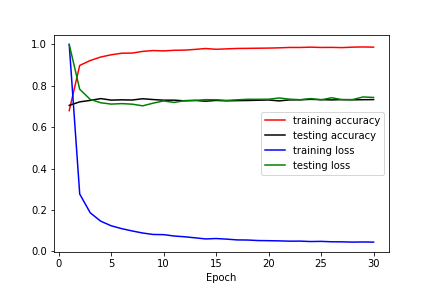
\includegraphics[scale=0.4]{HDaNN/DaNN_fig1.png}}
    \caption{DaNN: part 1}
    \label{fig:DaNN1}
\end{figure}

From figure~\ref{fig:DaNN1} we can find both training accuracy and testing accuracy have a quick convergence. However, there exists a problem that though training accuracy and training loss have a nice trend, the testing accuracy stay stable at about 70\% and the testing loss stay at a high level. In fact, the result is only a little better than the result of scenario without domain adaptation method.

For the second part, we focus on different combination of source domain and target domain. We set $\lambda = 1$, $DR = 0.5$, $BS = 64$ in this part and figure~\ref{fig:DaNN2} shows the result.
\begin{figure}[!h]
    \centerline{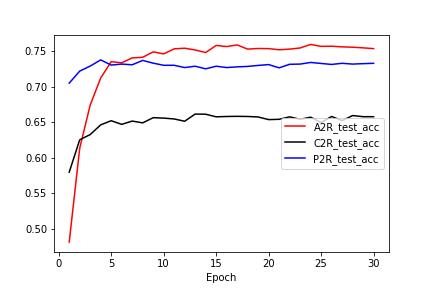
\includegraphics[scale=0.4]{HDaNN/DaNN_fig2.png}}
    \caption{DaNN: part 2}
    \label{fig:DaNN2}
\end{figure}

From figure~\ref{fig:DaNN2} we notice that $A2R$ converge more slowly than $C2R$ and $P2R$ but it can reach the highest testing accuracy. The accuracy of $P2R$ is slightly lower than $A2R$ while the testing accuracy of $C2R$ is much lower. The result is consistent with the results of most traditional methods and the situation without domain adaptation method.

Then we begin to evaluate the influence of some parameters of this model.

The third part is about parameter $\lambda$. $\lambda$ in this model means the coefficient of mmd\_loss in the calculation of total loss which theoretically can change the optimized direction. In this part we set $DR = 0.5$, $BS = 64$ and choose $A2R$ be the combination of source domain and target domain. Figure~\ref{fig:DaNN3} shows the result.
\begin{figure}[!h]
    \centerline{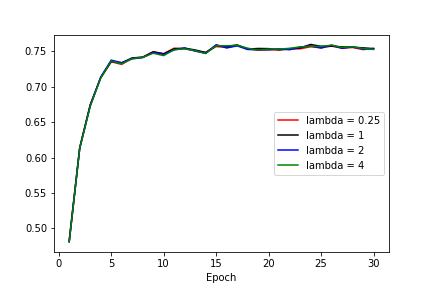
\includegraphics[scale=0.4]{HDaNN/DaNN_fig3.png}}
    \caption{DaNN: part 3}
    \label{fig:DaNN3}
\end{figure}

Something strange happens in figure~\ref{fig:DaNN3}. Almost all the curves are coincident with others, which means that parameter $\lambda$ does not play a key role in DaNN model. But there must be some other reason. We think it is because DaNN is used to deal with raw image pixels or SURF features but we change it to deal with deep learning features. This change may make $\lambda$ useless.

The fourth part is about parameter $BS$. $BS$ means the batch size of every training batch. In this part we set $DR = 0.5$, $\lambda = 1$ and choose $A2R$ be the combination of source domain and target domain. Figure~\ref{fig:DaNN4} shows the result.

\begin{figure}[!h]
    \centerline{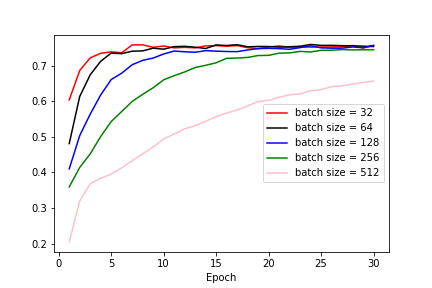
\includegraphics[scale=0.4]{HDaNN/DaNN_fig4.png}}
    \caption{DaNN: part 4}
    \label{fig:DaNN4}
\end{figure}

From figure~\ref{fig:DaNN4} we can easily find that a small batch size is better than a big batch size in this experiment. A smaller batch size can converge more quickly and when batch size is too big, its testing accuracy can not get as high as a small batch size.

The fifth part is about parameter $DR$. $DR$ means drop rate, which is used to deactivate neuron and suppress overfitting.  In this part we set $BS = 64$, $\lambda = 1$ and choose $A2R$ be the combination of source domain and target domain. Figure~\ref{fig:DaNN5} shows the result.
\begin{figure}[!h]
    \centerline{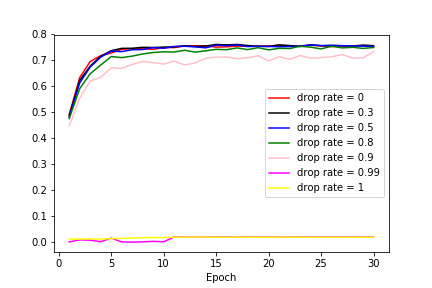
\includegraphics[scale=0.4]{HDaNN/DaNN_fig5.png}}
    \caption{DaNN: part 5}
    \label{fig:DaNN5}
\end{figure}

From figure~\ref{fig:DaNN5} we find when $DS <= 0.8$, there is almost no difference. When $DS = 0.9$, the accuracy begin to flop. And when $Ds>=0.99$, the accuracy is close to 0. It is because when drop rate is too high, most neurons are deactivated and there are not enough information to be output.
\subsubsection{ADDA Experiments}
We will present six experiments in this part. We use fully connected networks (FCNs) to construct the four subnetworks. First we show some common parameters of all of these experiments in table \ref{tab:SymADDA}. We split both $X_s$ and $X_t$ into training set, $X^{tr}_s$ and $X^{tr}_t$, and test set, $X^{te}_s$ and $X^{te}_t$. $X^{tr}_s$ is used to train ADDA the first stage and $X^{te}_s$ is used to select the best parameters of $M_s$ and $C$ correspondingly, preventing overfitting. $X^{te}_t$ is used to train ADDA the second stage and $X^{te}_t$ is used to select the best parameters of $M_t$ and $D$ correspondingly, also preventing overfitting. It should be mentioned that both $X^{te}_t$ and $X^{tr}_t$ are unlabeled. And the splitting is not always necessary since domain adaptation usually assumes all of source domain data $X_s$ as training set and all of target test data $X_t$ as test set.
 \begin{table}[h]
	\centering
	\caption{Hyper-parameters of ADDA}
	\label{tab:SymADDA}
	\begin{tabular}{ccc}
		\hline
		Symbol & Value & Description \\
		\hline
		\hline
        $K$ & $65$ & Number of classes \\
		$s$ & $5e-5$ & Optimization step \\
		$b$ & $256$ & Batch size \\
		$l_e$ & ${2048,2048}$ & Layers of $M_s$ and $M_t$ \\
		$l_c$ & ${1024,K}$ & Layers of $C$, connected from o$M_c$ or $M_t$  \\
		$l_d$ & ${512,512,2}$ & Layers of $D$, connected from $M_c$ or $M_t$ \\
        $p_k$ & $0.05$ & Dropout probability of a neuron. \\
        $l_2$ & $1e-5$ & L2 regularization for weight parameters.  \\
        $r^{tr}_{s}$ & $0.9$ & Ratio of $X_s$ used as training set.\\
        $r^{tr}_{t}$ & $0.6$ & Ratio of $X_t$ used as training set.  \\
        $I$ & $8000$ & Total iterations of first two training stages.   \\
		\hline
	\end{tabular}
\end{table}

 \begin{table*}[h]
	\centering
	\caption{Different Configurations And Resulted Performances of ADDA Experiments}
	\label{tab:ConfigADDA}
	\begin{tabular}{ccccccccccc}
		\hline
		Sym & Src & PT & AN & BN & $Ac(M_s(X^{te}_s))^*$ & $Ac(M_s(X^{te}_t))^*$ & $Ac(M_t(X^{tr}_t))^*$ & $Ac(M_t(X^{te}_t))^*$ & $g^{te}$ & $g^{tr}$\\
		\hline
		\hline
        $Ex1$ & Art & $\times$ & $\times$ & $\times$ & 0.6074 & 0.5080 & 0.0222 & 0.0189  & -0.4891 & -0.4858\\
		$Ex2$ &  Art & \checkmark & $\times$ & $\times$ & 0.6818 & 0.5712 & 0.5897 & 0.5821 & 0.0109 & 0.0185\\
		$Ex3$ &  Art & \checkmark & \checkmark & $\times$ & 0.6488 & 0.6223 & 0.6551 & 0.6372 & 0.0149& 0.0328\\
		$Ex_A$ &  Art & \checkmark & \checkmark & \checkmark & 0.7893 & 0.7313 & 0.7621 & 0.7354 & 0.0041& 0.0308\\
		$Ex_C$ &  Clipart & \checkmark & \checkmark & \checkmark & 0.8624 & 0.6561 & 0.6646 & 0.6636 & 0.0075& 0.0085\\
		$Ex_P$ &  Product & \checkmark & \checkmark & \checkmark & 0.9391 & 0.7313 & 0.7556 & 0.7353 & 0.0040& 0.0243\\
		\hline
	\end{tabular}
\end{table*}
Then we present a overview of different configurations of the six experiments and the corresponding results in table \ref{tab:ConfigADDA}. Target domain of all of the experiments presented is real world. Src is short for source data domain. PT stands for whether to transfer parameters of $M_s$ to $M_t$ for $M_t$'s initialization. AN means whether to apply learning rate annealing. BN means whether to apply batch normalization for each layer. Besides, we uses RELU function for hidden layer's activation and adds a softmax layer before calculating cross entropy. With learning rate annealing applied, we have learning rate of stage pre-training and adversarial adaptation to be $l_{r1}=\frac{1.5 \times s}{1.0 + 0.01 \times i}$ and $l_{r2}=\frac{0.1 \times s}{1.0 + 0.01 \times i}$, where $i$ it the iteration number. Otherwise, $l_{r1}=s$ and $l_{r2}=0.05 \times s$. We acquired these formulas by preliminary experiments.

$Ac(x)^*$ indicates the best accuracy towards indicator $x$. For example, in the formula $Ac(M_t(X^{te}_t))^*$, $X^{te}_t$, $M_t$ and $Ac^*$ stands for test set of unlabeled target domain, target encoder and the best accuracy respectively. Thus, $Ac(M_t(X^{te}_t))^*$ means the best test classification accuracy on target test set using target encoder. $Ac(M_t(X^{te}_t))^*$ is actually the final classification evaluation of our domain adaptation method. Similarly, $Ac(M_s(X^{te}_s))^*$ represents the best accuracy of the classifier on source test dataset using source encoder, which can be viewed as an upper bound of $Ac(M_t(X^{tr}_t))^*$. $Ac(M_t(X^{tr}_t))^*$ represents the best accuracy of the classifier on target training dataset using target encoder, which also can be viewed as an upper bound of $Ac(M_t(X^{te}_t))^*$. So, we theoretically have $Ac(M_s(X^{te}_s))^* \geq Ac(M_t(X^{tr}_t))^* \geq Ac(M_t(X^{te}_t))^*$ . As for $Ac(M_s(X^{te}_t))^*$, it represents the best accuracy of the classifier on target test dataset using source encoder. We can use $g^{te}=Ac(M_t(X^{te}_t))^*-Ac(M_s(X^{te}_t))^*$ and $g^{tr}=Ac(M_t(X^{tr}_t))^*-Ac(M_s(X^{te}_t))^*$ as the performance gain with our domain adaptation method.

Now, we go to details of the six experiments. The figures \ref{fig:Ex1}, \ref{fig:Ex2}, \ref{fig:Ex3}, \ref{fig:ExA}, \ref{fig:ExC} and \ref{fig:ExP} show visualization of the results. Four each figure, there are four subfigures showing target dataset  distribution before and after domain adaptation, classifier training history in stage pre-training, discriminator training history in stage adversarial adaptation and accuracies of $X_t$ changing in stage adversarial adaptation. Remember we combine test stage into adversarial adaptation stage. In the fourth subfigure, acc(t\_ec, training set), acc(t\_ec, test set), acc(s\_ec, training set), acc(s\_ec, test set) stands for $Ac(M_t(X^{tr}_t))$, $Ac(M_t(X^{te}_t))$, $Ac(M_s(X^{tr}_t))$ and $Ac(M_s(X^{te}_t))$ respectively. And all values of the loss curves are scaled to interval $[0.0, 1.0]$ for a better observation.

As illustrated in figure \ref{fig:Ex1}, the domain adaptation just shows no effect($Ac(M_t(X^{te}_t))^* < 0.03$). We would rather use the source encoder $M_s$ for our target dataset and achieves a test accuracy above 0.50. We tried Ex1 exactly the same as Eric Tzeng st al.'s work. Just we are using features of images instead of images themselves(Maybe we missed something in the paper). By observing transfer visualization(the first subfigure), the adapted target data just moved to another distribution and still obviously separated from the source data. By observing discriminator's training history(the third subfigure), we can see the discriminator loss falls fast and within 800 iterations, the discriminator can successfully distinguish $M_t(X_t)$ and $M_s(X_s)$ no matter how $M_t$ is trained. Thus, we believe it must be that a randomly initialized $M_t$ parameters are too chaotic for $M_t$ to optimize and deceive the discriminator.

To fix the problem, we decided to initialize $M_t$ parameters with trained $M_s$'s since we think the object features from source and target domain must have a lot in common and $M_t$ can be adjusted from $M_s$. As illustrated in figure \ref{fig:Ex2}, the result is much better. From discriminator's training history, we see GAN training curves. There exists a negative correlation between $L_D$ and $L_t$, represented by the blue and orange curve in the third subfigure respectively. In this experiment, the $Ac(M_t(X^{te}_t))^*$ overcomes $Ac(M_s(X^{te}_t))^*$ by about 0.01. The domain adaptation shows a positive effect. But, we found a problem that, in the stage of adversarial adaptation, $Ac(M_t(X^{te}_t))$, represented by the orange curve in the fourth subfigure, drops quickly at first(though increases then). And we found this is not a corner case, Eric Tzeng et al. mentioned the problem on the internet and suggested we try decreasing the learning rate.

So we have Ex3, shown in \ref{fig:Ex3}, we applied method of learning rate annealing. The process of $C$'s training in the pre-training stage(the second subfigure) improves a lot. It also help ease dropping of $Ac(M_t(X^{te}_t))$. However, still we found the training processes converge too slow in both stages. The $C$ doesn't seem to converge even after 8000 iterations.

To solve the problem, we tried method of batch normalization, as illustrated in \ref{fig:ExA}. The training of classifier $C$ converges within 800 iterations, far more quickly than before. Discriminator's training becomes more gently although $D$ grows too powerful for $M_t$ to deceive. And $Ac(M_t(X^{te}_t))^*$ grows to be 0.7354, far better than the previous three experiments. We are using the same dataset in the four experiments so far.

We show figures \ref{fig:ExC} and \ref{fig:ExP} at the bottom for completeness of our study. It seems domain adaptation does not work so well when it comes to transfer art dataset into real world dataset compared to clipart and product dataset thought the classifier works the best on the source dataset. We think it is because there exists a larger different between the two domains, real world and clipart.
\begin{figure*}[htb]

\centering
\begin{minipage}[t]{0.26\textwidth}
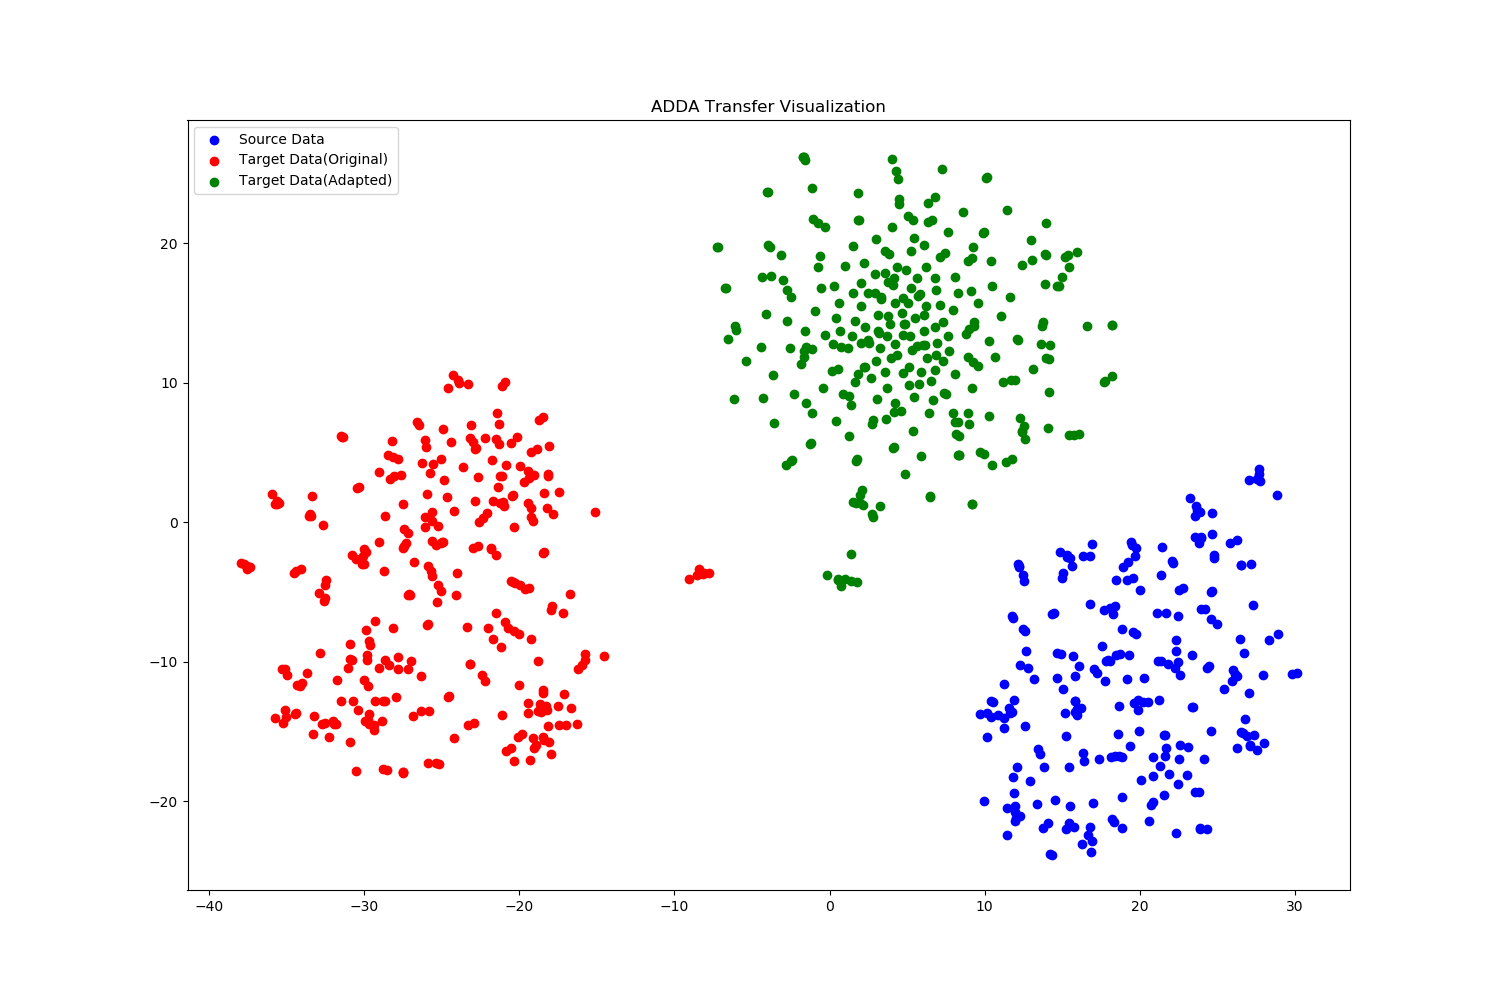
\includegraphics[width=1.6in, height=1.5in]{Ladda/A2R_no_preassign_no_dec_no_bn/ADDA_visual.png}
\end{minipage}%
\begin{minipage}[t]{0.26\textwidth}
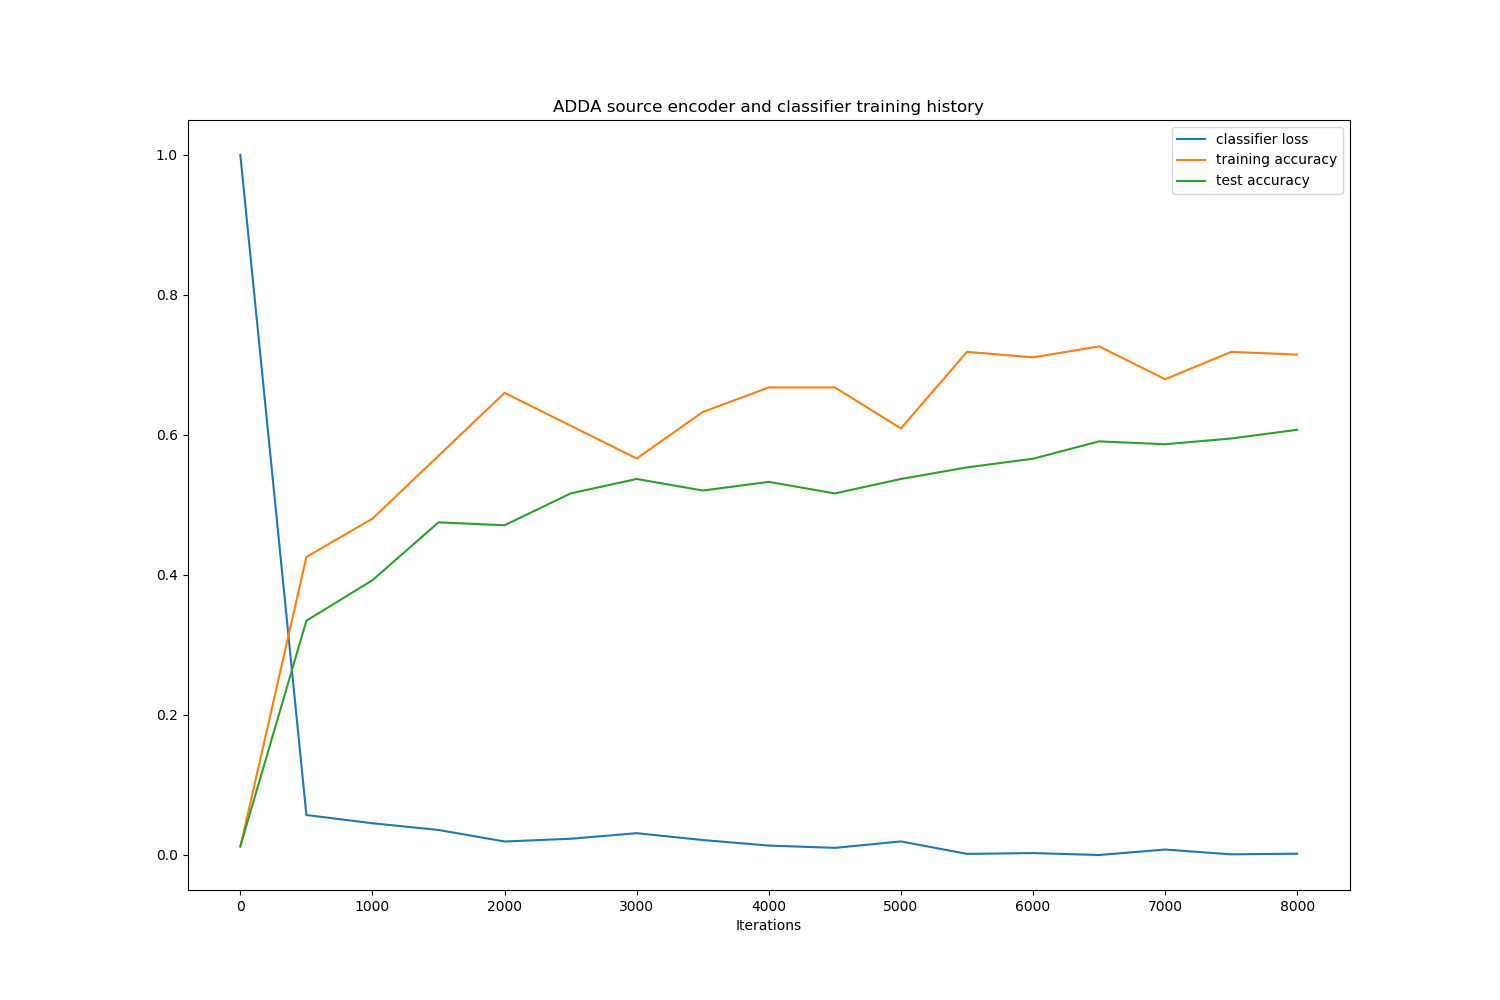
\includegraphics[width=1.6in, height=1.5in]{Ladda/A2R_no_preassign_no_dec_no_bn/clf.png}
\end{minipage}%
\begin{minipage}[t]{0.45\textwidth}
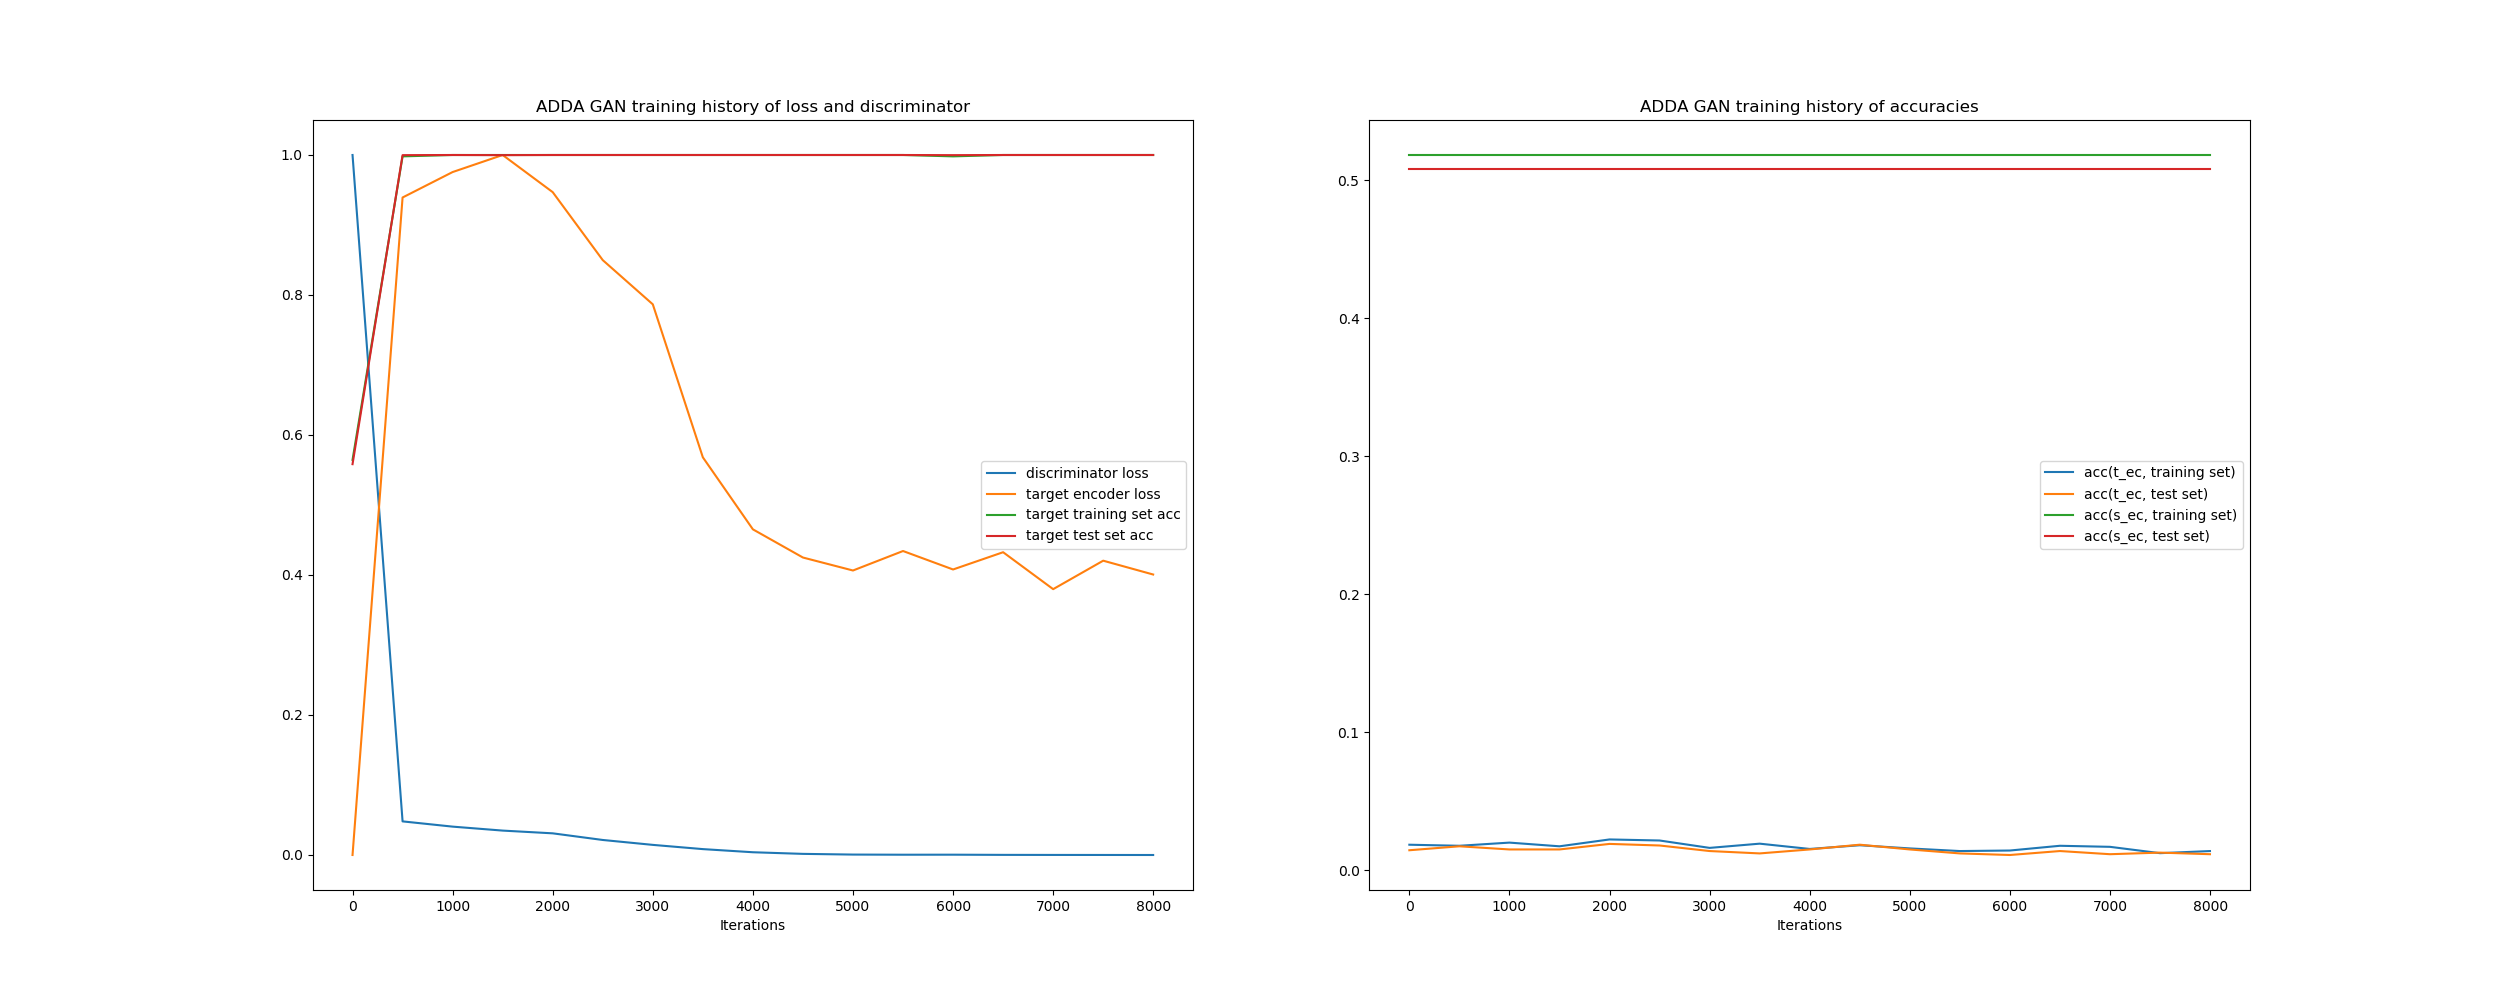
\includegraphics[width=3.5in, height=1.5in]{Ladda/A2R_no_preassign_no_dec_no_bn/gan.png}
\end{minipage}%
\caption{Visualization of ADDA Ex1 Result}\label{fig:Ex1}
\end{figure*}

\begin{figure*}[htb]

\centering
\begin{minipage}[t]{0.26\textwidth}
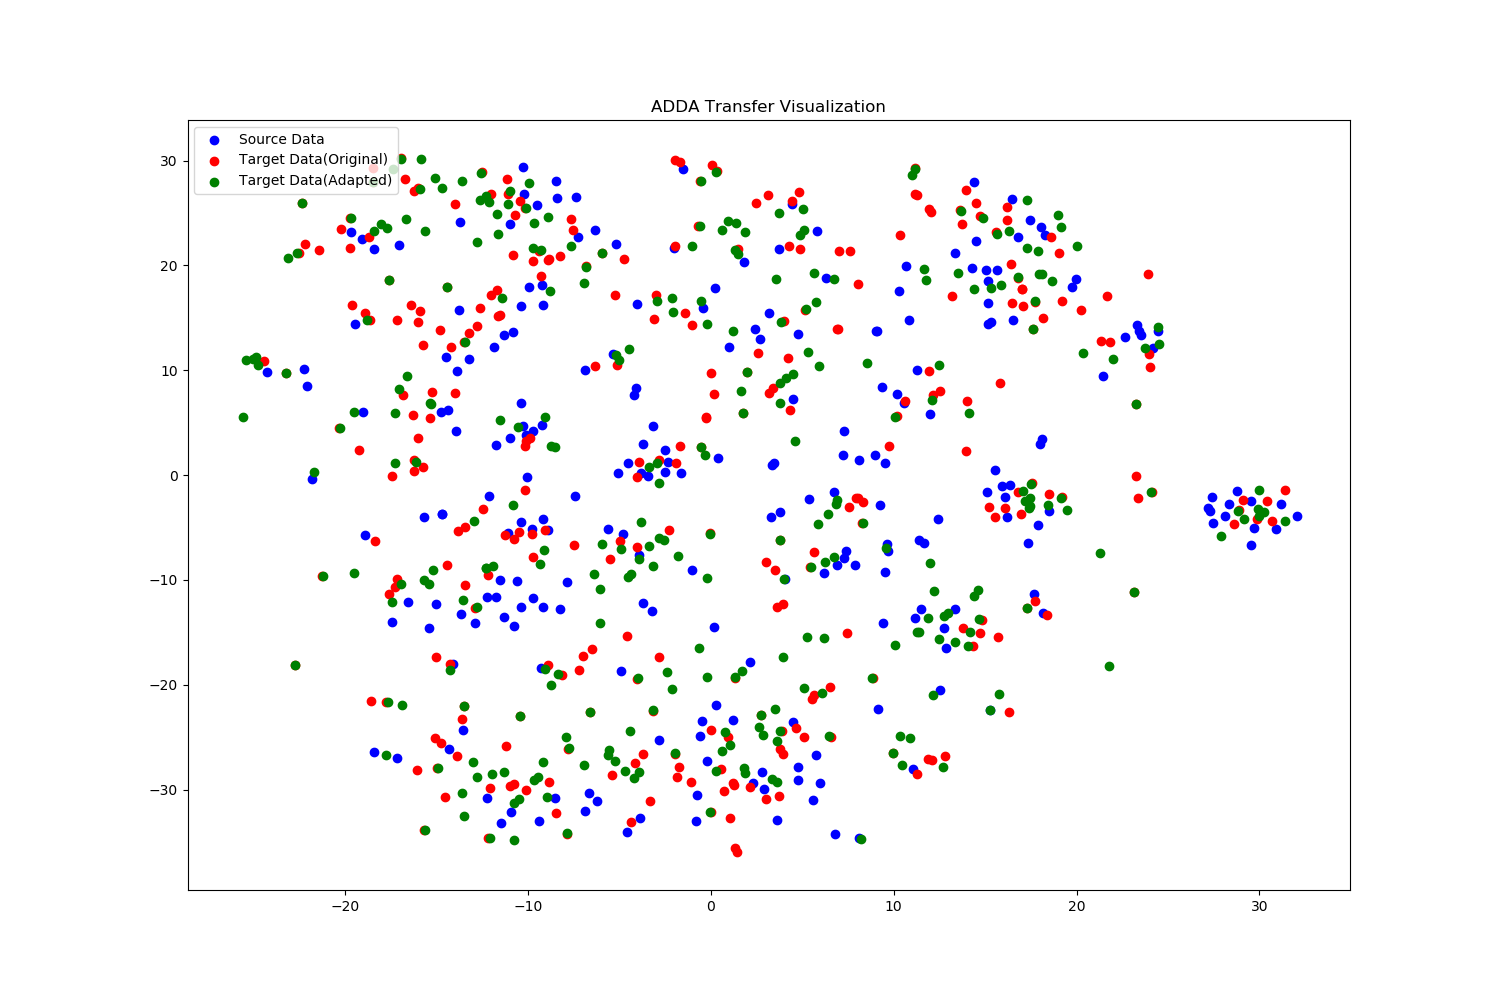
\includegraphics[width=1.6in, height=1.5in]{Ladda/A2R_no_dec_no_bn/ADDA_visual.png}
\end{minipage}%
\begin{minipage}[t]{0.26\textwidth}
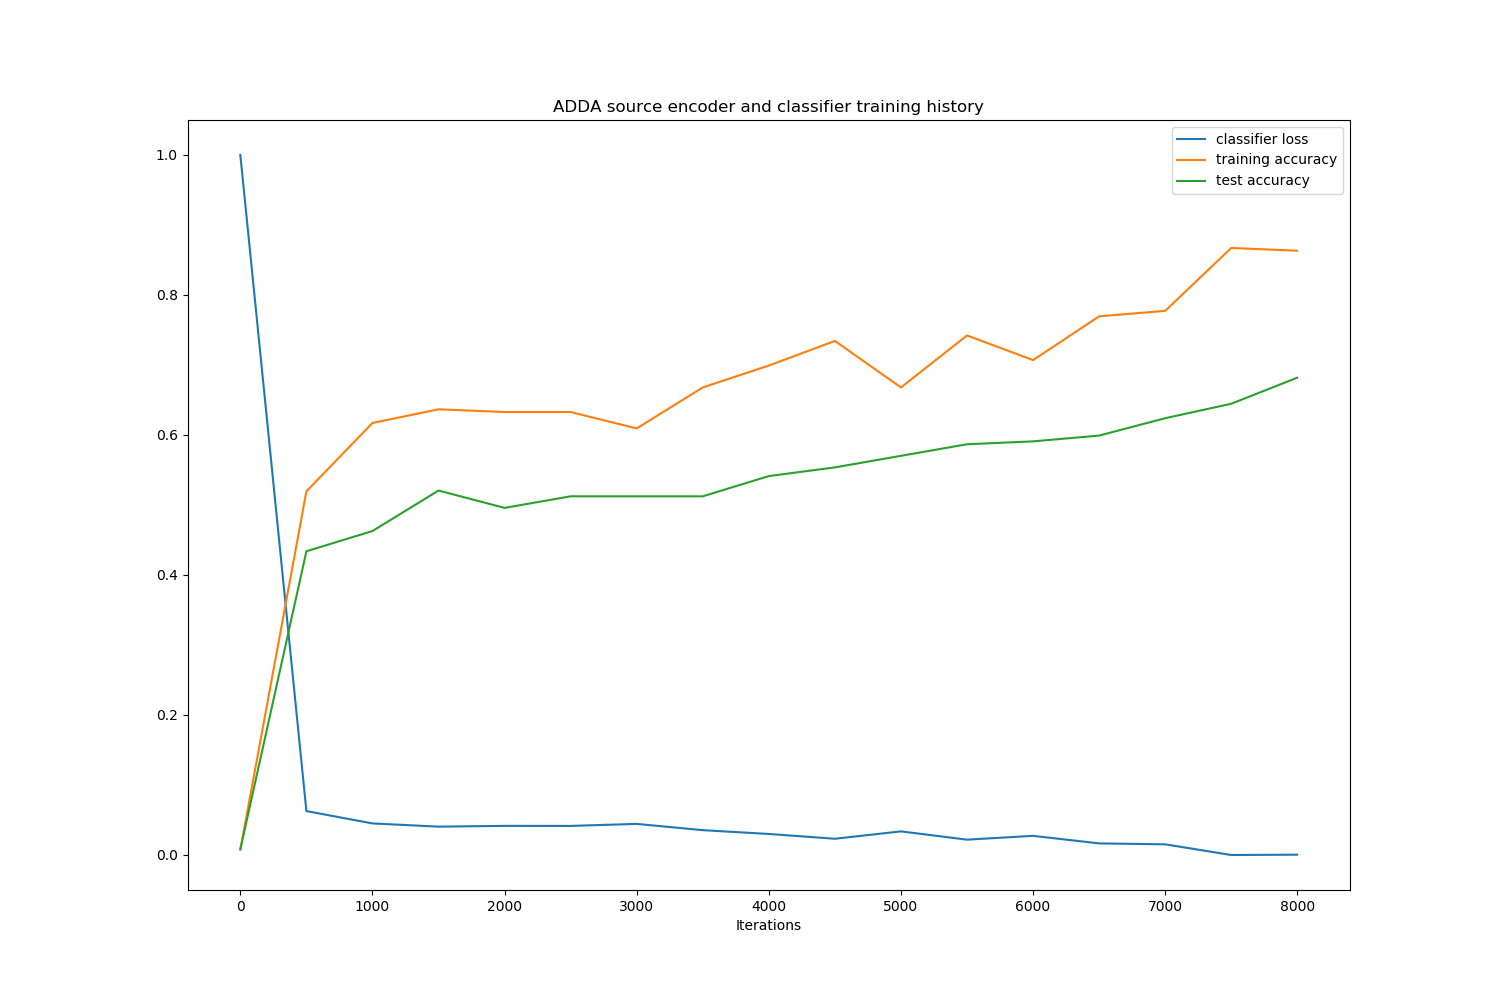
\includegraphics[width=1.6in, height=1.5in]{Ladda/A2R_no_dec_no_bn/clf.png}
\end{minipage}%
\begin{minipage}[t]{0.45\textwidth}
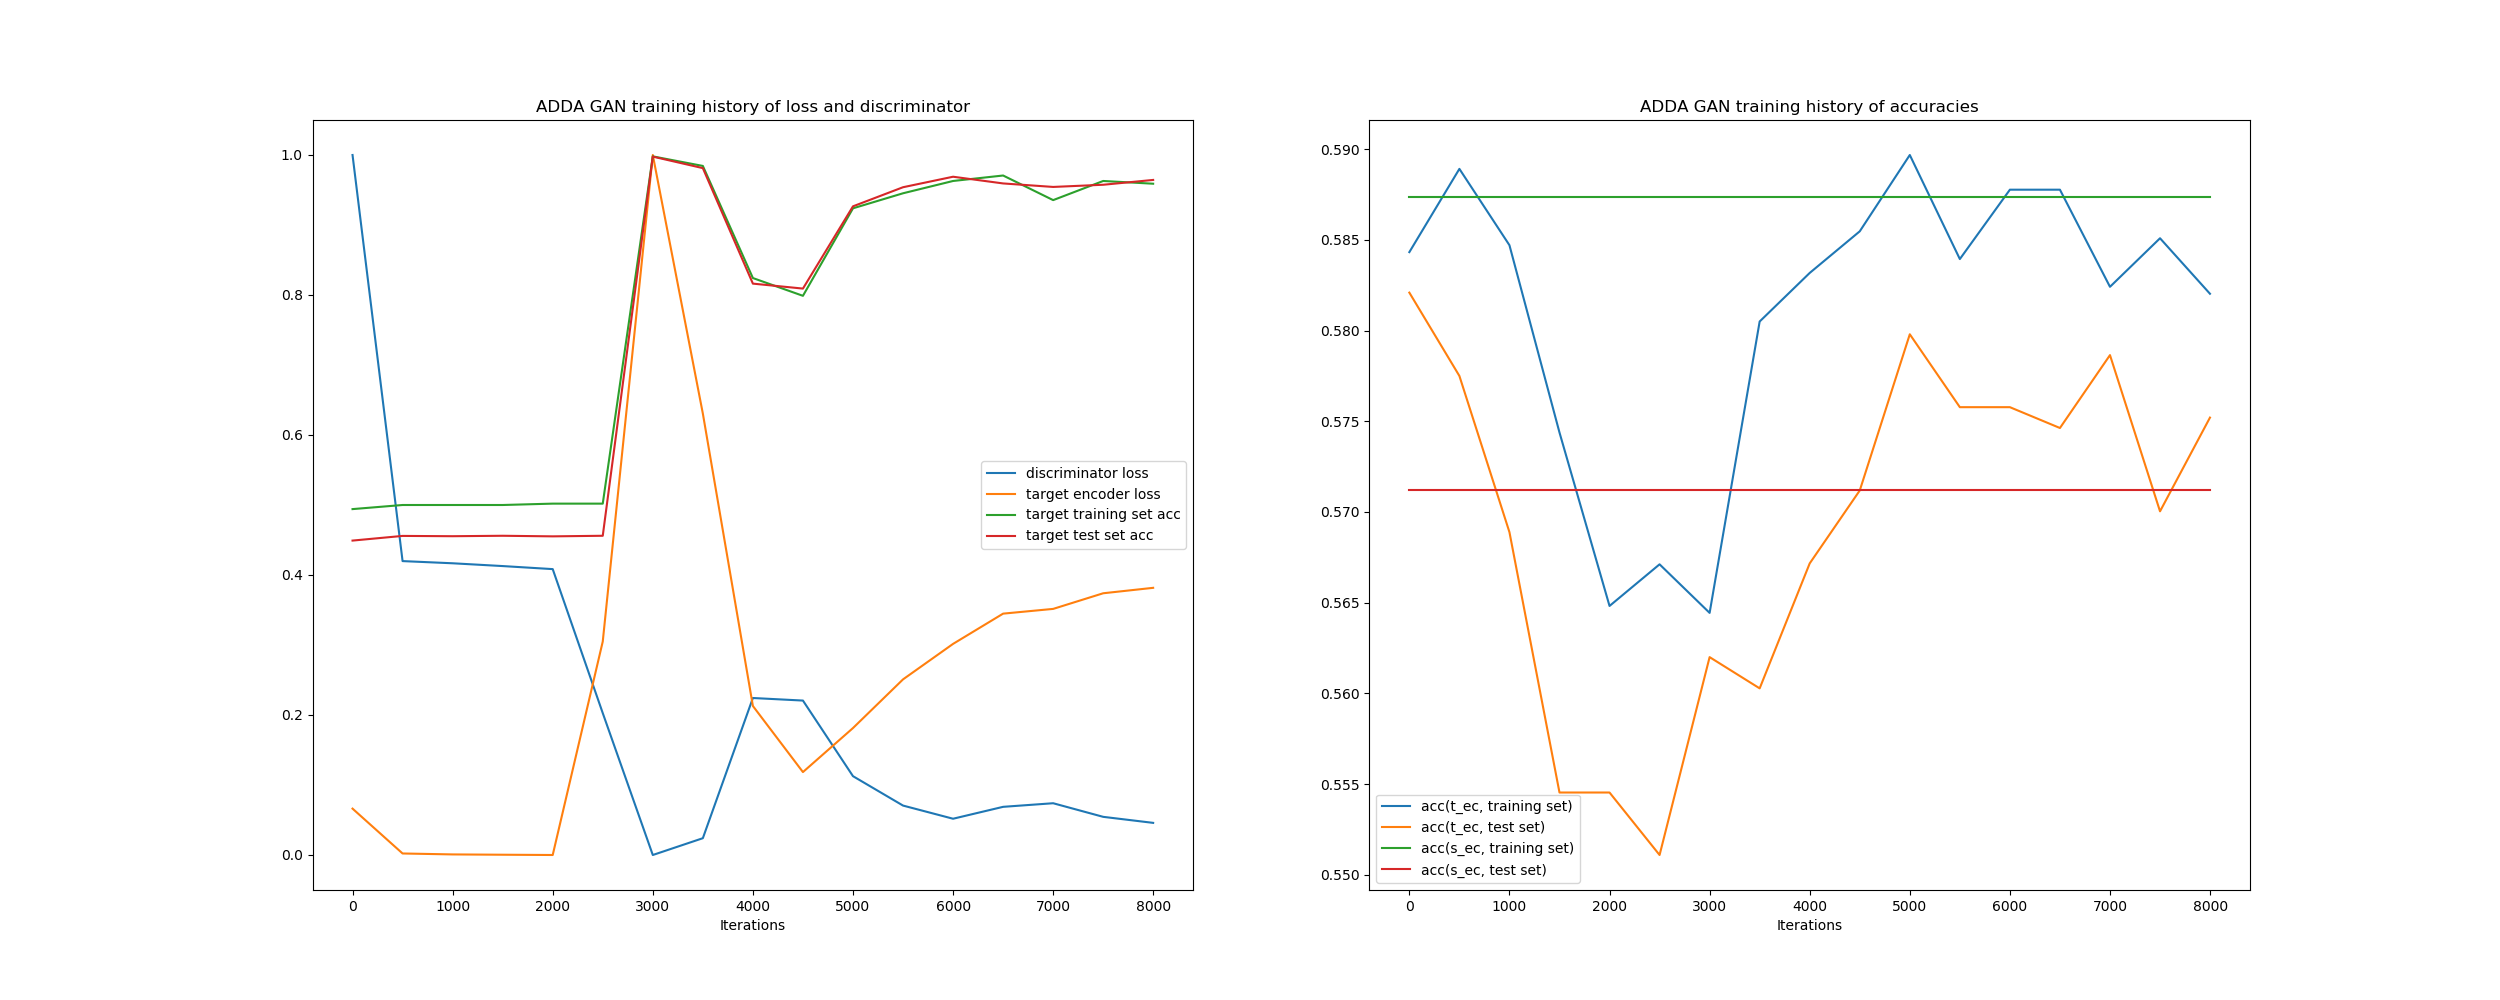
\includegraphics[width=3.5in, height=1.5in]{Ladda/A2R_no_dec_no_bn/gan.png}
\end{minipage}%
\caption{Visualization of ADDA Ex2 Result}\label{fig:Ex2}
\end{figure*}

\begin{figure*}[htb]

\centering
\begin{minipage}[t]{0.26\textwidth}
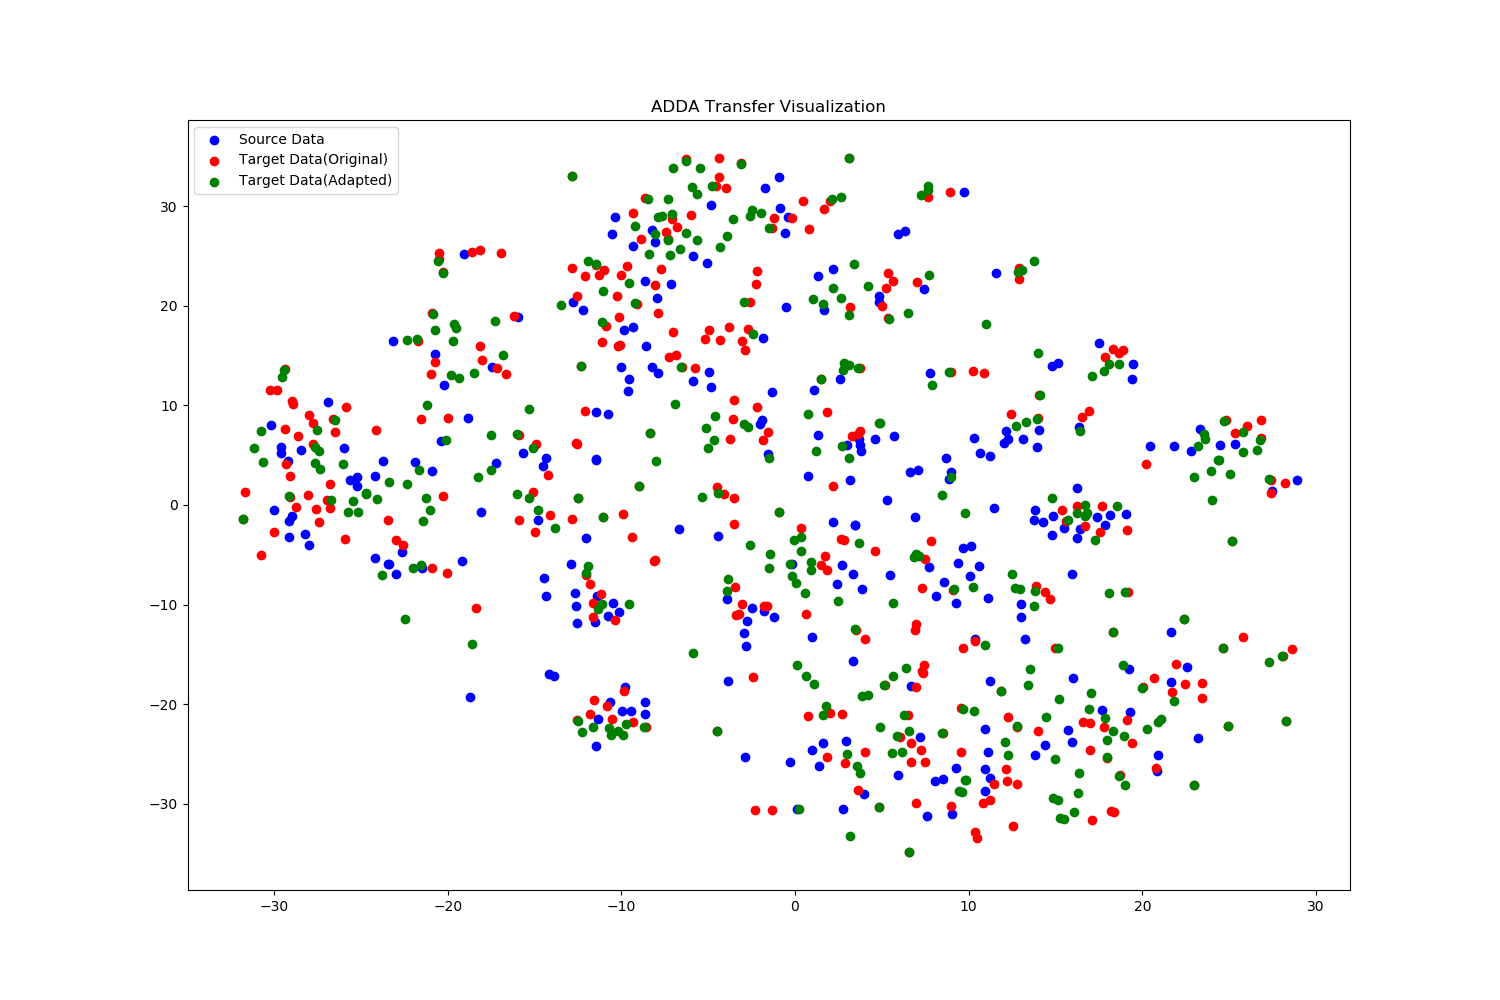
\includegraphics[width=1.6in, height=1.5in]{Ladda/A2R_no_bn/ADDA_visual.png}
\end{minipage}%
\begin{minipage}[t]{0.26\textwidth}
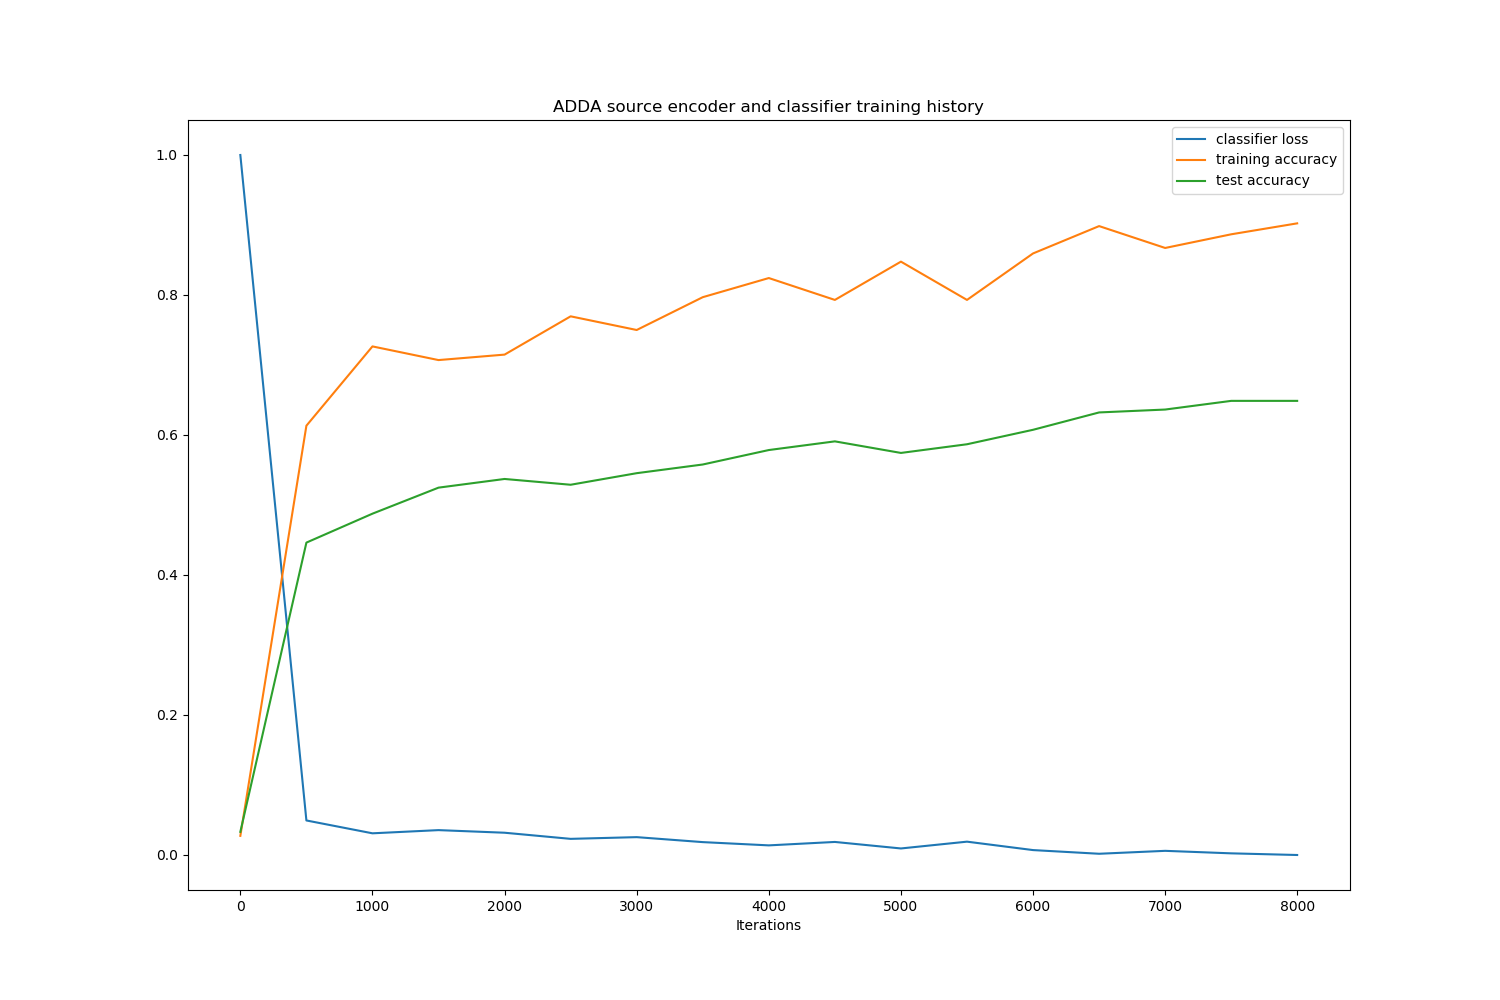
\includegraphics[width=1.6in, height=1.5in]{Ladda/A2R_no_bn/clf.png}
\end{minipage}%
\begin{minipage}[t]{0.45\textwidth}
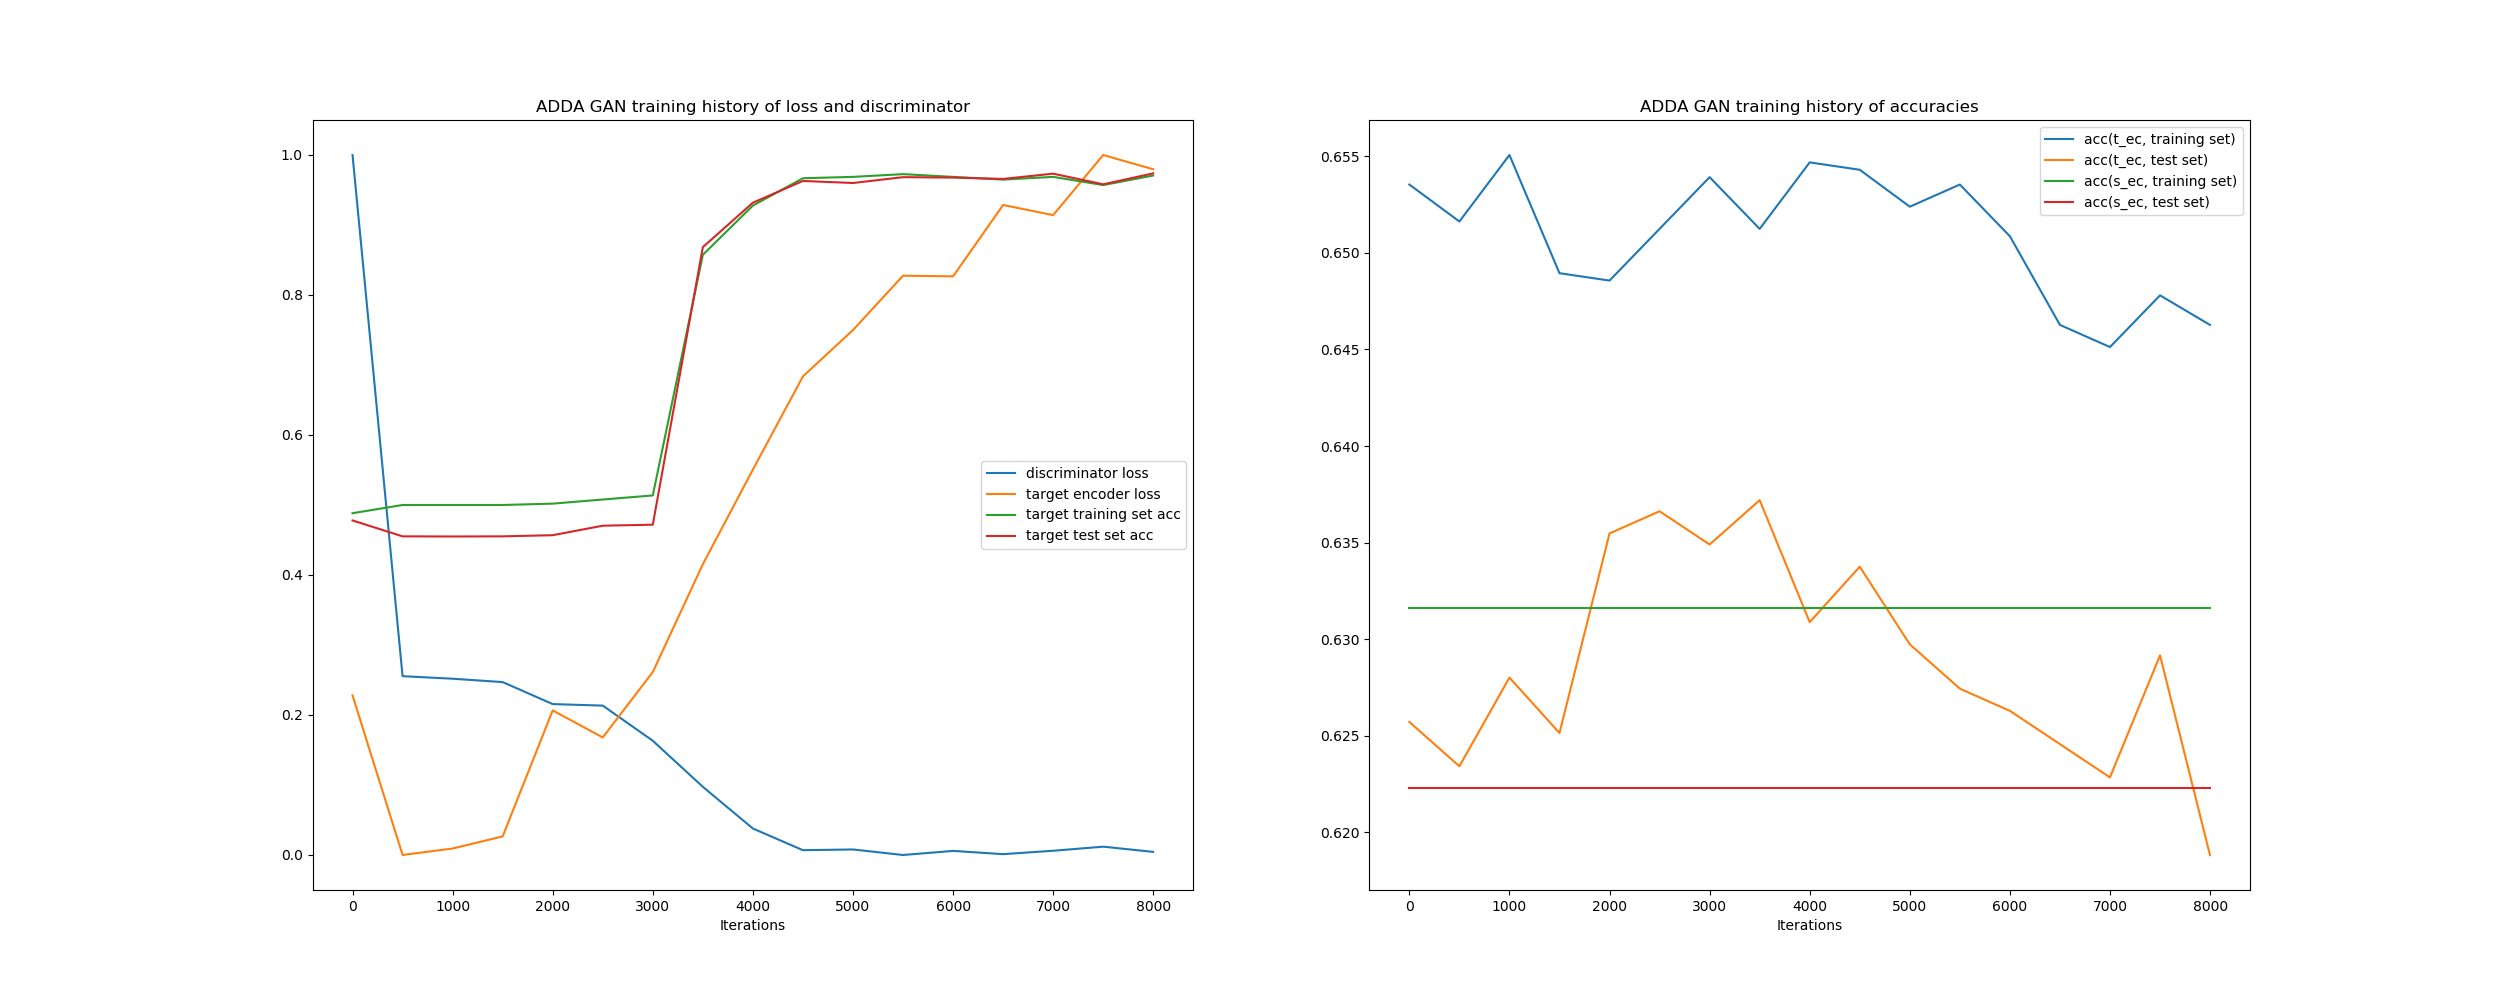
\includegraphics[width=3.5in, height=1.5in]{Ladda/A2R_no_bn/gan.png}
\end{minipage}%
\caption{Visualization of ADDA Ex3 Result}\label{fig:Ex3}
\end{figure*}

\begin{figure*}[htb]

\centering
\begin{minipage}[t]{0.26\textwidth}
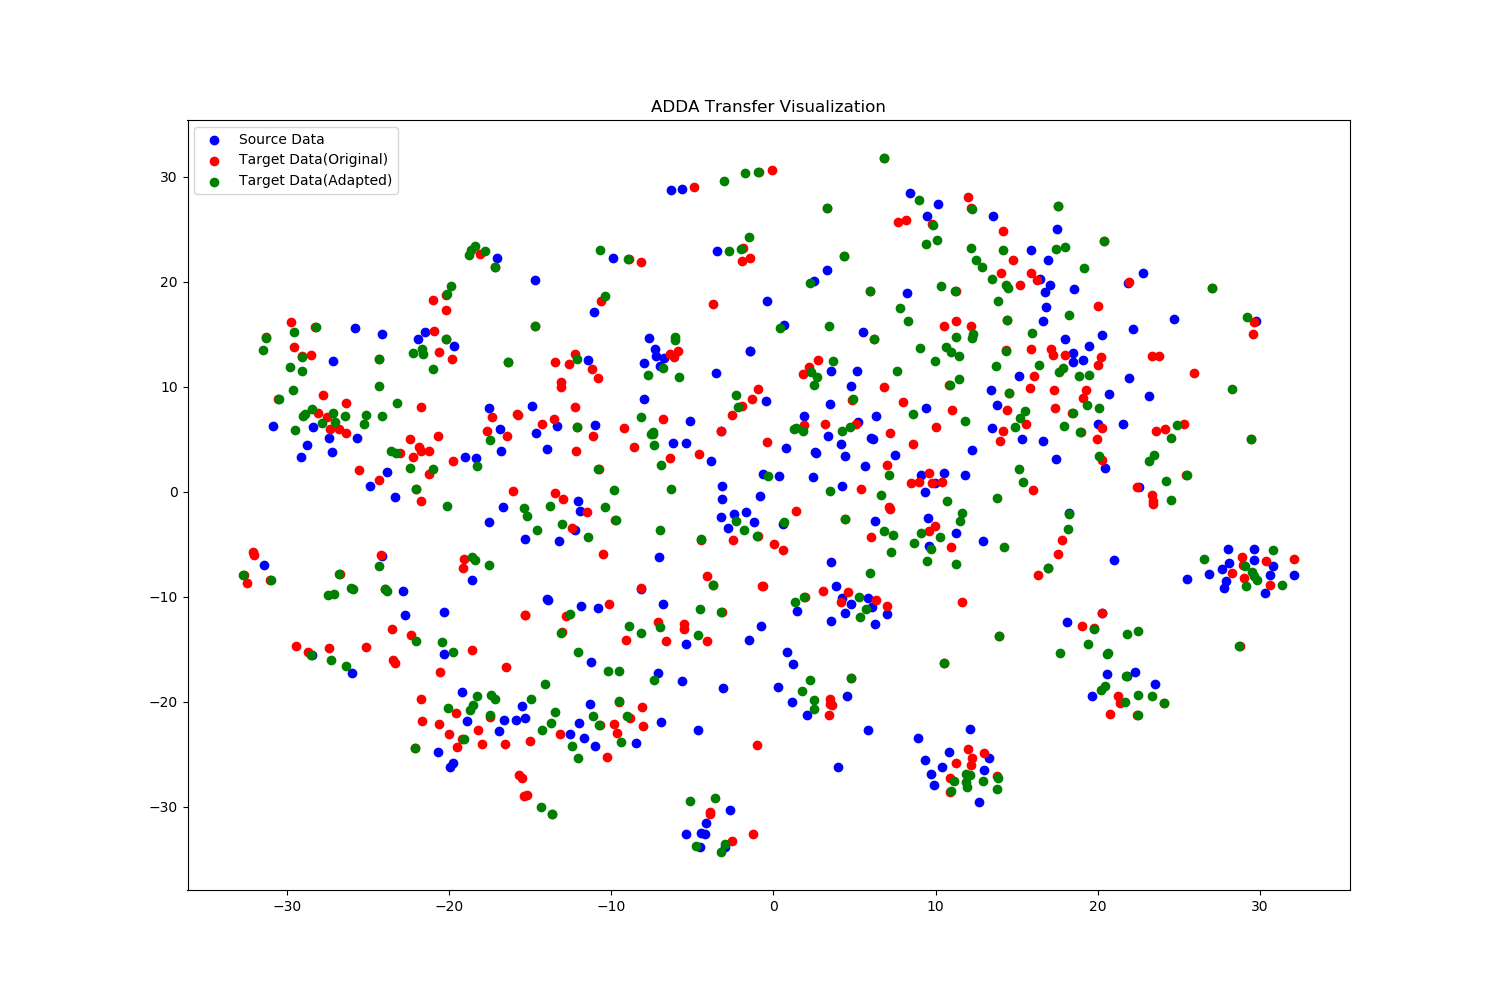
\includegraphics[width=1.6in, height=1.5in]{Ladda/std_A2R/ADDA_visual.png}
\end{minipage}%
\begin{minipage}[t]{0.26\textwidth}
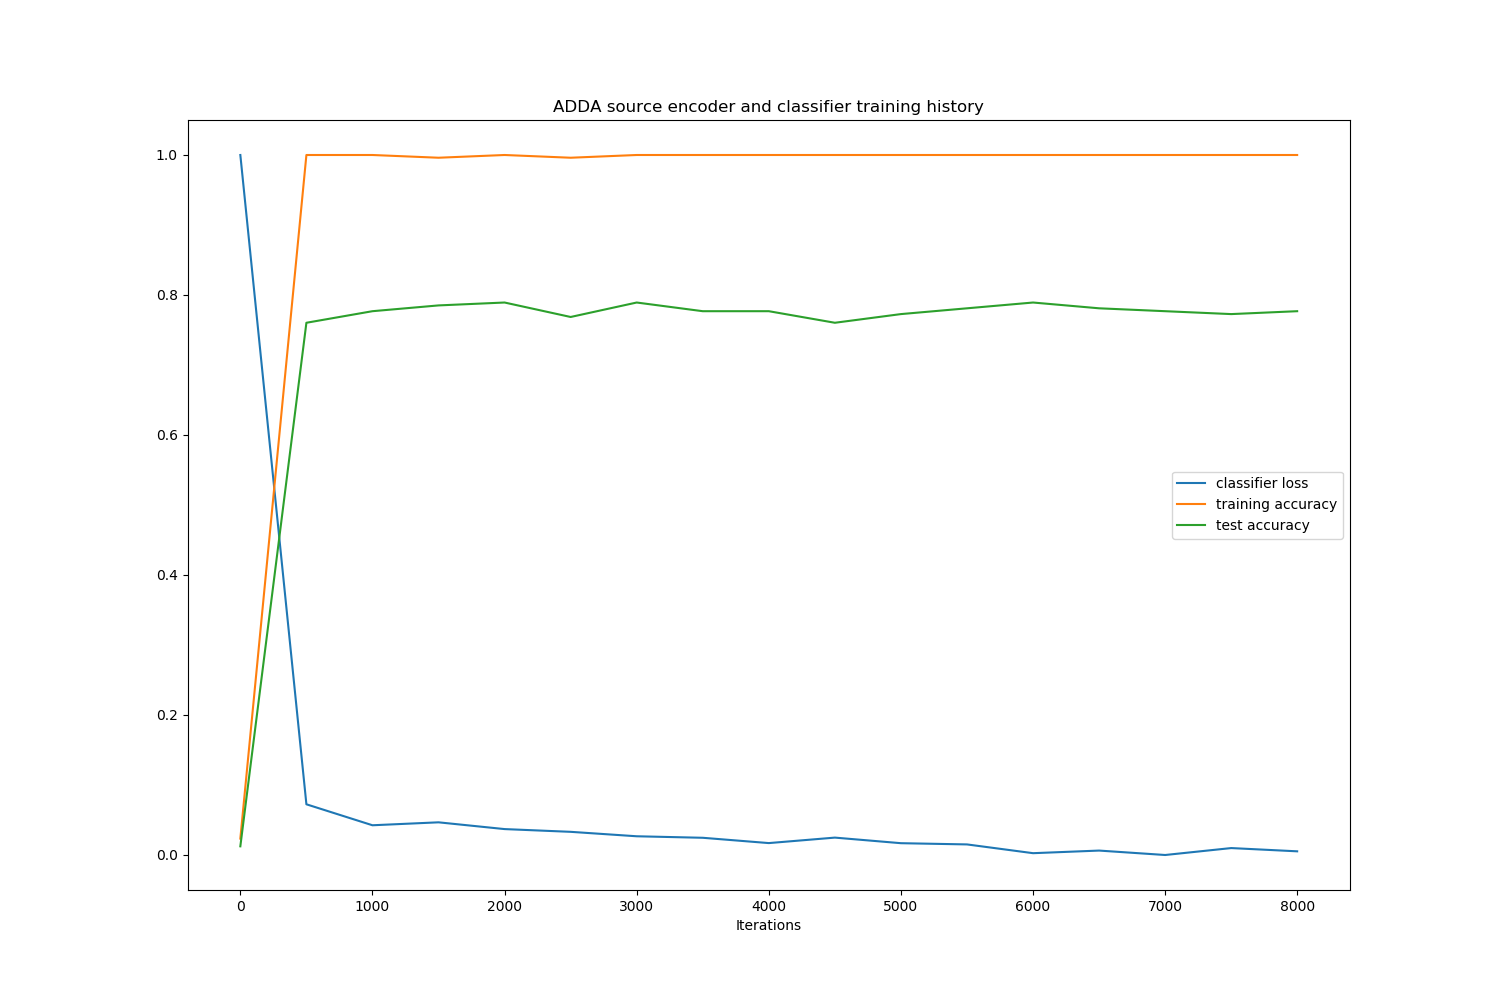
\includegraphics[width=1.6in, height=1.5in]{Ladda/std_A2R/clf.png}
\end{minipage}%
\begin{minipage}[t]{0.45\textwidth}
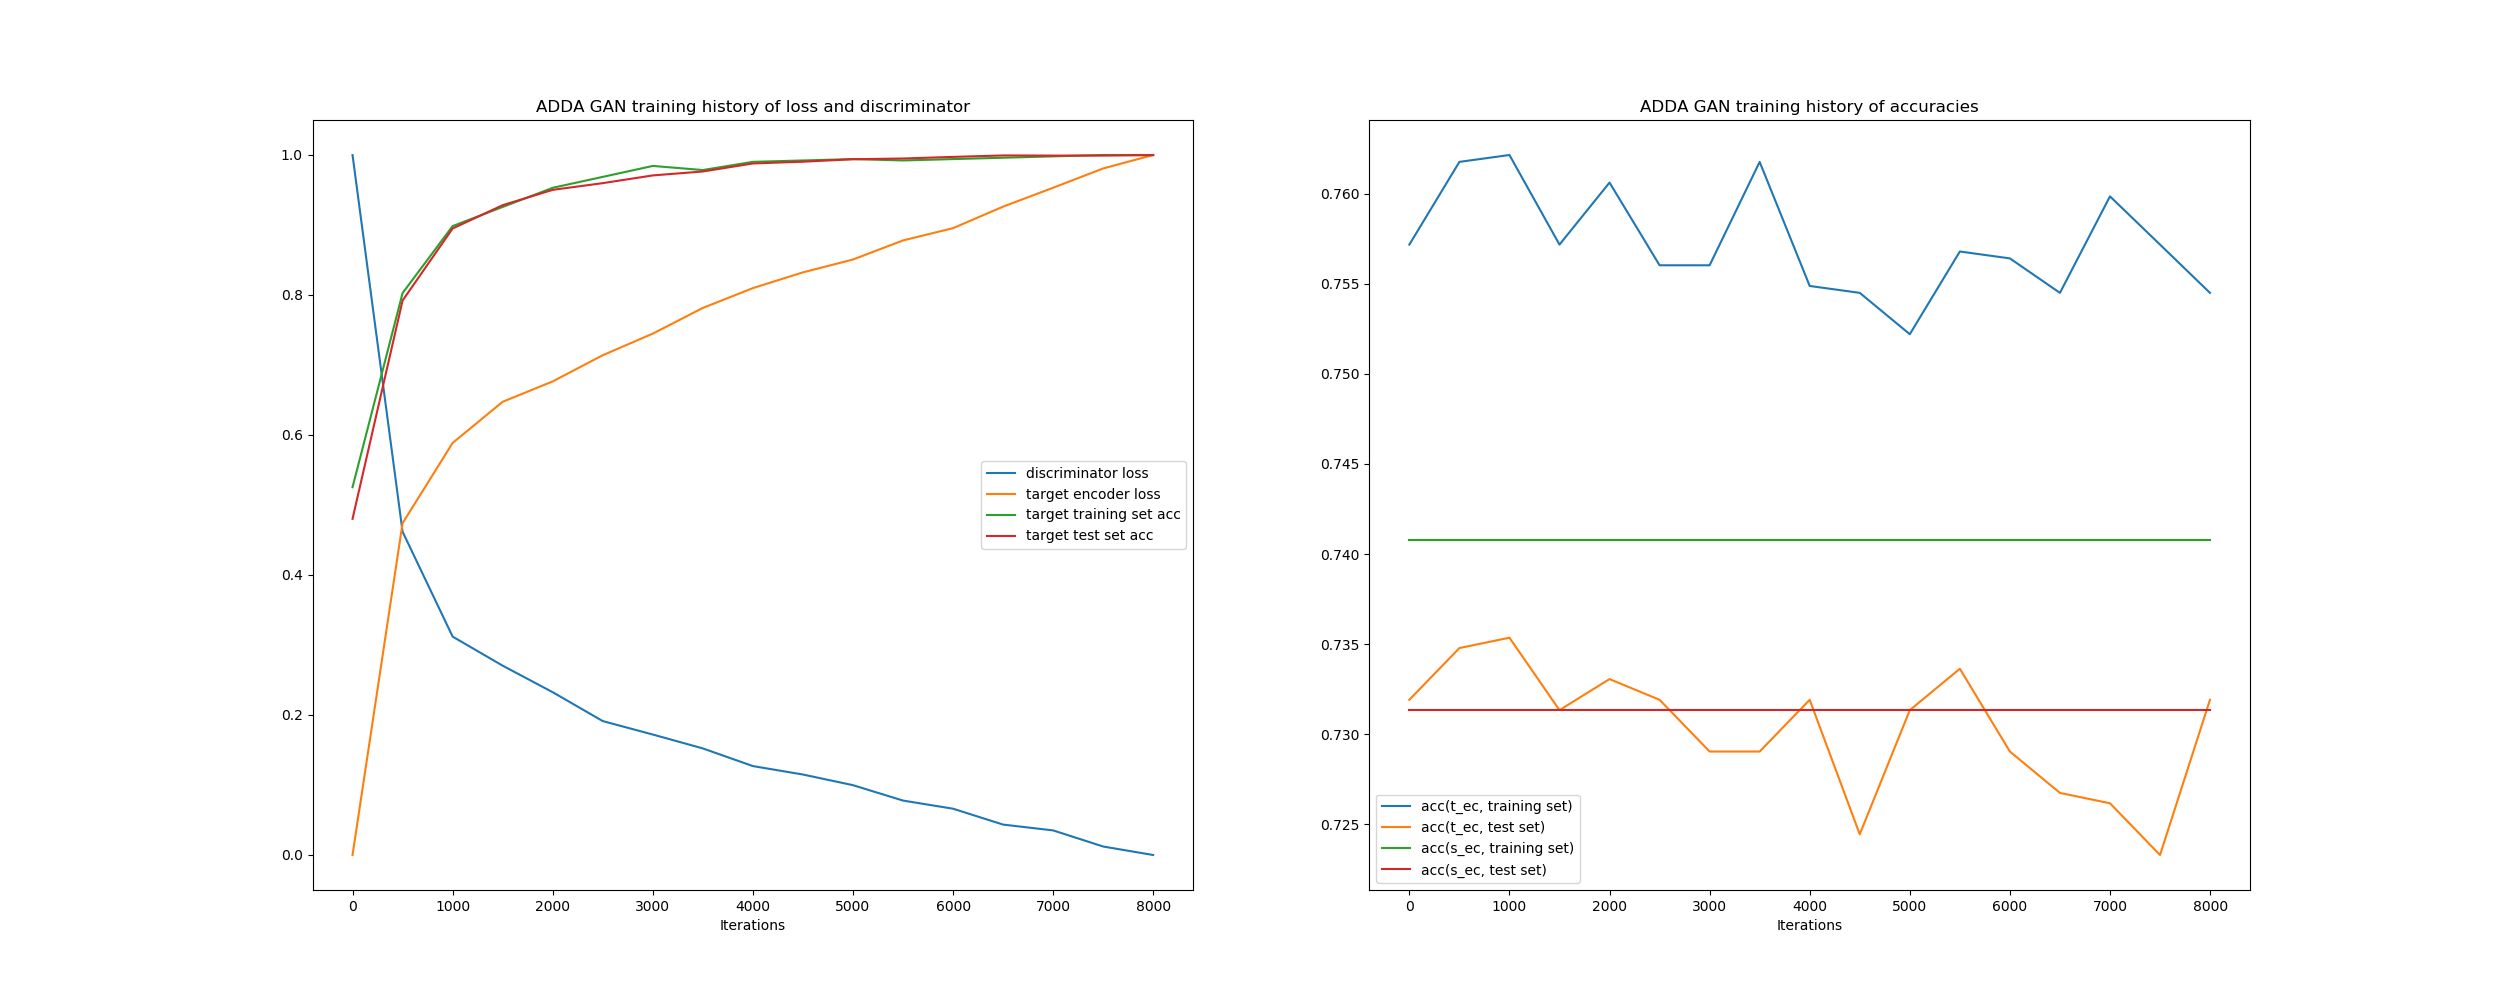
\includegraphics[width=3.5in, height=1.5in]{Ladda/std_A2R/gan.png}
\end{minipage}%
\caption{Visualization of ADDA ExA Result}\label{fig:ExA}
\end{figure*}




\subsubsection{DANN Experiments}
We present three experiments using DANN method. Because of time issue, we did not design DANN experiments that sophisticatedly, but we learned a lot from ADDA experiments. Common hyper-parameters are listed in table \ref{tab:SymDANN}. Tricks of L2 normalization and neuron dropout are not used in the experiments because these tricks did not perform that well as expected in the previous experiments of DANN. And we use sigmoid function for activation of hidden layers. Also, a softmax layer is added after the output layer before calculating cross entropy. Batch normalization is not applied in DANN experiments. DANN networks we designed are much simpler and more light-weighted. Learning rate, $l_r$, of both two stages anneals according to the formula: $l_r= \frac{0.00004}{ (1.0 + \frac{1.0 \times i}{I})^{0.75}}$, where $i$ is the current iteration. Primitive of the formula was proposed in Yaroslav Ganin, et al.'s work. We just adjust some factors according to our preliminary experiments.
 \begin{table}[h]
	\centering
	\caption{Hyper-parameters of DANN}
	\label{tab:SymDANN}
	\begin{tabular}{ccc}
		\hline
		Symbol & Value & Description \\
		\hline
		\hline
        $K$ & $65$ & Number of classes \\
		$b$ & $256$ & Batch size \\
		$l_e$ & ${2048,1024}$ & Layers of $M$ \\
		$l_c$ & ${256,K}$ & Layers of $C$, connected from o$M$  \\
		$l_d$ & ${512,512,2}$ & Layers of $D$, connected from $M$ \\
        $p_k$ & $0.0$ & Dropout probability of a neuron. \\
        $r^{tr}_{s}$ & $0.75$ & Ratio of $X_s$ used as training set.\\
        $r^{tr}_{t}$ & $0.75$ & Ratio of $X_t$ used as training set.  \\
        $I$ & $8000$ & Total iterations of first two training stages.   \\
		\hline
	\end{tabular}
\end{table}


 \begin{table*}[h]
	\centering
	\caption{Different Configurations And Resulted Performances of DANN Experiments}
	\label{tab:ConfigDANN}
	\begin{tabular}{cccccccc}
		\hline
		Sym & Src & $Ac(M_s(X^{te}_s))^*$ & $Ac(M_s(X^{te}_t))^*$ & $Ac(M_t(X^{tr}_t))^*$ & $Ac(M_t(X^{te}_t))^*$ & $g^{te}$ & $g^{tr}$\\
		\hline
		\hline
		$Ex_A$ &  Art & 0.8020 & 0.7172 & 0.7488 & 0.7301 & 0.0129 & 0.0316\\
		$Ex_C$ &  Clipart & 0.8671 & 0.6501 & 0.6683 & 0.6547 & 0.0046 & 0.0182\\
		$Ex_P$ &  Product &  0.9596 & 0.7328 & 0.7411 & 0.7392 & 0.0064 & 0.0083\\
		\hline
	\end{tabular}
\end{table*}
We first present an overview of all of the three DANN experiments in table \ref{tab:ConfigDANN}. Different from ADDA model, we have only one encoder $M$ in DANN. $M$ is trained with $(X_s, Y_x)$ in the first stage and then trained to adapt target domain in the second stage. Thus, to maintain consistency of our symbols, we use $M_s$ to represent the encoder after the first-stage training and $M_t$ to represent the encoder after the second-stage training.

Compared with the results of ADDA shown in the last three rows of table \ref{tab:ConfigADDA}, except the first-stage trained classification accuracies on source test set, $Ac(M_s(X^{te}_s))^*$, show better performances, the other three indicators fall. The classifier works better with source domain dataset after pre-training but doesn't show such improvement when it comes to classify adapted target domain data.

Figures \ref{fig:ExA2}, \ref{fig:ExC2}, \ref{fig:ExP2} shows visualization of the three DANN experiments(see the bottom for \ref{fig:ExC2} and \ref{fig:ExP2}). The are four subfigures in each figure. The first two subfigures illustrate visualization of encoded source and target data distribution before($M_s(X^{te}_s)$, $M_s(X^{te}_t)$) and after($M_t(X^{te}_s)$, $M_t(X^{te}_t)$) domain adaptation. The third subfigure shows training history of the classifier $C$ in the pre-train stage. We name feature encoder in this stage $M_s$. Legends of "source accuracy(test)" and "source accuracy(train)" represent $Ac(M_s(X^{te}_s))$ and $Ac(M_s(X^{tr}_s))$ respectively. The fourth figure shows training history of the adversarial adaptation stage. Recall that discriminator $D$ and feature encoder $M$ are trained in this stage, and we name feature encoder in this stage $M_t$.  Legends of "source accuracy(test)", "target accuracy(test)", "source accuracy(train)" and "target accuracy(train)" represent $Ac(M_t(X^{te}_s))$, $Ac(M_t(X^{te}_t))$, $Ac(M_t(X^{tr}_s))$ and $Ac(M_t(X^{tr}_t))$ respectively.

Unlike ADDA, the ability of $D$ doesn't improve so smoothly and the final discrimination accuracy, represented by red line of the fourth subfigure, maintains about $0.5$, which theoretically indicates the training of the encoder $M$ is effective. We think it is because we are not minimizing $L_C$ and $L_D$ respectively but minimizing $L_{da} = L_C+L_D$. We want to keep a good performance of classifier $C$ the same time when trying to adjust $M$ to adapt the target domain data.

\begin{figure*}[htb]
\centering
\begin{minipage}[t]{0.26\textwidth}
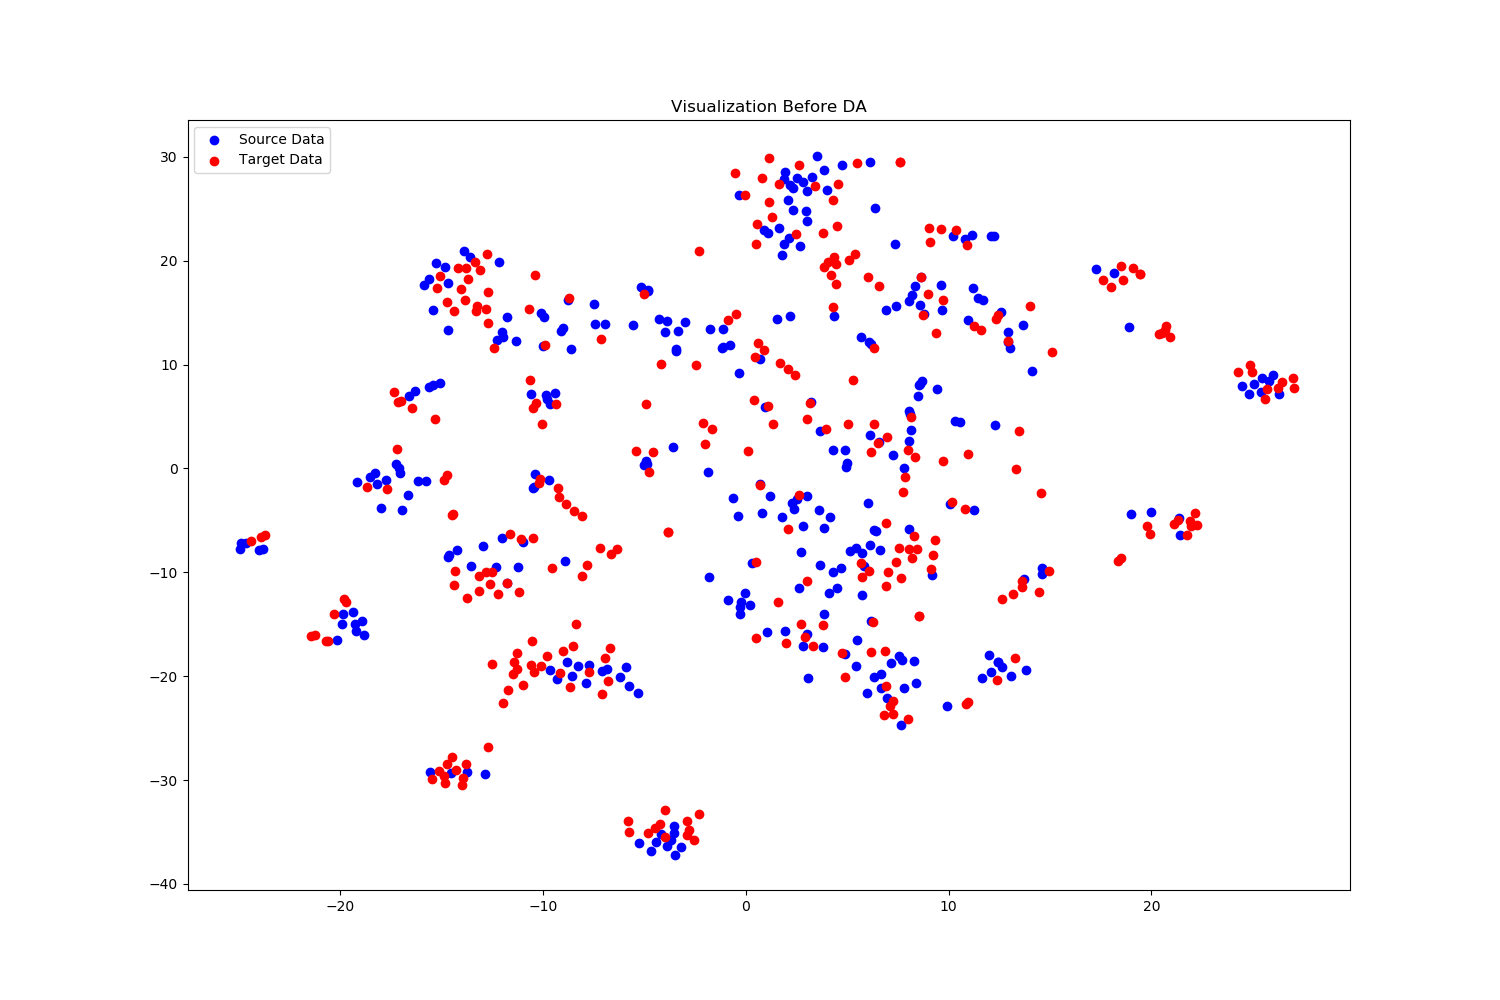
\includegraphics[width=1.6in, height=1.5in]{Ldann/std_A2R/before.png}
\end{minipage}%
\begin{minipage}[t]{0.26\textwidth}
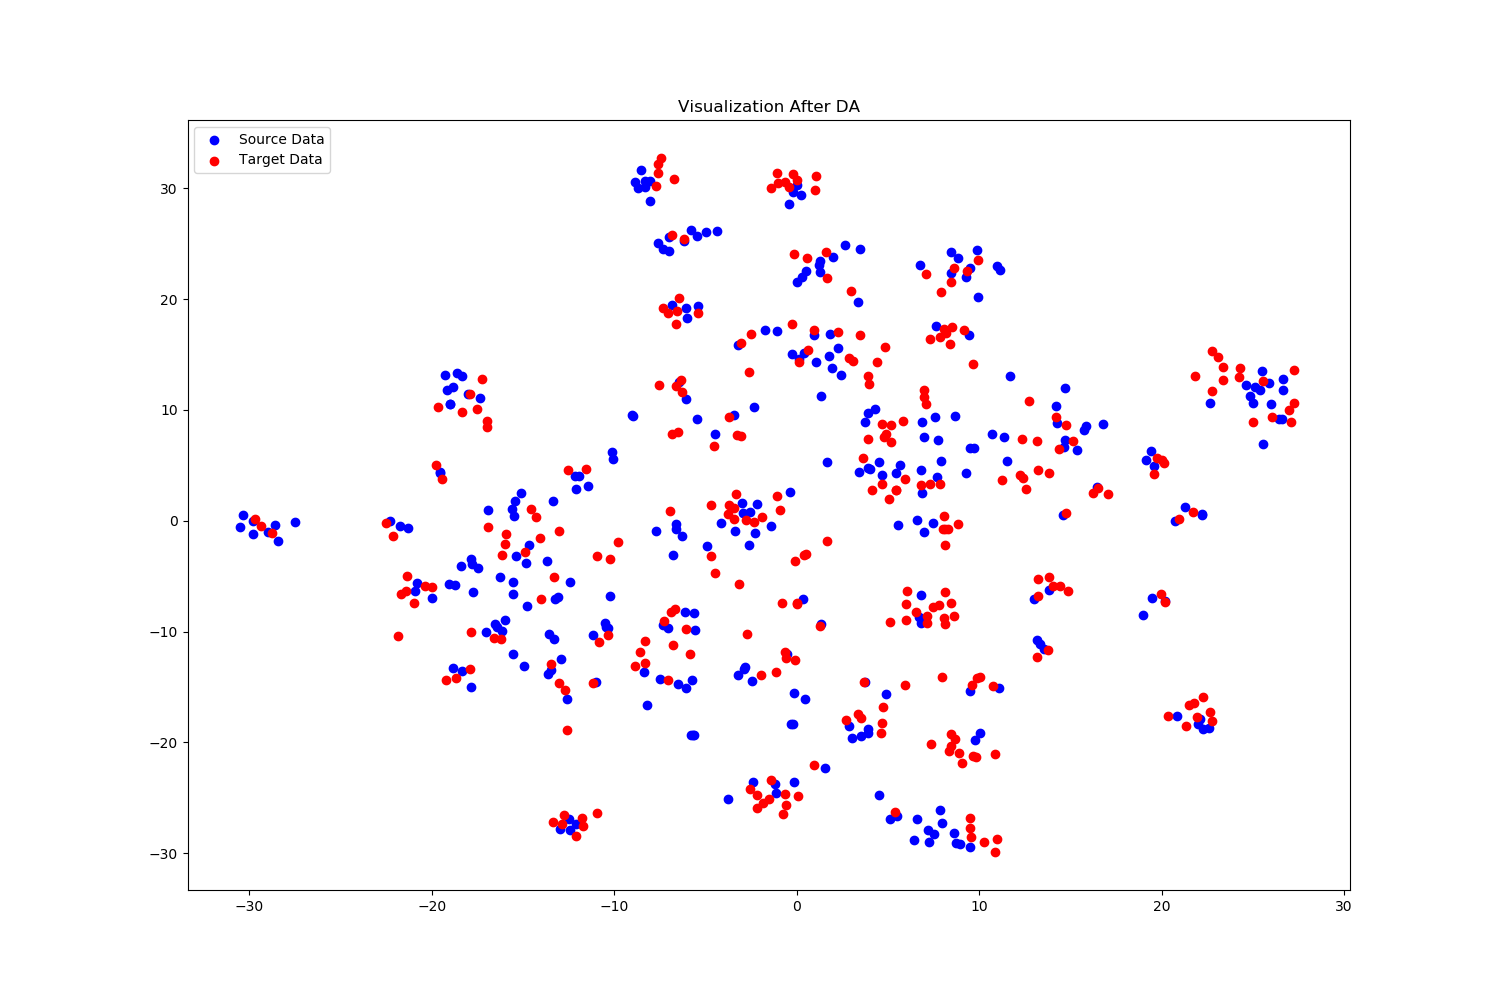
\includegraphics[width=1.6in, height=1.5in]{Ldann/std_A2R/after.png}
\end{minipage}%
\begin{minipage}[t]{0.45\textwidth}
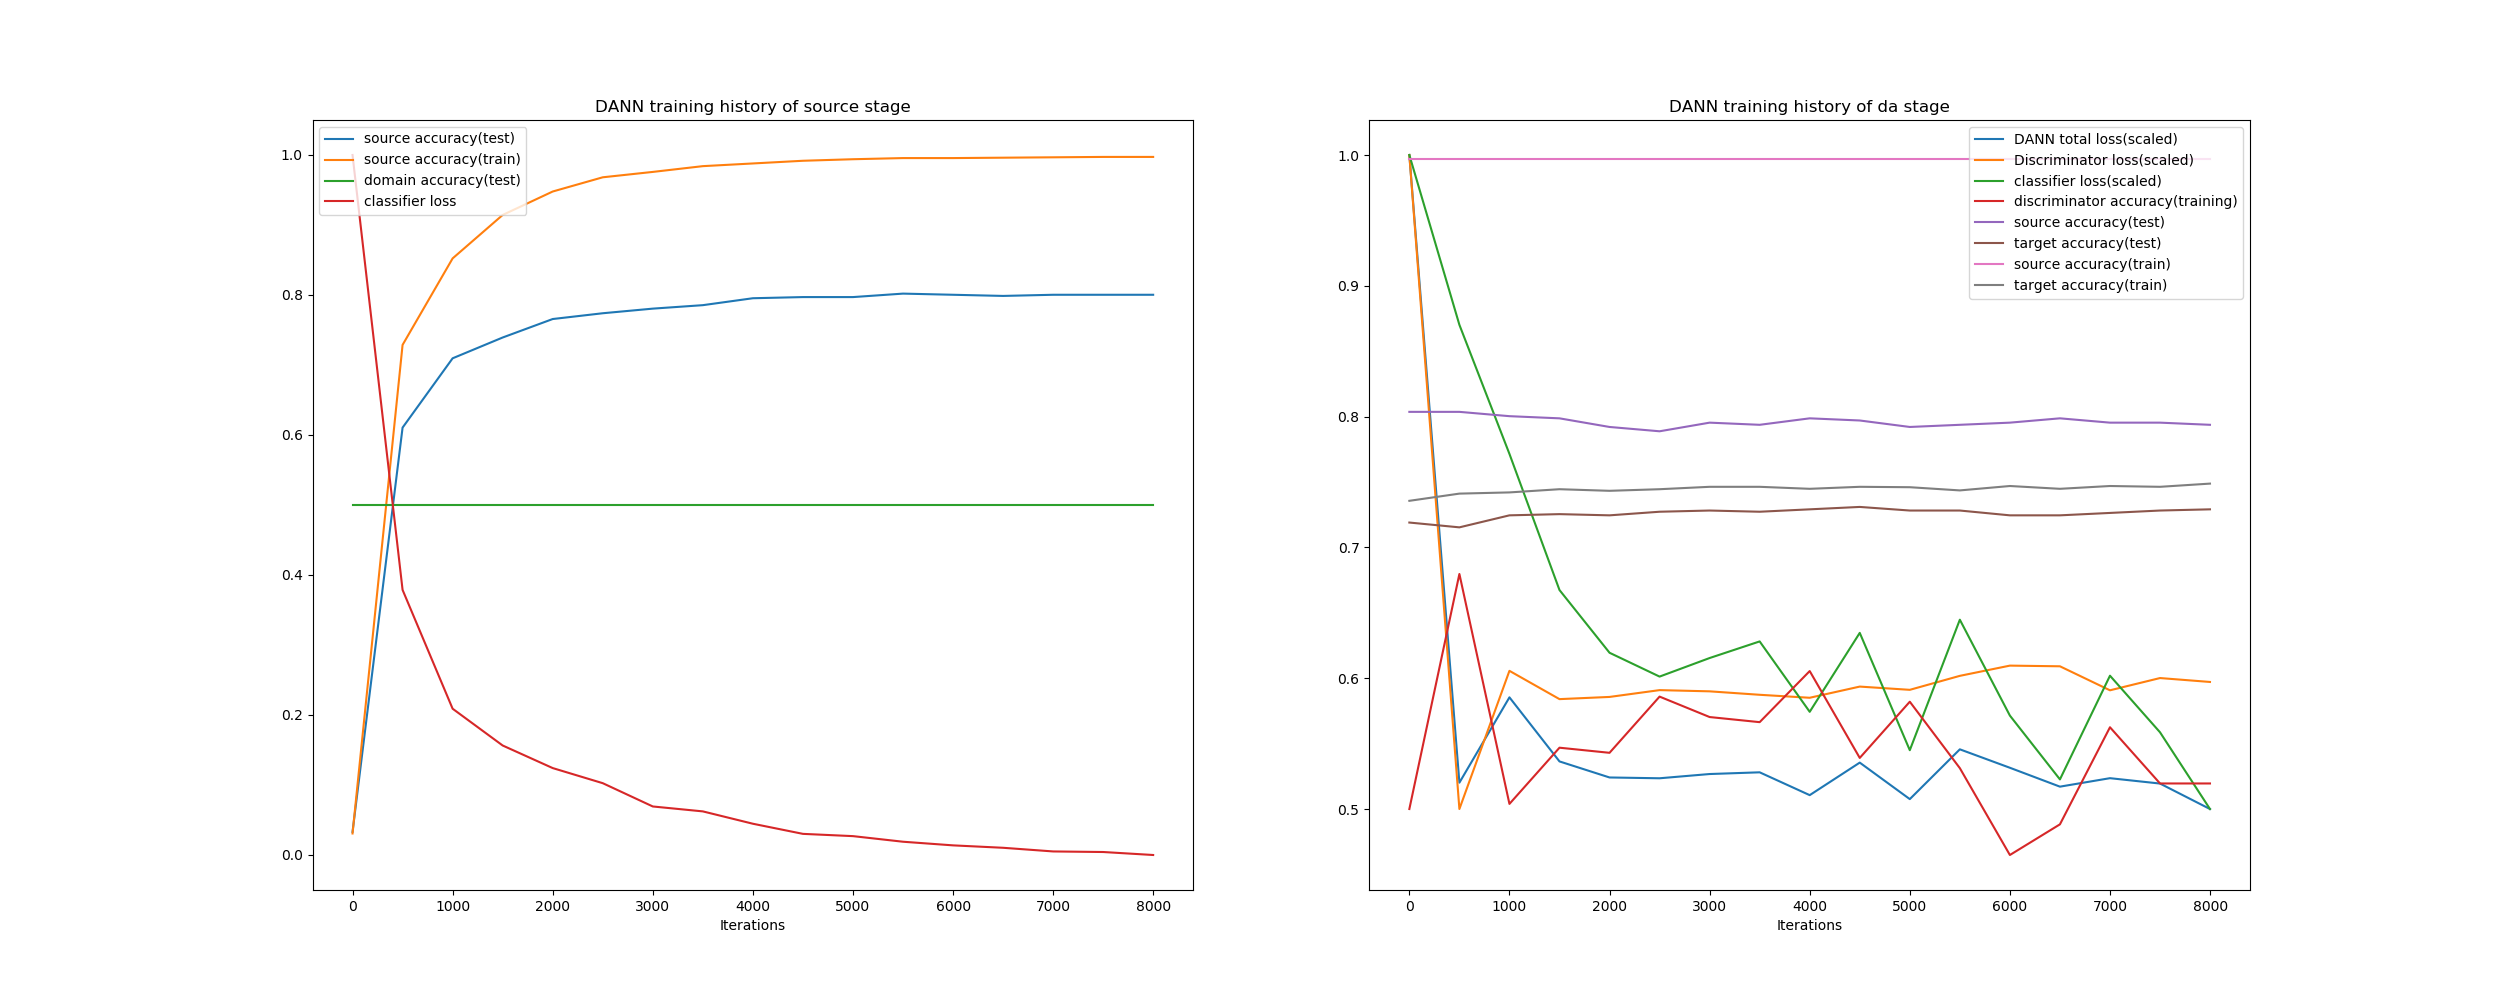
\includegraphics[width=3.5in, height=1.5in]{Ldann/std_A2R/dann.png}
\end{minipage}%
\caption{Visualization of DANN ExA Result}\label{fig:ExA2}
\end{figure*}

\subsection{Summary of Results}
In this part, we present a summary of accuracies using different approaches for comparison, as illustrated in table \ref{tab:ex_sum}. All of the accuracies are the best achieved with the indicated approach, no matter what configuration of hyper-parameters is. Baselines are provided. "Baseline-Deep" indicates the accuracies achieved using classification network trained only with source domain samples to classify target domain samples. Both test and training accuracies are provided if $X_t$ is splited so. Actually, we only did so in ADDA and DANN's experiments and take all $X_t$ for training of other domain adaptation models. It is not always necessary to split $X_t$ into training and test set since domain adaptation is usually assuming $X_t$ as the test set that is subject to a distribution different from $X_s$. Therefore, it should be use training accuracies of ADDA and DANN, $M_t(X^{tr}_t)$, for comparison.

Headers, A2R, C2R and P2R of table \ref{tab:ex_sum}, indicate we transfer respectively from Art, Clipboard and Product domain into RealWorld domain. Compared with baselines, we can decide TCA, JDA and ADDA do well in domain adaptation, improving the accuracies by at least 0.01 in all of the three tasks. On the contrary, CORAL, KMM do not perform so well. And it should be noticed that ADDA outperforms all other methods in general.
 \begin{table}[h]
	\centering
	\caption{Summary of Experiment Results}
	\label{tab:ex_sum}
	\begin{tabular}{cccc}
		\hline
		Approach & A2R & C2R & P2R\\
		\hline
		\hline
		Baseline-SVM &  0.7473 & 0.6511 & 0.7296 \\
        Baseline-KNN &  0.6580 & 0.5864 & 0.6957 \\
        Baseline-Deep &  0.7313 & 0.6561 & 0.7313 \\
		TCA &  0.7604 & 0.6693* & 0.7429 \\
		CORAL &  0.7450 &  0.6514 & 0.7310 \\
        KMM &  0.7471 &  0.6518 & 0.7299 \\
        JDA &  0.7530 &  0.6656 & 0.7482 \\
        DaNN &  0.7599 &  0.6617 & 0.7381 \\
        ADDA-Test &  0.7354 &  0.6636 & 0.7353 \\
        ADDA-Training &  0.7621* &  0.6646 & 0.7556* \\
        DANN-Test &  0.7301 &  0.6547 & 0.7392 \\
        DANN-Training &  0.7488 &  0.6683 & 0.7411 \\
		\hline
	\end{tabular}
\end{table}


\section{Discussions}
\subsection{Review of Maximum Mean Discrepancy}
For TCA, JDA, KMM and DaNN, we find that they all use the Maximum Mean Discrepancy(MMD) measure as a tool to reduce the distribution mismatch between the source and target domains in the latent space. MMD can be explained as a statistic which means the difference between the mean function values on two samples drawn for two distributions $p$ and $q$ respectively. When MMD is large, the $p$ and $q$ are likely different.

Let $p$ and $q$ be distributions defined on a domain $\mathcal{X}$. Given observations $X := \left\{x_{1}, \dots, x_{m}\right\}$ and $Y :=\left\{y_{1}, \dots, y_{n}\right\}$. And let $\mathfrak{F}$ be a class of functions $f : x \rightarrow \mathbb{R}$. Then we can define the maximum mean discrepancy(MMD) and its empirical estimate as:
\begin{equation}
\operatorname{MMD}[\mathcal{F}, p, q] :=\sup _{f \in \mathcal{F}}\left(\mathbf{E}_{x \sim p}[f(x)]-\mathbf{E}_{y \sim q}[f(y)]\right)
\end{equation}

\begin{equation}
\operatorname{MMD}[\mathcal{F}, X, Y] :=\sup _{f \in \mathcal{F}}\left(\frac{1}{m} \sum_{i=1}^{m} f\left(x_{i}\right)-\frac{1}{n} \sum_{i=1}^{n} f\left(y_{i}\right)\right)
\end{equation}

Take RKHS into consideration, we can get a new empirical of MMD:
\begin{equation}
\begin{split}
 \operatorname{MMD} & [\mathcal{F}, X, Y]= \\
& [\frac{1}{m^{2}} \sum_{i, j=1}^{m} k\left(x_{i}, x_{j}\right)-\frac{2}{m n} \sum_{i, j=1}^{m, n} k\left(x_{i}, y_{j}\right)+ \\
& \frac{1}{n^{2}} \sum_{i, j=1}^{n} k\left(y_{i}, y_{j}\right)]^{\frac{1}{2}}
\end{split}
\end{equation}
This form is more easily to do computation and most domain adaptation methods use this form to calculate MMD.

Based on the same basic idea, though, these approaches are quite different. TCA minimizes MMD of distribution of unlabeled source and target data directly using kernel trick; JDA tries to minimize MMD of differences of joint distributions of labeled source and target data; KMM combines MMD into SVM loss sophisticatedly; DaNN adds MMD to network loss to train a classifier. And the performances also differ. In our experiments, TCA, which directly reduces MMD, performs best among all of these four.

\subsection{Problems of Network Design}
No matter which deep model we applied, severe overfitting occurs when training the classifier. Take ADDA for example, $Ac(M_s(X^{tr}_s))$ are always greater than $Ac(M_s(X^{te}_s))$ by about 0.15. We tried dropping out some neurons and increases L2 regularization constraint, but these measures do not ease overfitting but brings negative effects on $Ac(M_s(X^{te}_s))$.

Besides, specifically for ADDA, we found the discriminator can really grow too capable to distinguish $X_s$ and $X_t$. We can design a more complicated and powerful $M$ to deceive the discriminator, of course. But a more complicated $M$ can also bring difficulties for the classification work.

And, it should be noticed that the visualization doesn't show an obvious effect after domain adaptation and the performance gain using domain adaptation is also poor, $g^{te} < 0.015, g^{tr} < 0.035$. We think there can still be room for improvement.

\subsection{Theory of Batch Normalization}
From ADDA experiments, we can see batch normalization really make a learning process converge easier and faster(refer to figure \ref{fig:Ex3} and \ref{fig:ExA}). Method of batch normalization is proposed in Sergey Ioffe et al.'s work \cite{BN1}.

Batch normalization is used before activation function applied to the output of a layer. Assuming that every batch fed for the network satisfy a distribution $d_0(x, \theta_0)$, with the network forwarding, the distribution changes into $d_1(x, \theta_1), d_2(x, \theta_2), \cdots, d_i(x, \theta_i)$ and goes far away from the Y-axis, which is named internal covariate shift in Sergey Ioffe et al.'s work\cite{BN1}, as illustrated in the left subfigure of figure \ref{fig:BN_theorem1}. Supposing sigmoid function is used for activation, the gradients will become flat, making it difficult for update of parameters using SGD method.
\begin{figure}
  \centering
  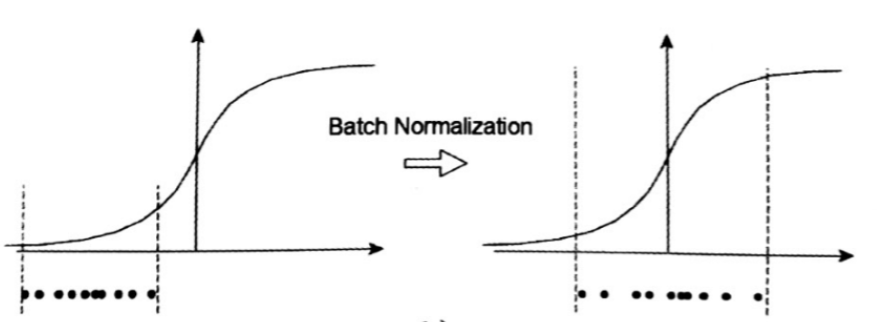
\includegraphics[width=.4\textwidth]{LBN_theorem1.jpg}
  \caption{Internal Covariate Shift and Batch Normalization}
  \label{fig:BN_theorem1}
\end{figure}
As a result, we normalize the output $\mathbf{x}$ to normal distribution. But, that is not done because distribution of $\mathbf{x}$ is constrained to Gaussian. So a linear transformation, scale and shift, is applied to keep the feature of $\mathbf{x}$'s original distribution. Intuitively, batch normalization aims to pull $\mathbf{x}$ back to where gradients of the activation function work to accelerate the convergence process.

\subsection{Ceiling Caused by Domain Uncorrelation}
It is a fact that no matter which method is used, for given pair source and target domains, whether A2R, C2R or P2R, the resulted classification performances on target data do not differ that much if KNN baselines are ignored. KNN is not suitable for the given features's classification. The classification accuracy differences are always within $0.03$ for a given pair of source and target domains.

This is likely to be limited by correlation of the two domains. We are always assuming data from the source and target domains are highly correlated. But the assumption is not necessarily true in reality. There can always be some kind of uncorrelation between two domains. And such uncorrelation can lead a ceiling of performances of domain adaptation's methods.


\section{Conclusion}
We use seven methods of domain adaptation on deep features of OfficeHome-Dataset and summarize differences and similarities of these approaches' theories and performances.

We can make a simple summary over theories of the methods. TCA, JDA, KMM and DaNN, reduce MMD; DaNN, ADDA and DANN, use neural networks; CORAL, interestingly, reduces covariance difference; KMM and DaNN combine domain adaptation and classification together(so adapted features are not accessible); ADDA and DANN apply adversarial loss for domain adaptation.

To our disappointment, compared with baselines, these methods of domain adaptation failed to bring a great improvement such that classification accuracies on target data reaches that on source data. But, the methods do help in some degree, giving an accuracy increasing of at least $0.01$ and at most $0.03$. Different methods's performances vary, too, according to summary of table \ref{tab:ex_sum}.

It is a fact that no matter which method is used, for given source and target domain, whether A2R, C2R or P2R, the resulted classification performances on target data do not differ that much. This is likely to be limited by correlation of the two domains. In other words, uncorrelation of the source and target domains also brings difficulties for work of domain adaptation.

\section*{References}

\begin{thebibliography}{00}
\bibitem{ADDA1} Eric Tzeng, Judy Hoffman, Kate Saenko and Trevor Darrel, ``Adversarial Discriminative Domain Adaptation''.
\bibitem{DANN1} Yaroslav Ganin, Evgeniya Ustinova, Hana Ajakan, Pascal Germain, Hugo Larochelle, Francois Laviolette,
    Mario Marchand, Victor Lempitsky, ``Domain-Adversarial Training of Neural Networks''.
\bibitem{BN1} Sergey Ioffe, Christian Szegedy, ``Batch Normalization: Accelerating Deep Network Training by Reducing Internal Covariate Shift''.
\bibitem{TCA} Pan, Sinno Jialin, et al. "Domain adaptation via transfer component analysis." IEEE Transactions on Neural Networks 22.2 (2010): 199-210.
\bibitem{CORAL} Sun, Baochen, Jiashi Feng, and Kate Saenko. "Return of frustratingly easy domain adaptation." Thirtieth AAAI Conference on Artificial Intelligence. 2016.
\bibitem{KMM} Huang, Jiayuan, et al. "Correcting sample selection bias by unlabeled data." Advances in neural information processing systems. 2007.
\bibitem{JDA} Long, Mingsheng, et al. "Transfer feature learning with joint distribution adaptation." Proceedings of the IEEE international conference on computer vision. 2013.
\bibitem{DaNN} Ghifary, Muhammad, W. Bastiaan Kleijn, and Mengjie Zhang. "Domain adaptive neural networks for object recognition." Pacific Rim international conference on artificial intelligence. Springer, Cham, 2014.
\end{thebibliography}


\begin{figure*}[htb]

\centering
\begin{minipage}[t]{0.26\textwidth}
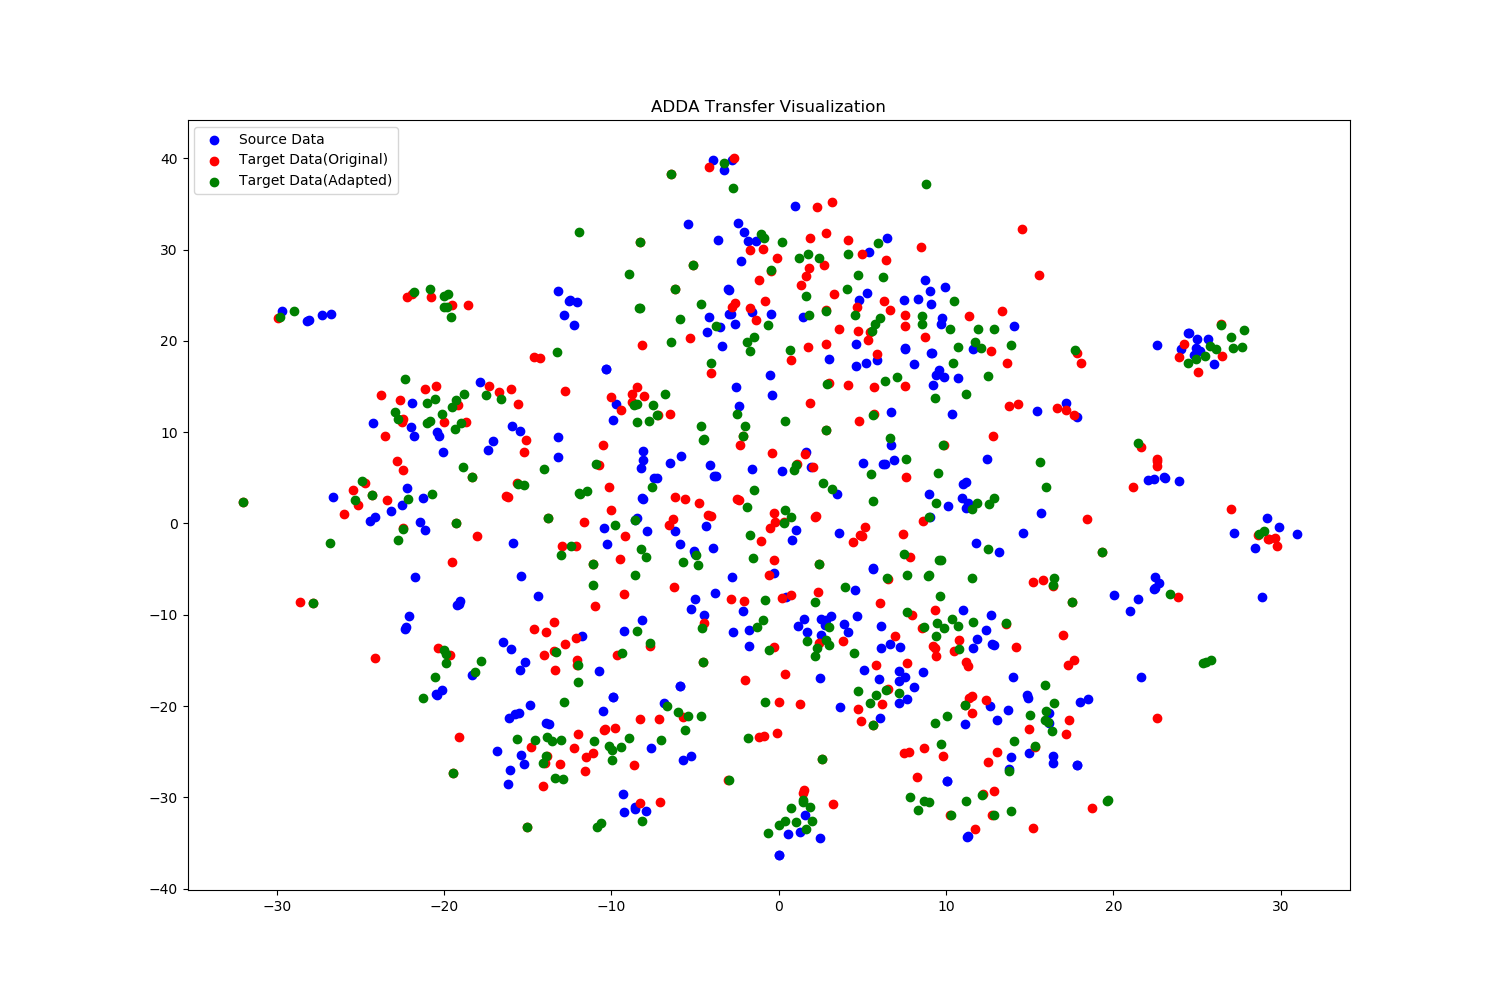
\includegraphics[width=1.6in, height=1.5in]{Ladda/std_C2R/ADDA_visual.png}
\end{minipage}%
\begin{minipage}[t]{0.26\textwidth}
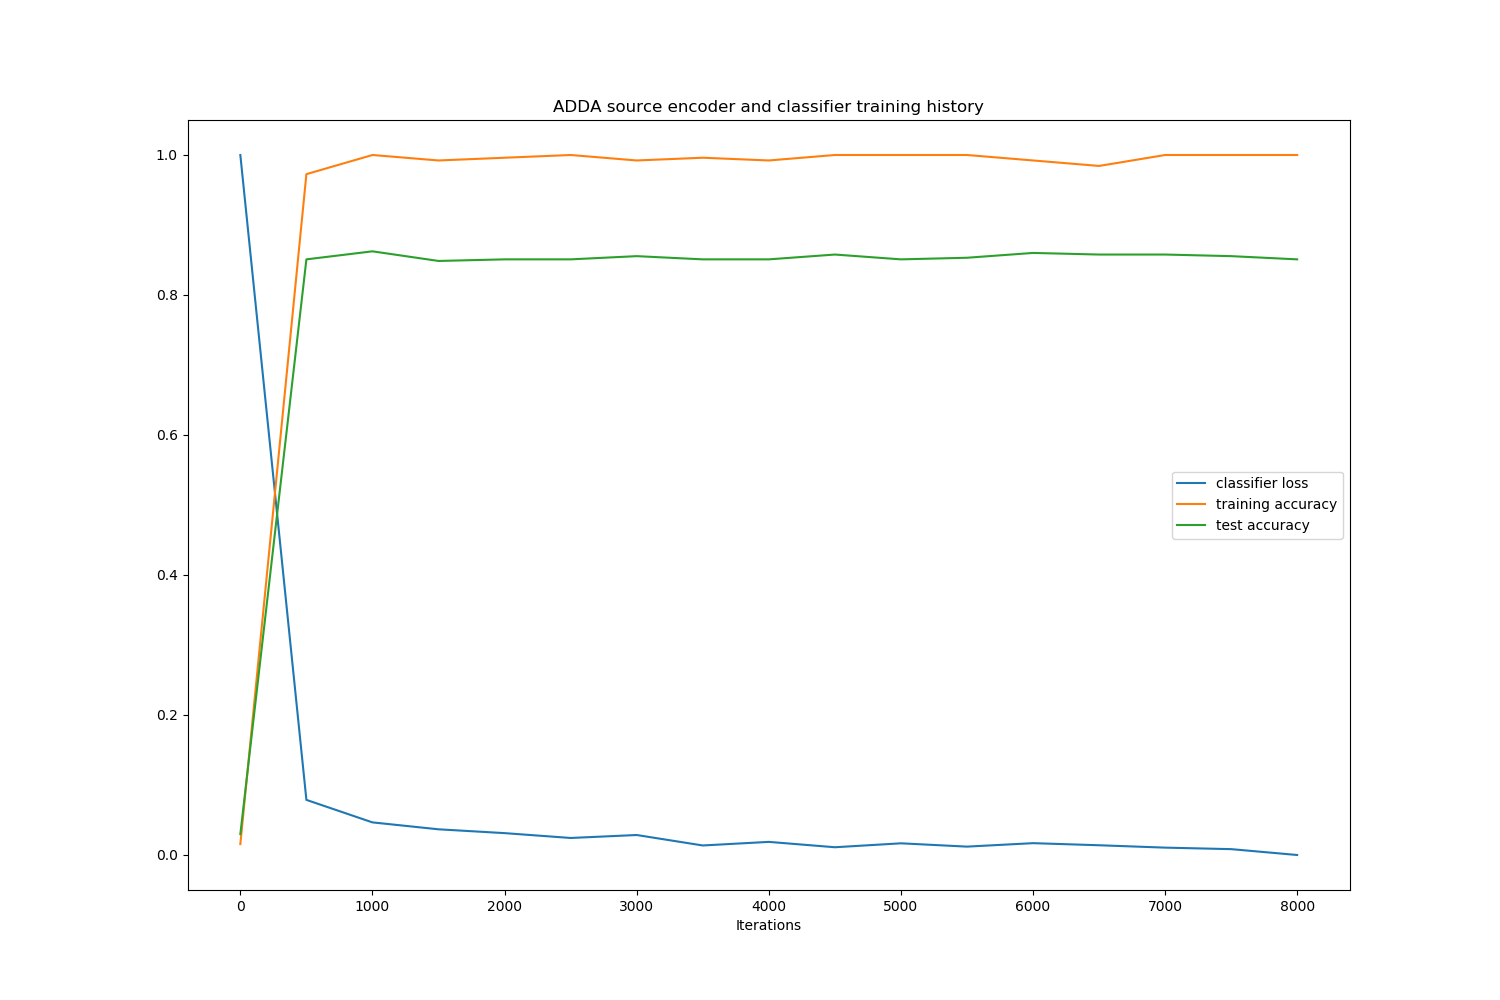
\includegraphics[width=1.6in, height=1.5in]{Ladda/std_C2R/clf.png}
\end{minipage}%
\begin{minipage}[t]{0.45\textwidth}
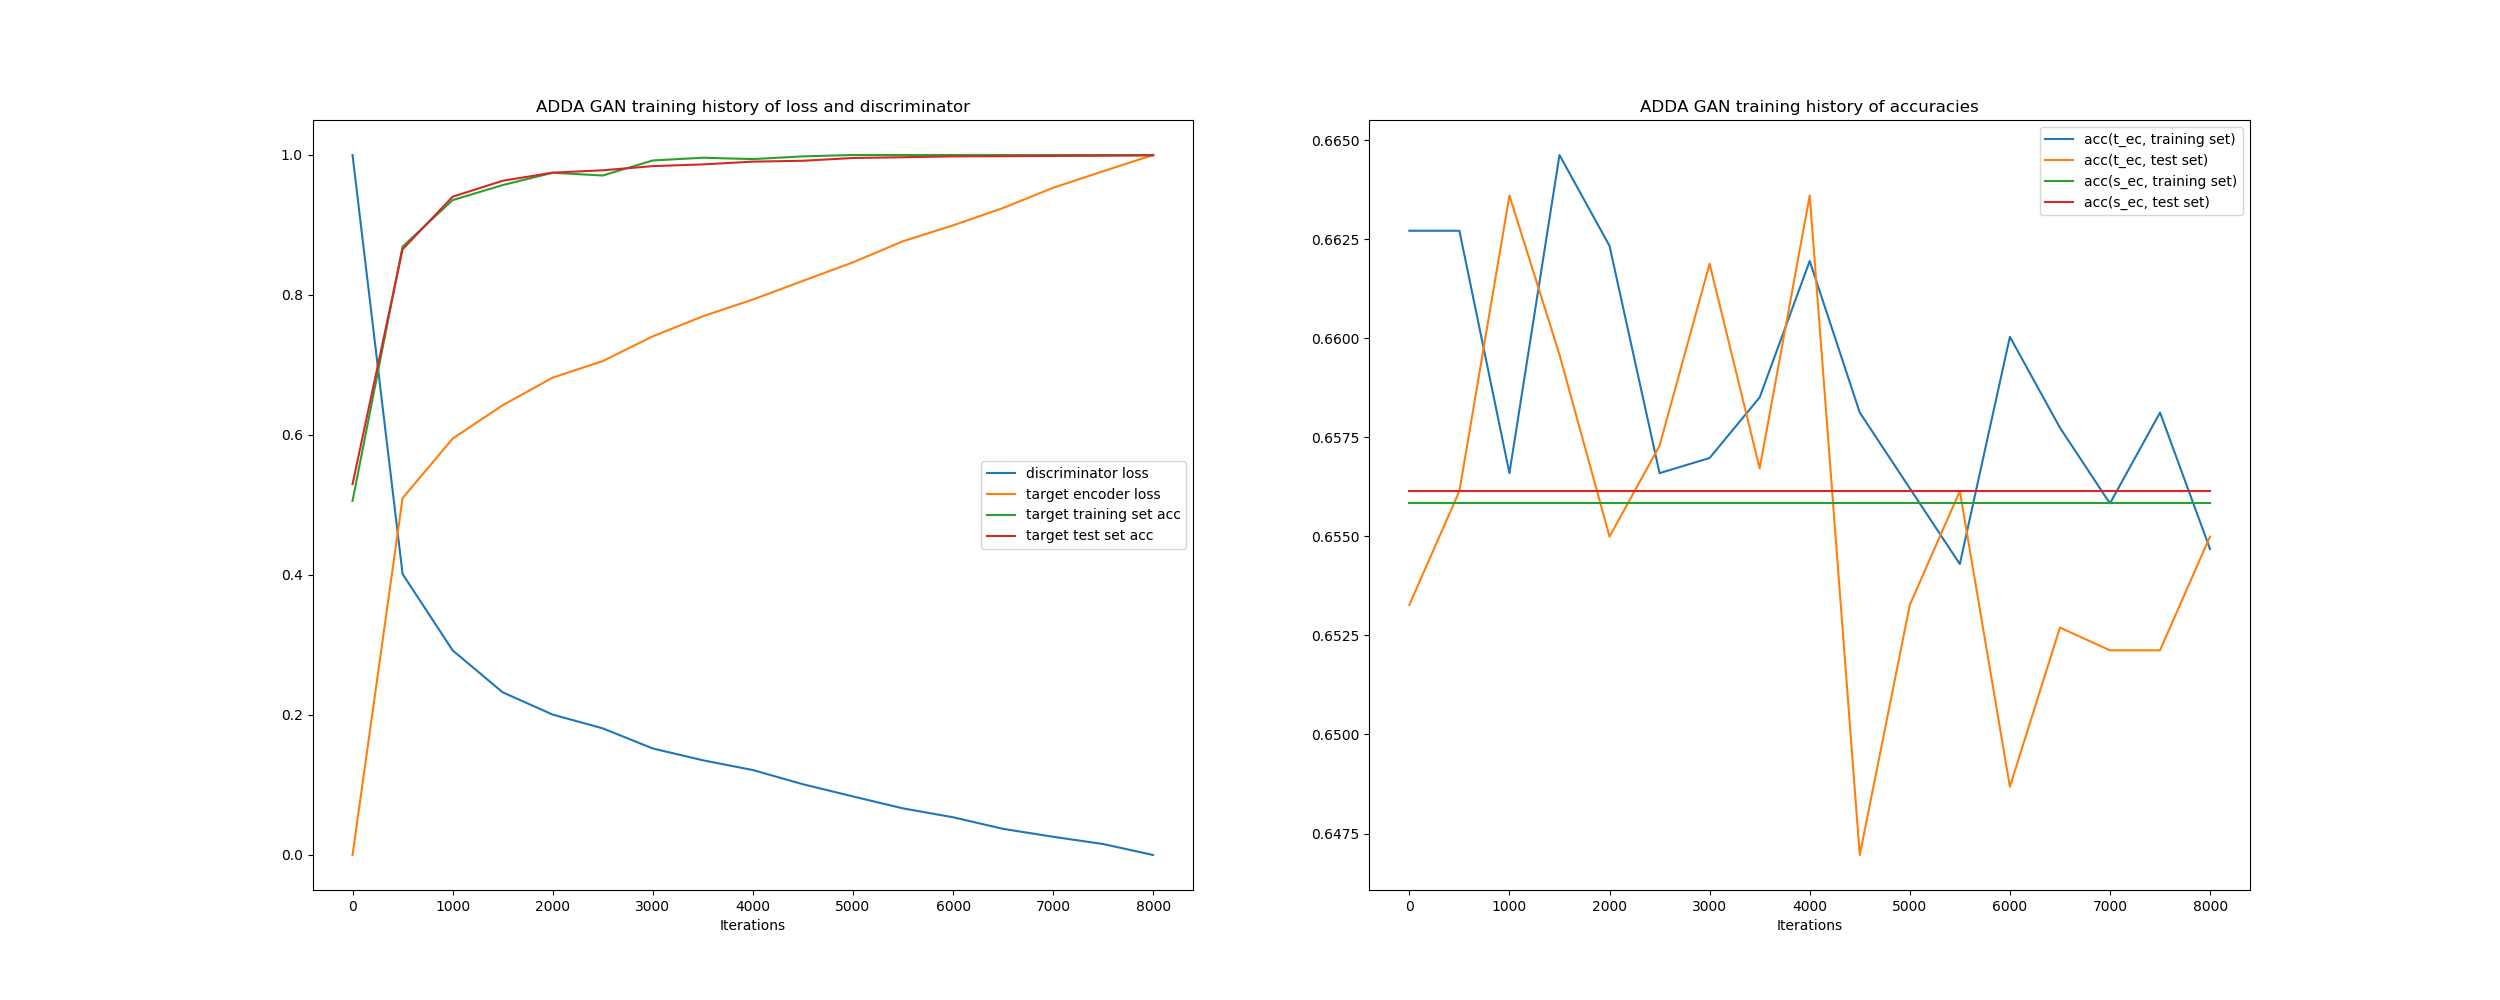
\includegraphics[width=3.5in, height=1.5in]{Ladda/std_C2R/gan.png}
\end{minipage}%
\caption{Visualization of ADDA ExC Result}\label{fig:ExC}
\end{figure*}

\begin{figure*}[htb]

\centering
\begin{minipage}[t]{0.26\textwidth}
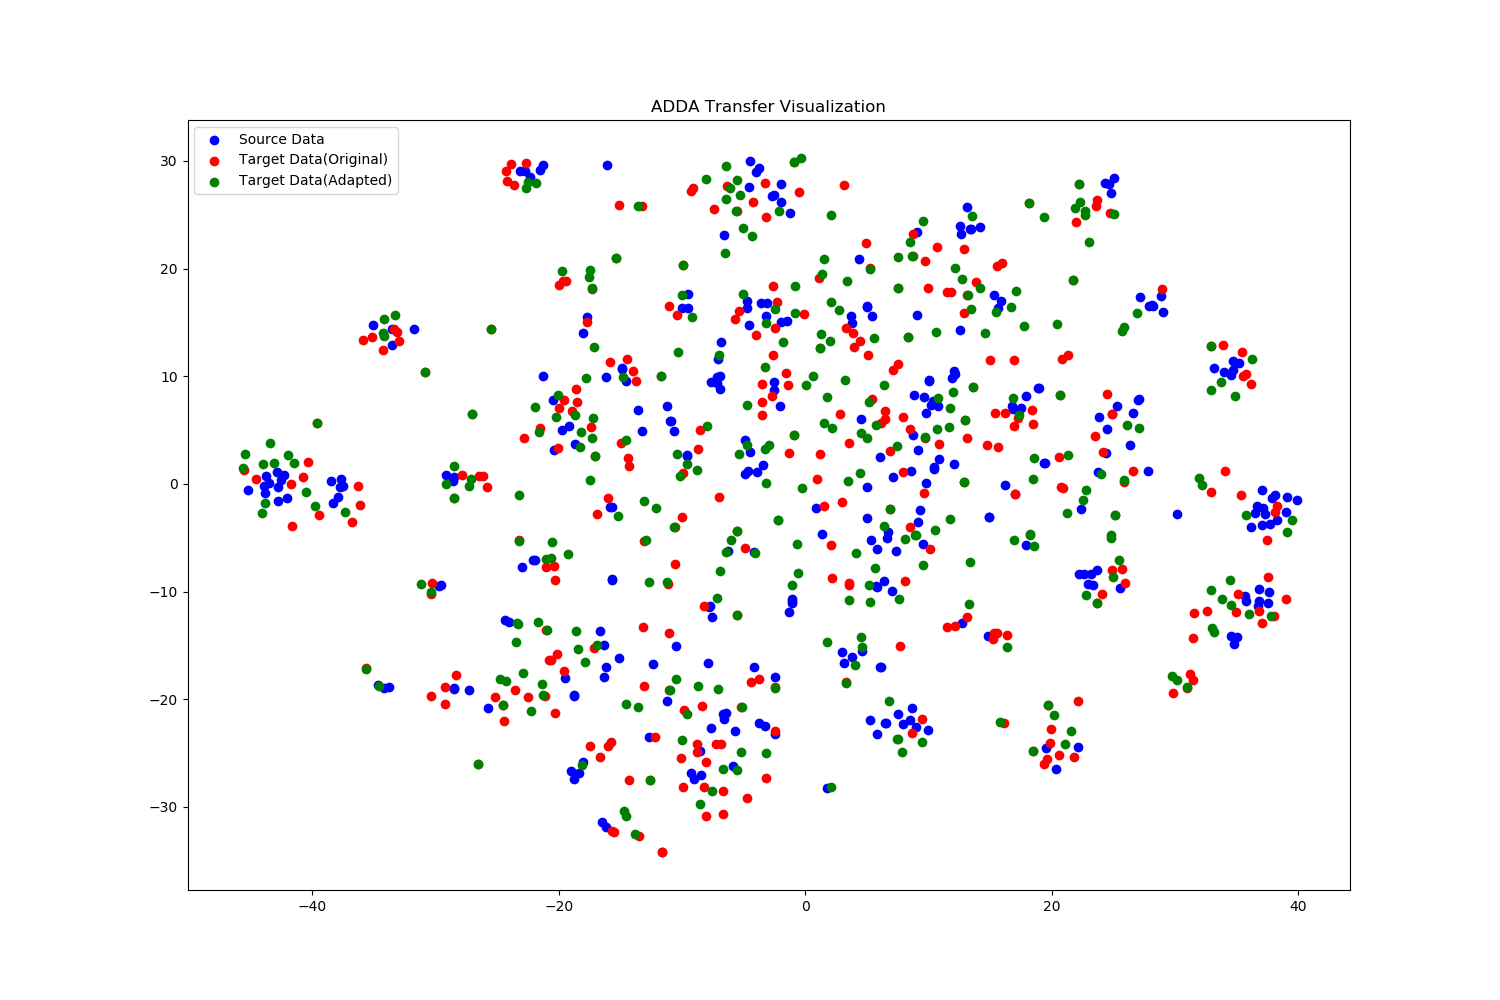
\includegraphics[width=1.6in, height=1.5in]{Ladda/std_P2R/ADDA_visual.png}
\end{minipage}%
\begin{minipage}[t]{0.26\textwidth}
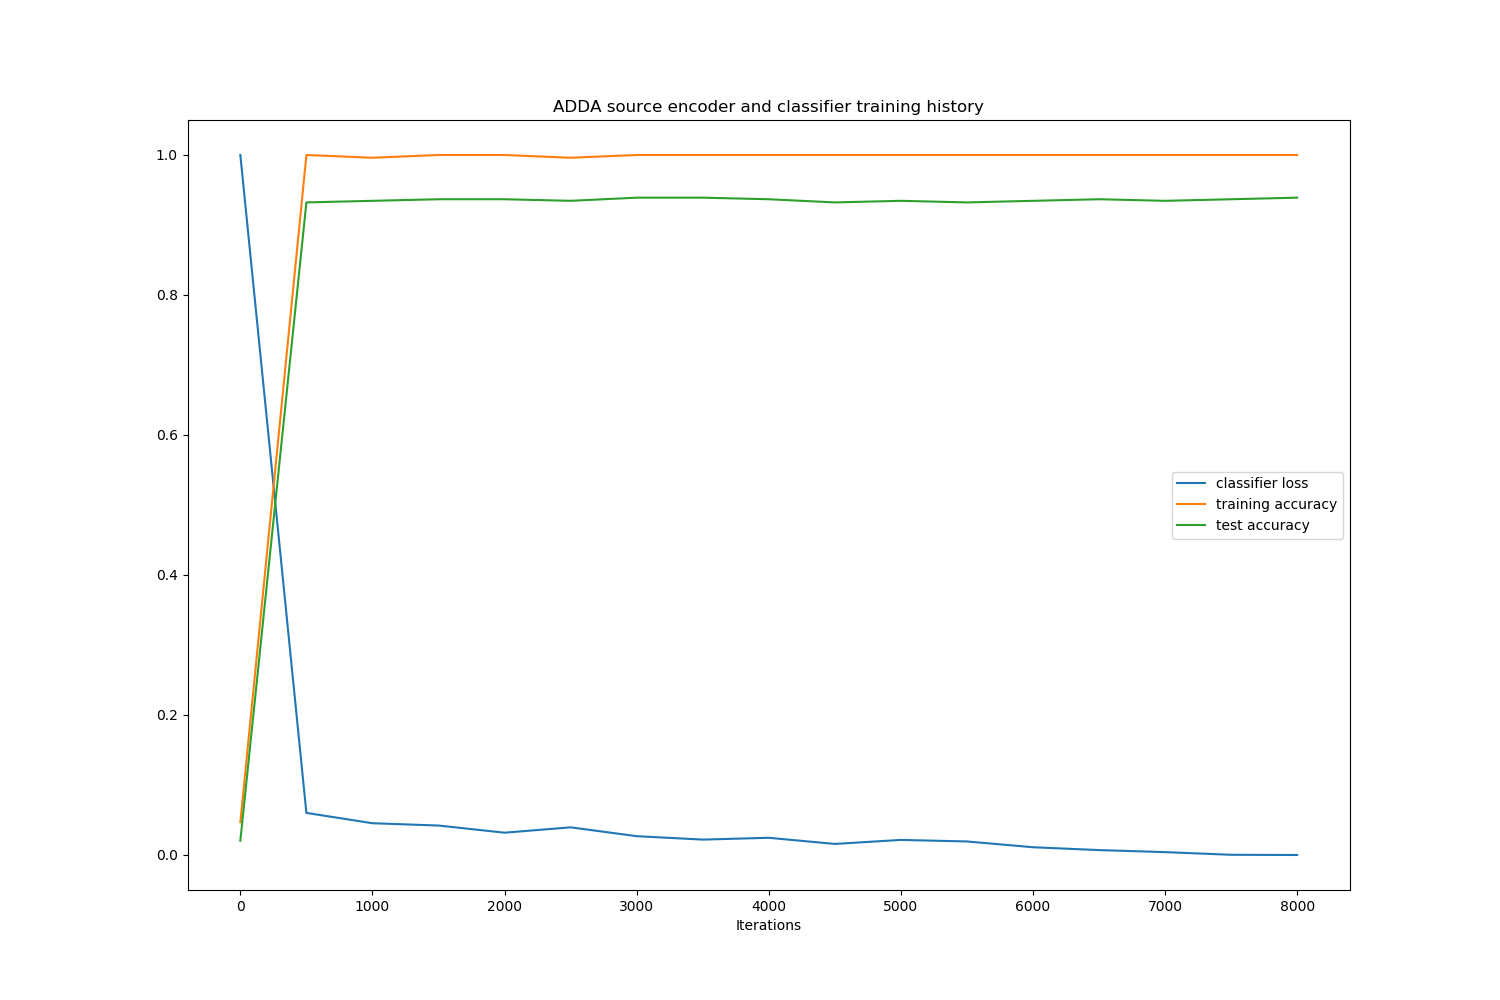
\includegraphics[width=1.6in, height=1.5in]{Ladda/std_P2R/clf.png}
\end{minipage}%
\begin{minipage}[t]{0.45\textwidth}
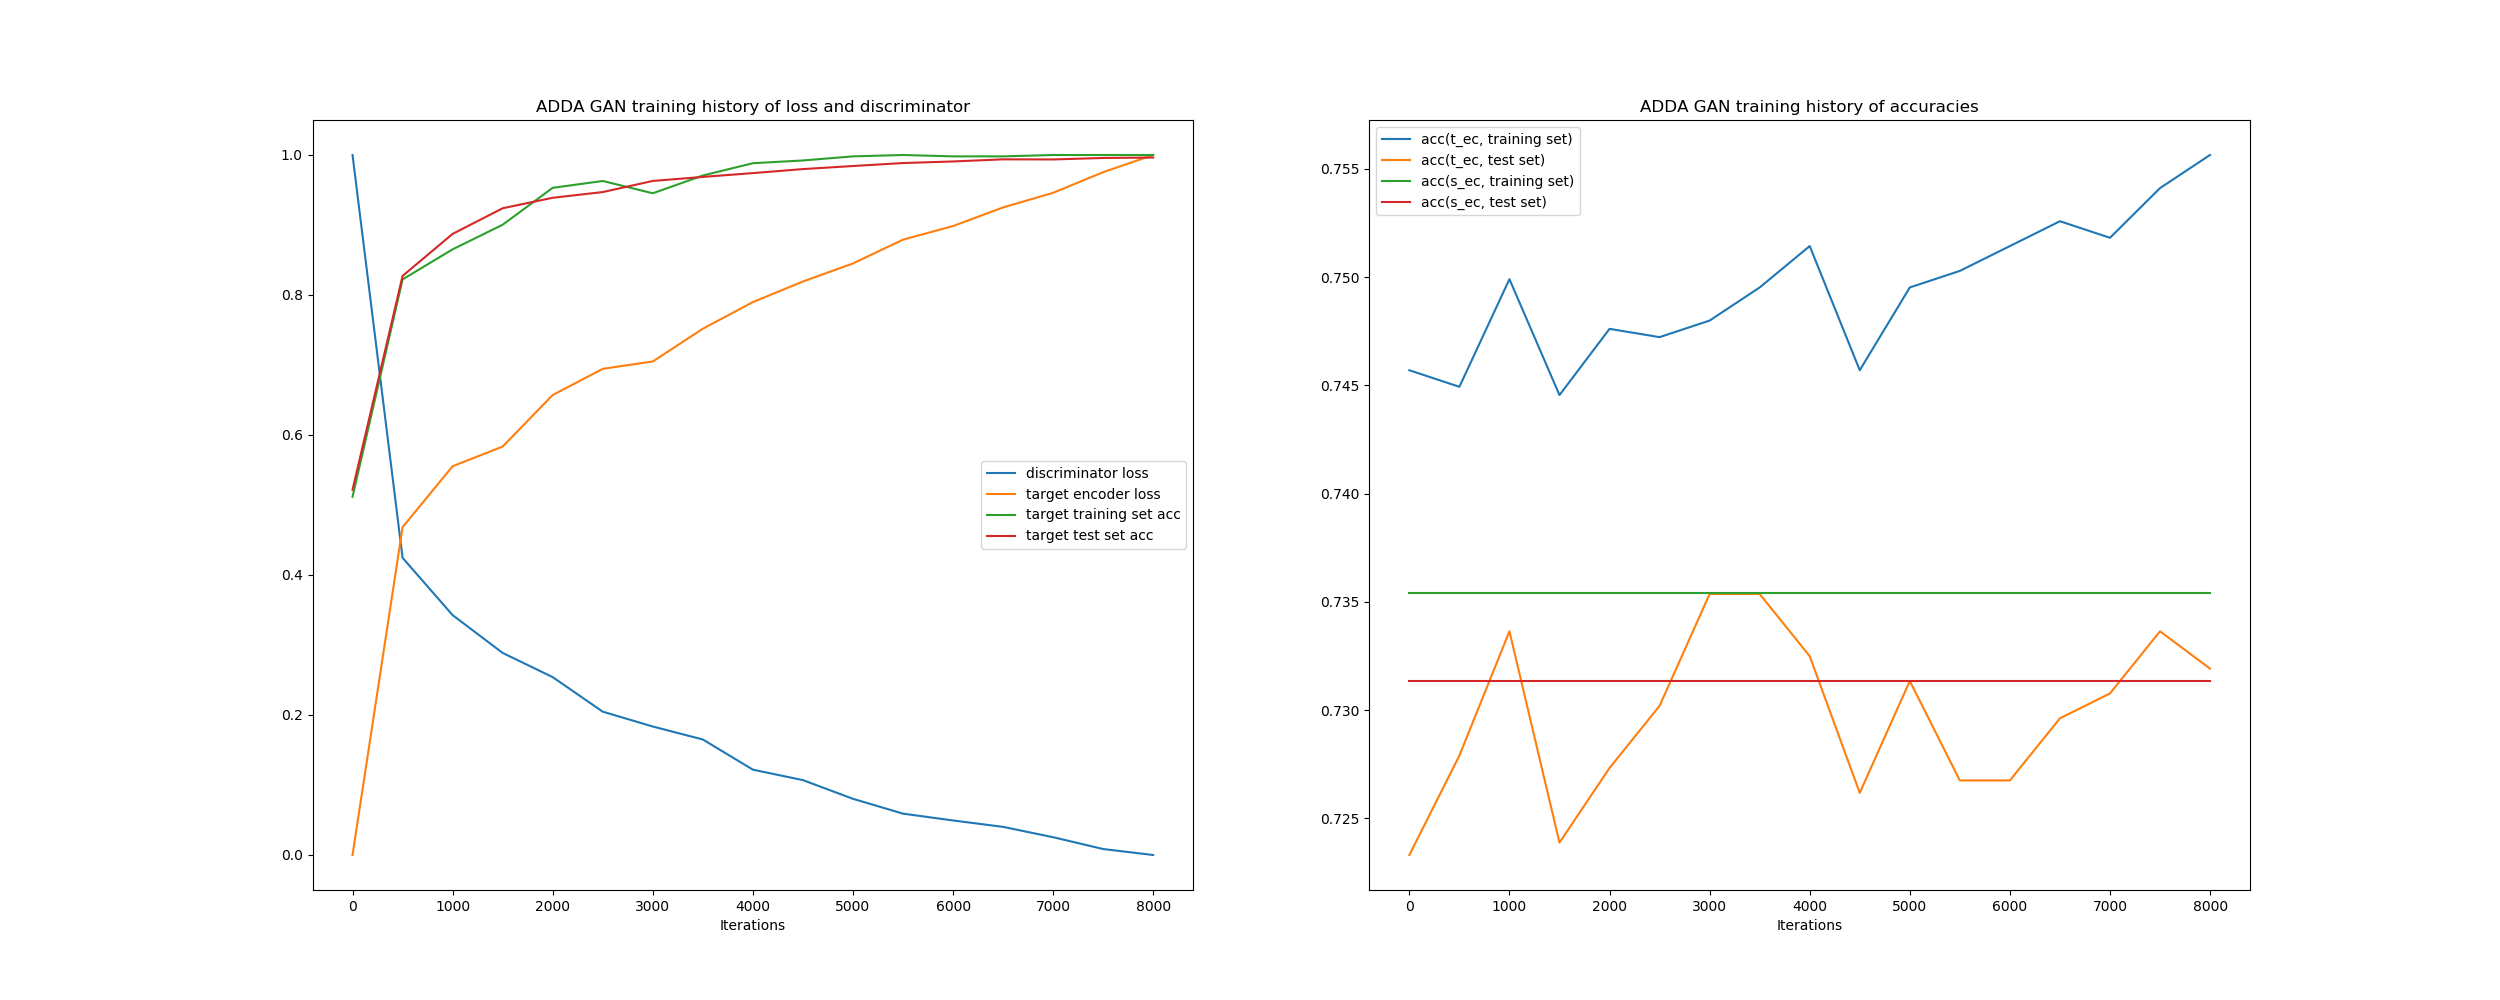
\includegraphics[width=3.5in, height=1.5in]{Ladda/std_P2R/gan.png}
\end{minipage}%
\caption{Visualization of ADDA ExP Result}\label{fig:ExP}
\end{figure*}

\begin{figure*}[htb]
\centering
\begin{minipage}[t]{0.26\textwidth}
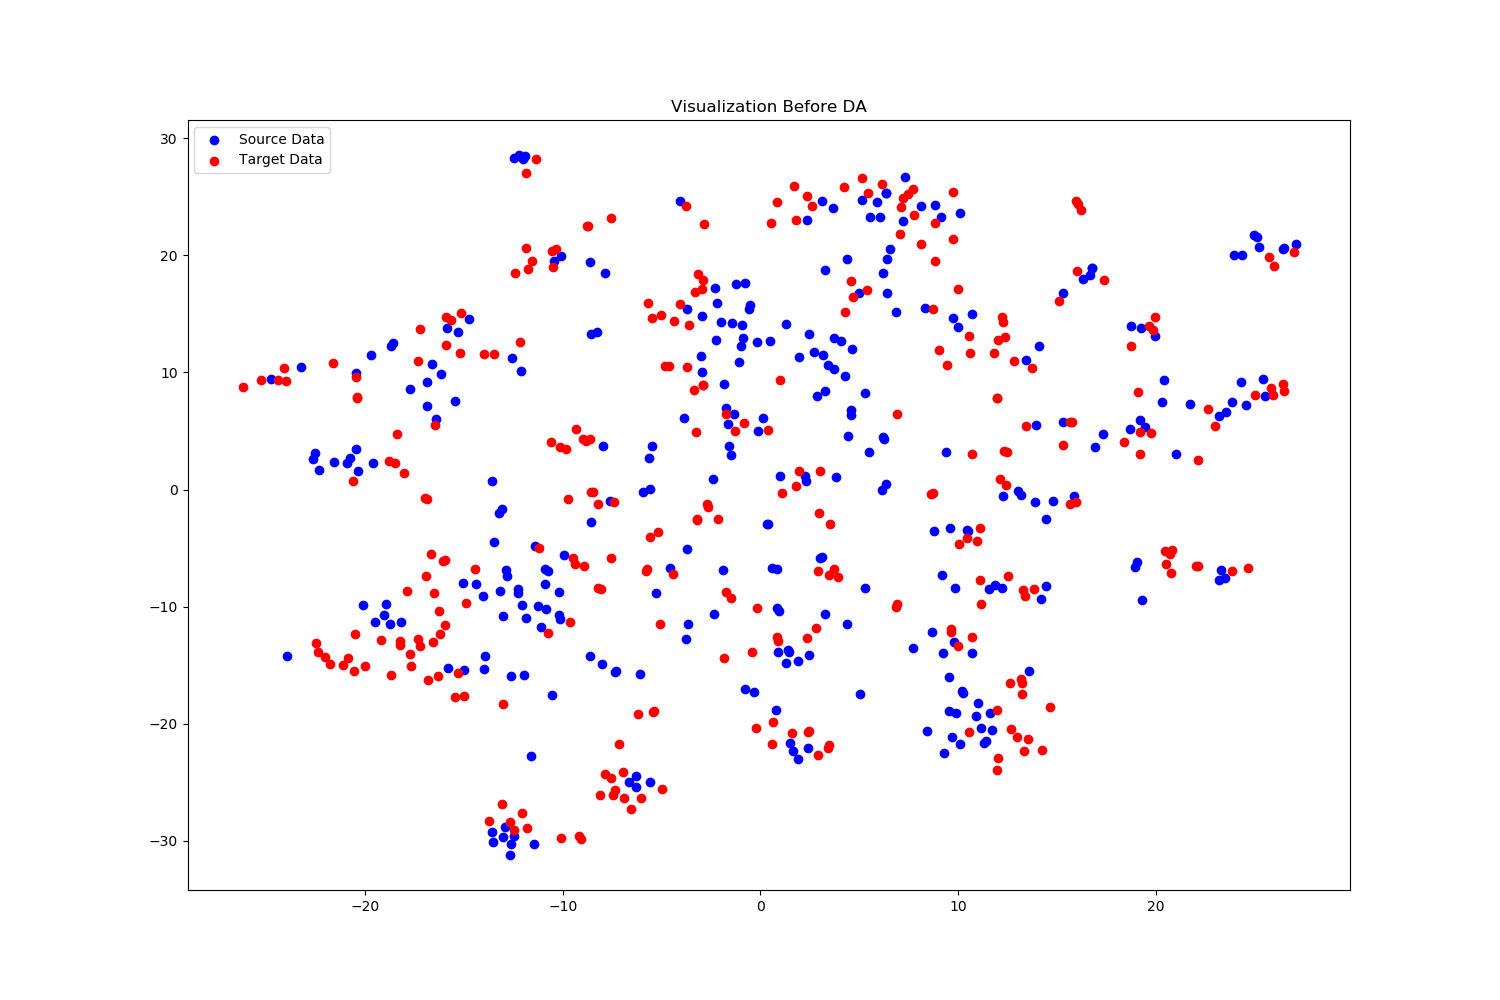
\includegraphics[width=1.6in, height=1.5in]{Ldann/std_C2R/before.png}
\end{minipage}%
\begin{minipage}[t]{0.26\textwidth}
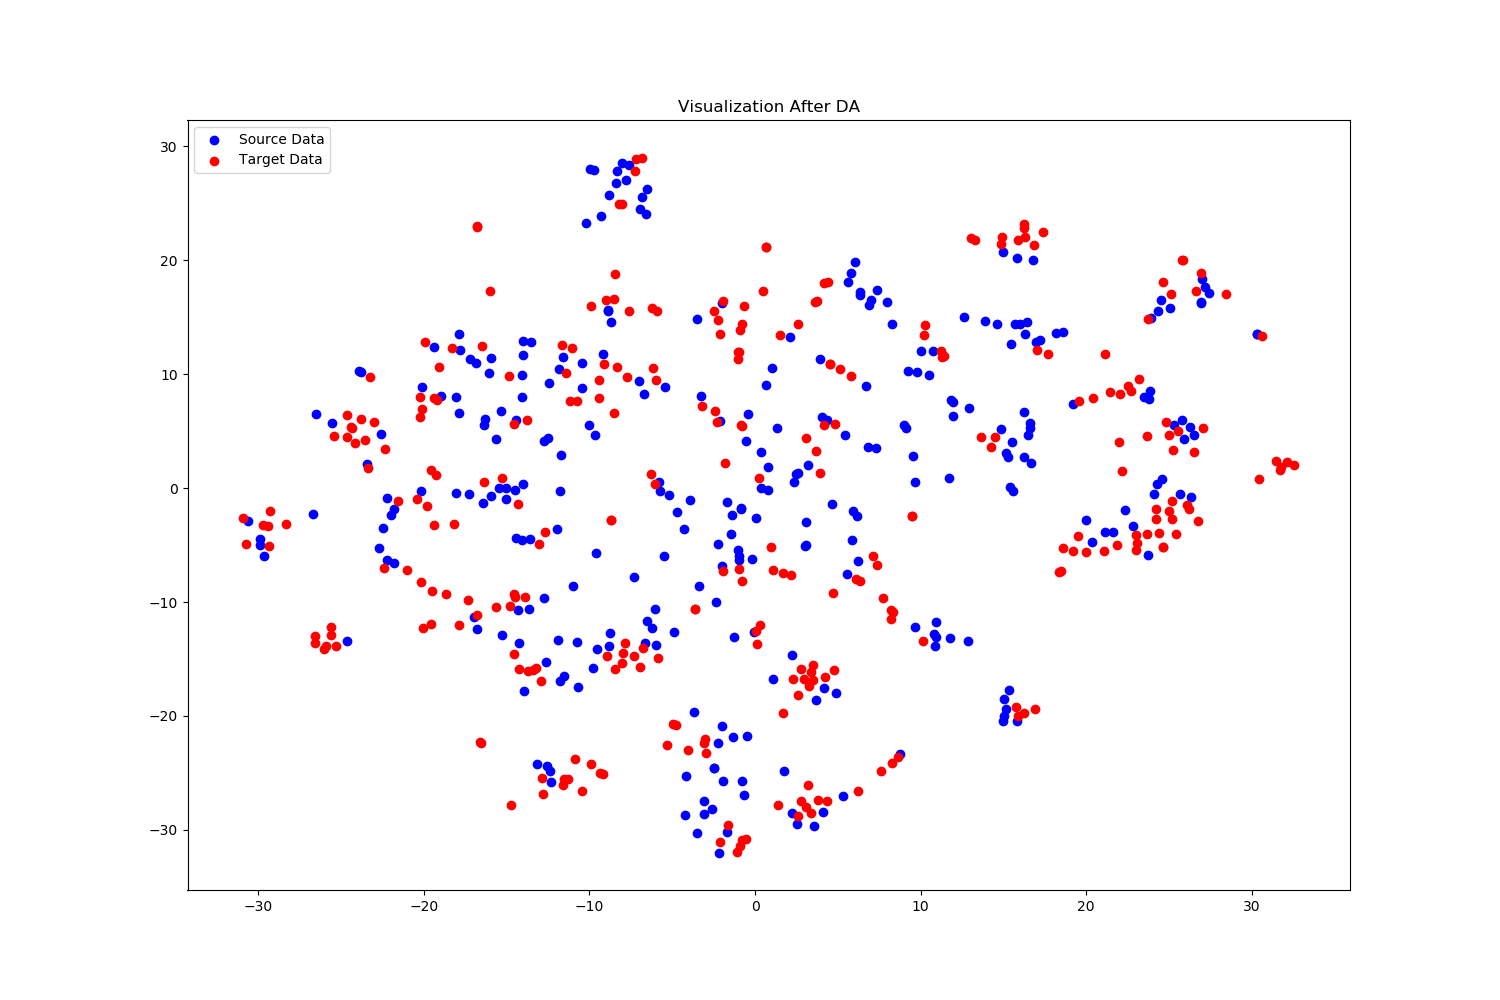
\includegraphics[width=1.6in, height=1.5in]{Ldann/std_C2R/after.png}
\end{minipage}%
\begin{minipage}[t]{0.45\textwidth}
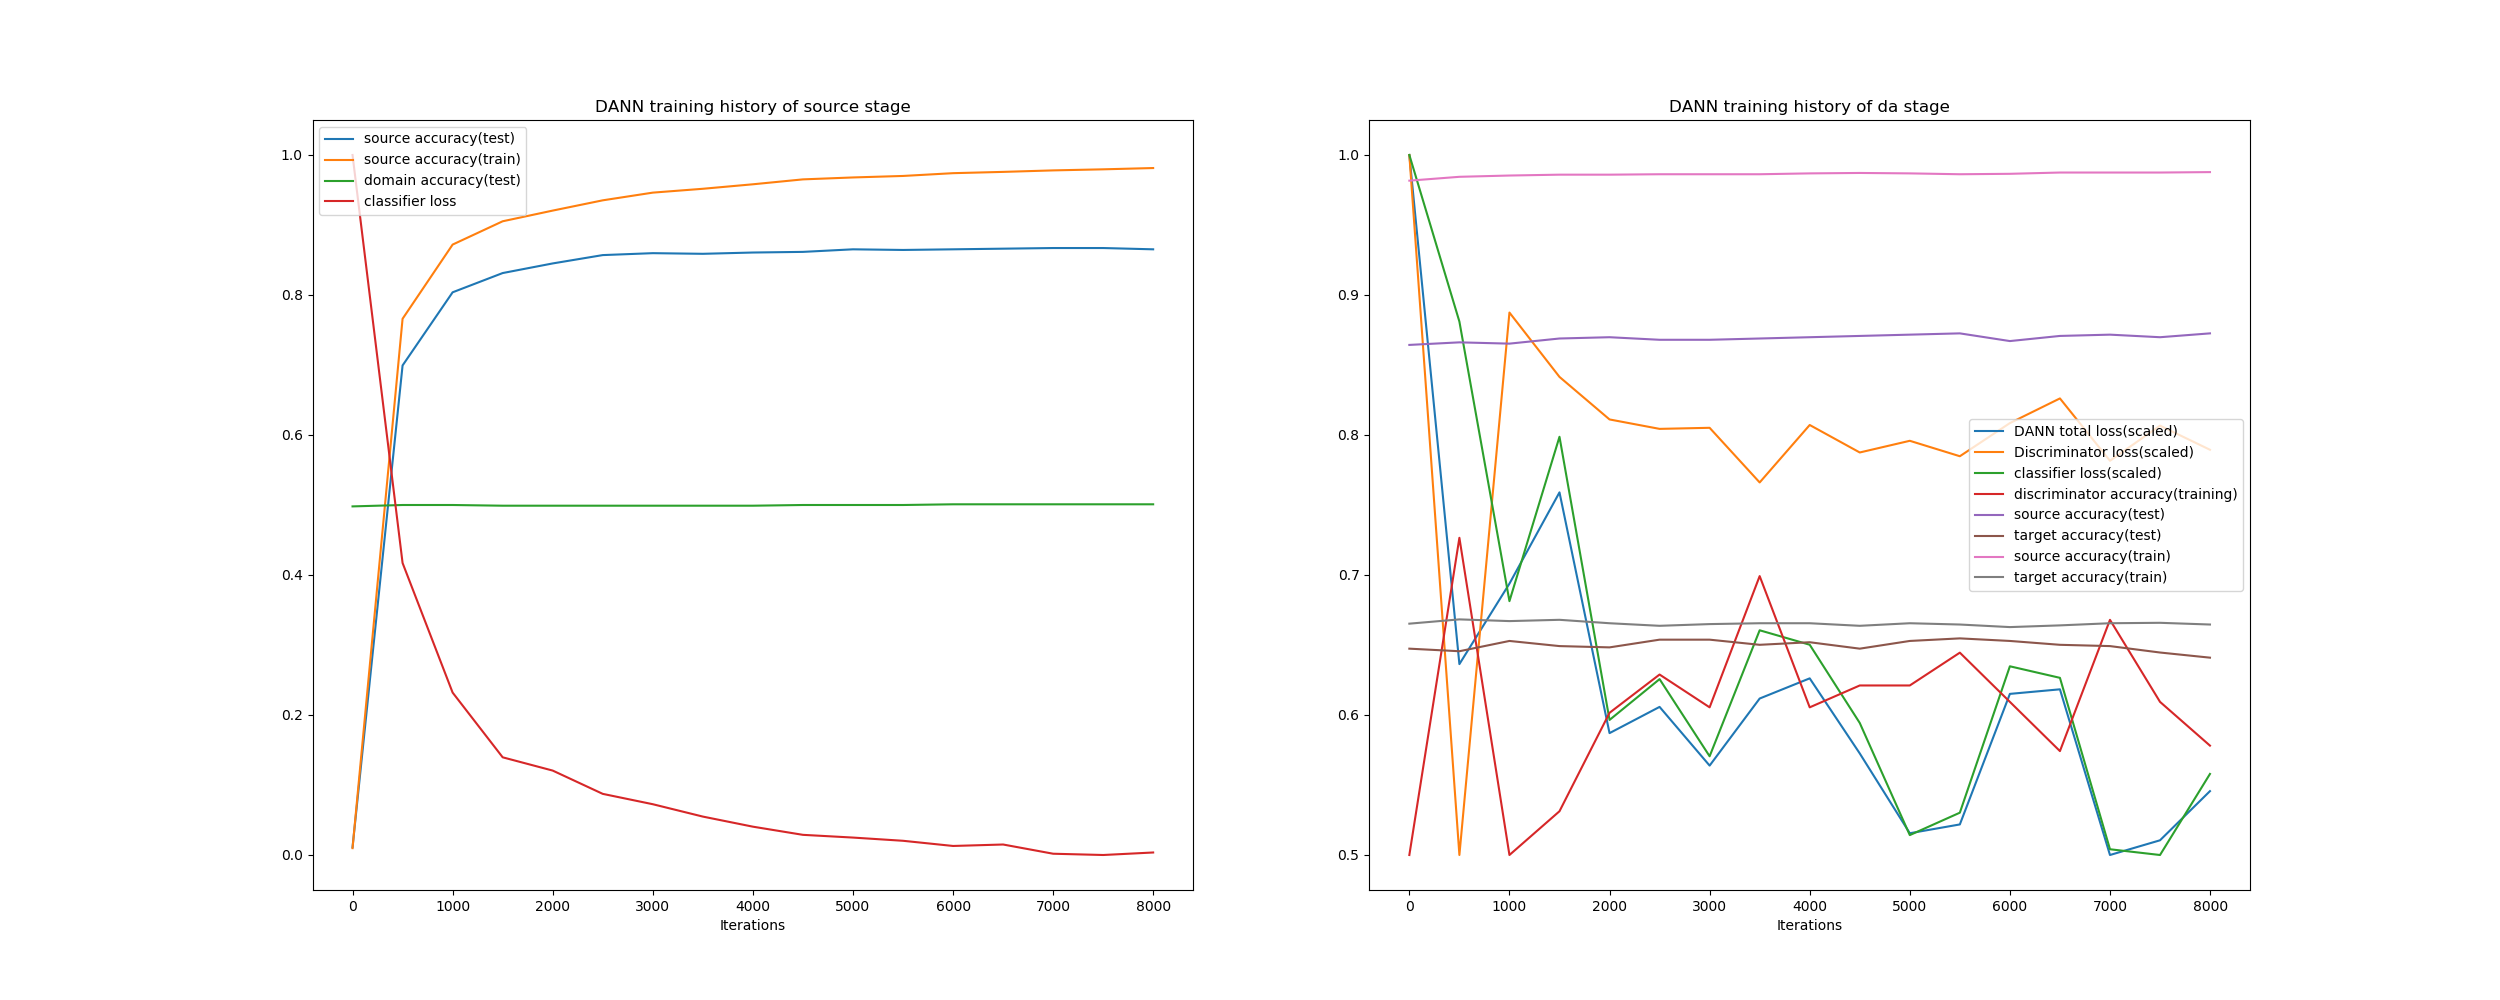
\includegraphics[width=3.5in, height=1.5in]{Ldann/std_C2R/dann.png}
\end{minipage}%
\caption{Visualization of DANN ExC Result}\label{fig:ExC2}
\end{figure*}

\begin{figure*}[htb]
\centering
\begin{minipage}[t]{0.26\textwidth}
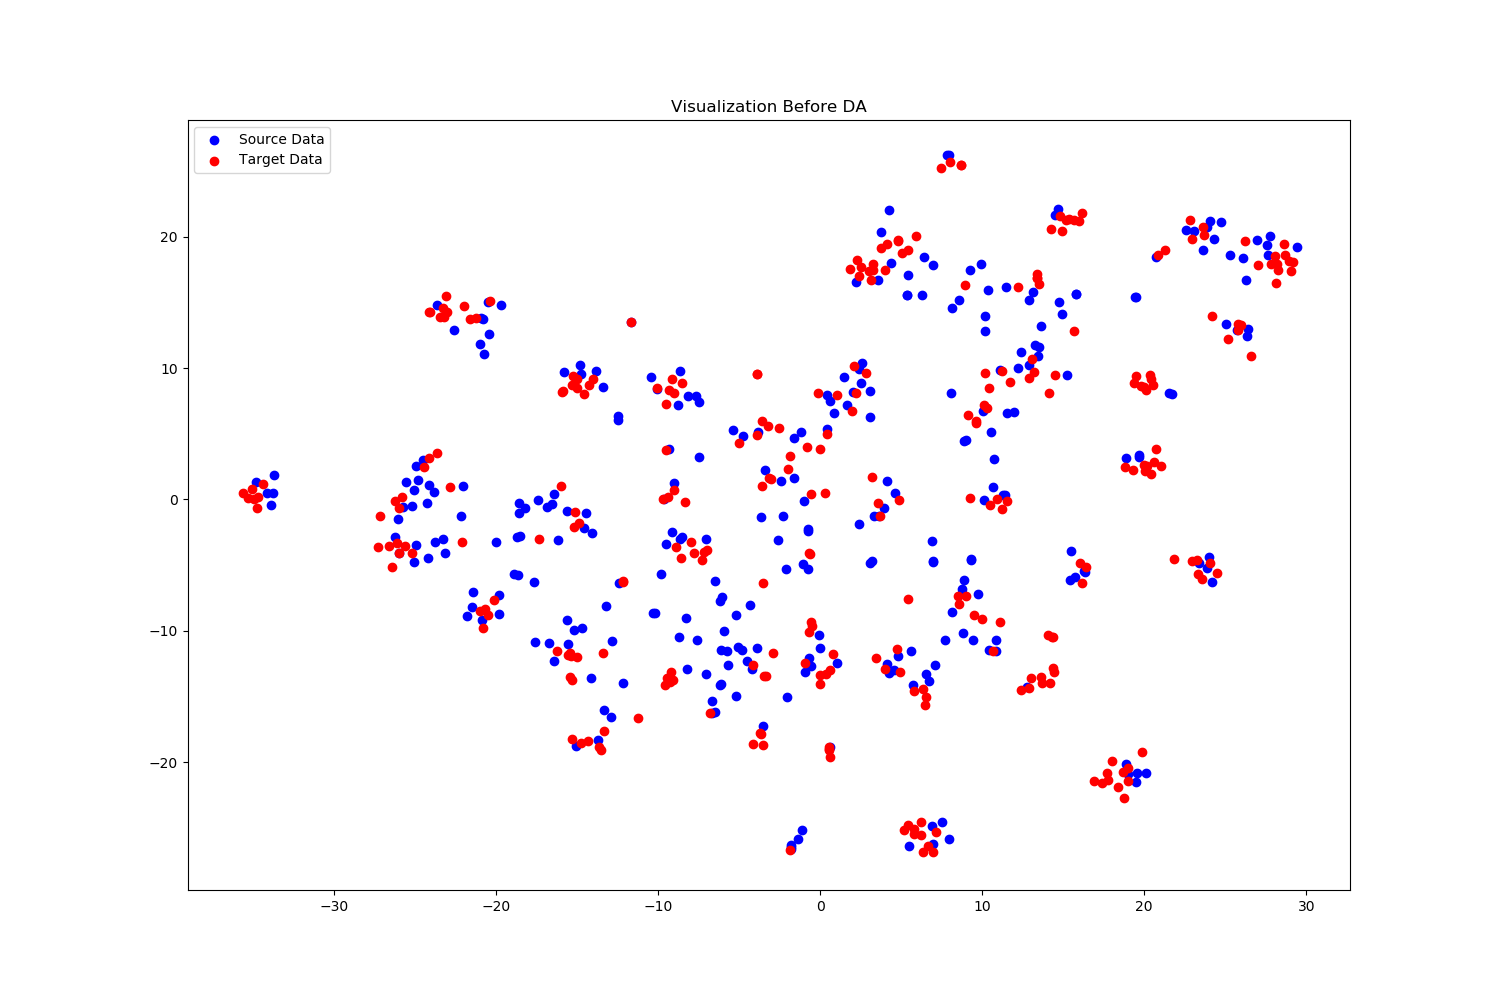
\includegraphics[width=1.6in, height=1.5in]{Ldann/std_P2R/before.png}
\end{minipage}%
\begin{minipage}[t]{0.26\textwidth}
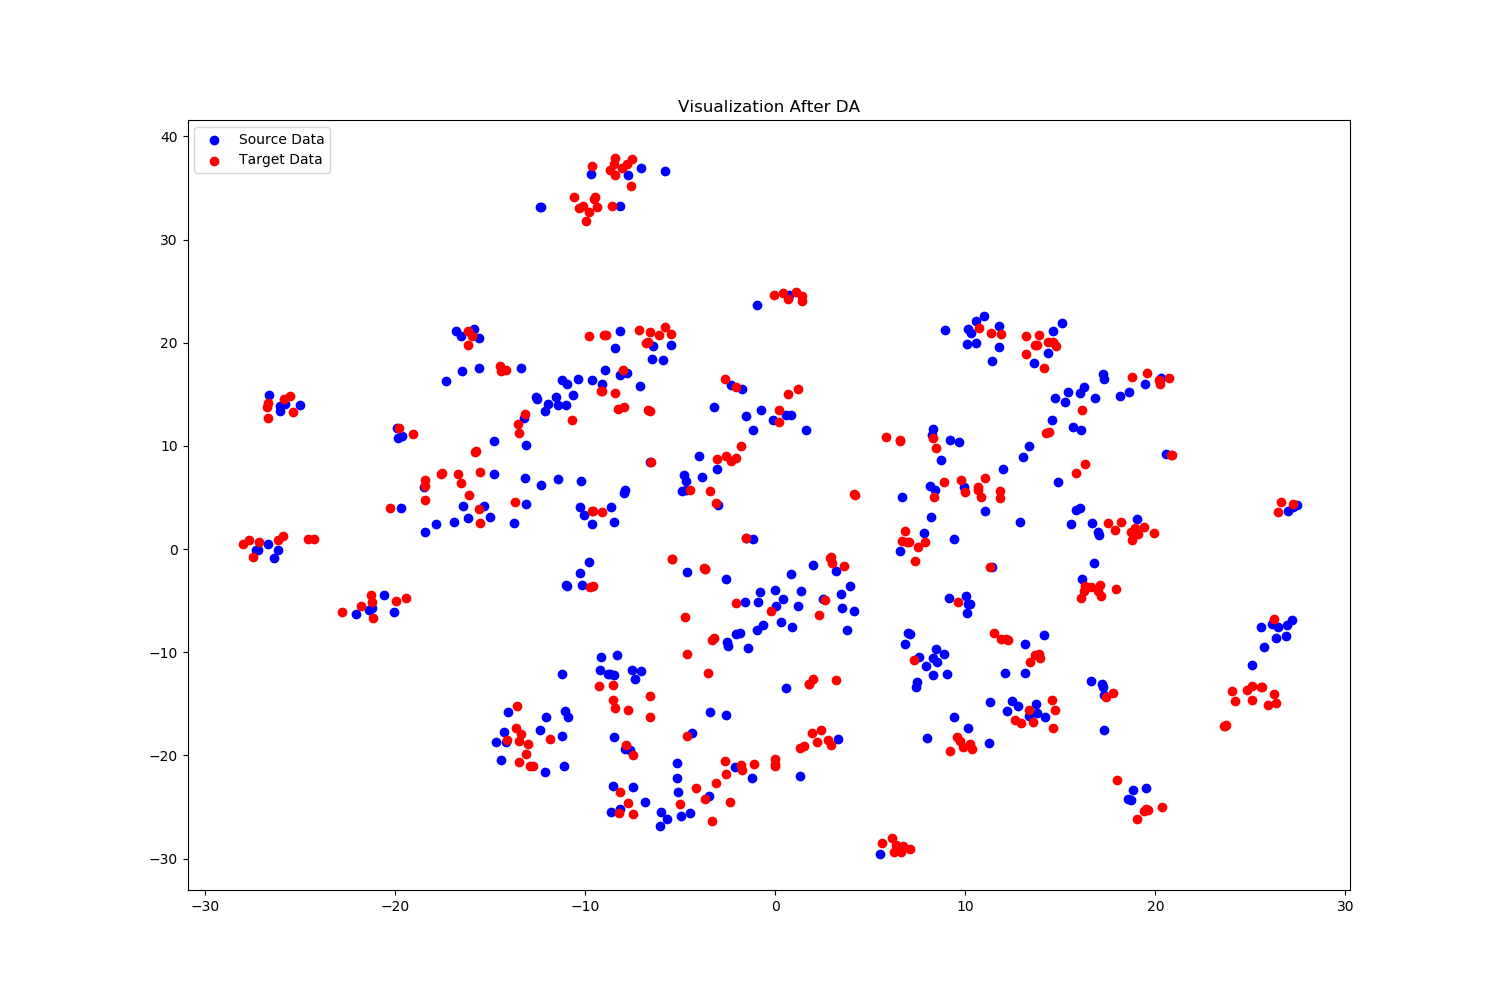
\includegraphics[width=1.6in, height=1.5in]{Ldann/std_P2R/after.png}
\end{minipage}%
\begin{minipage}[t]{0.45\textwidth}
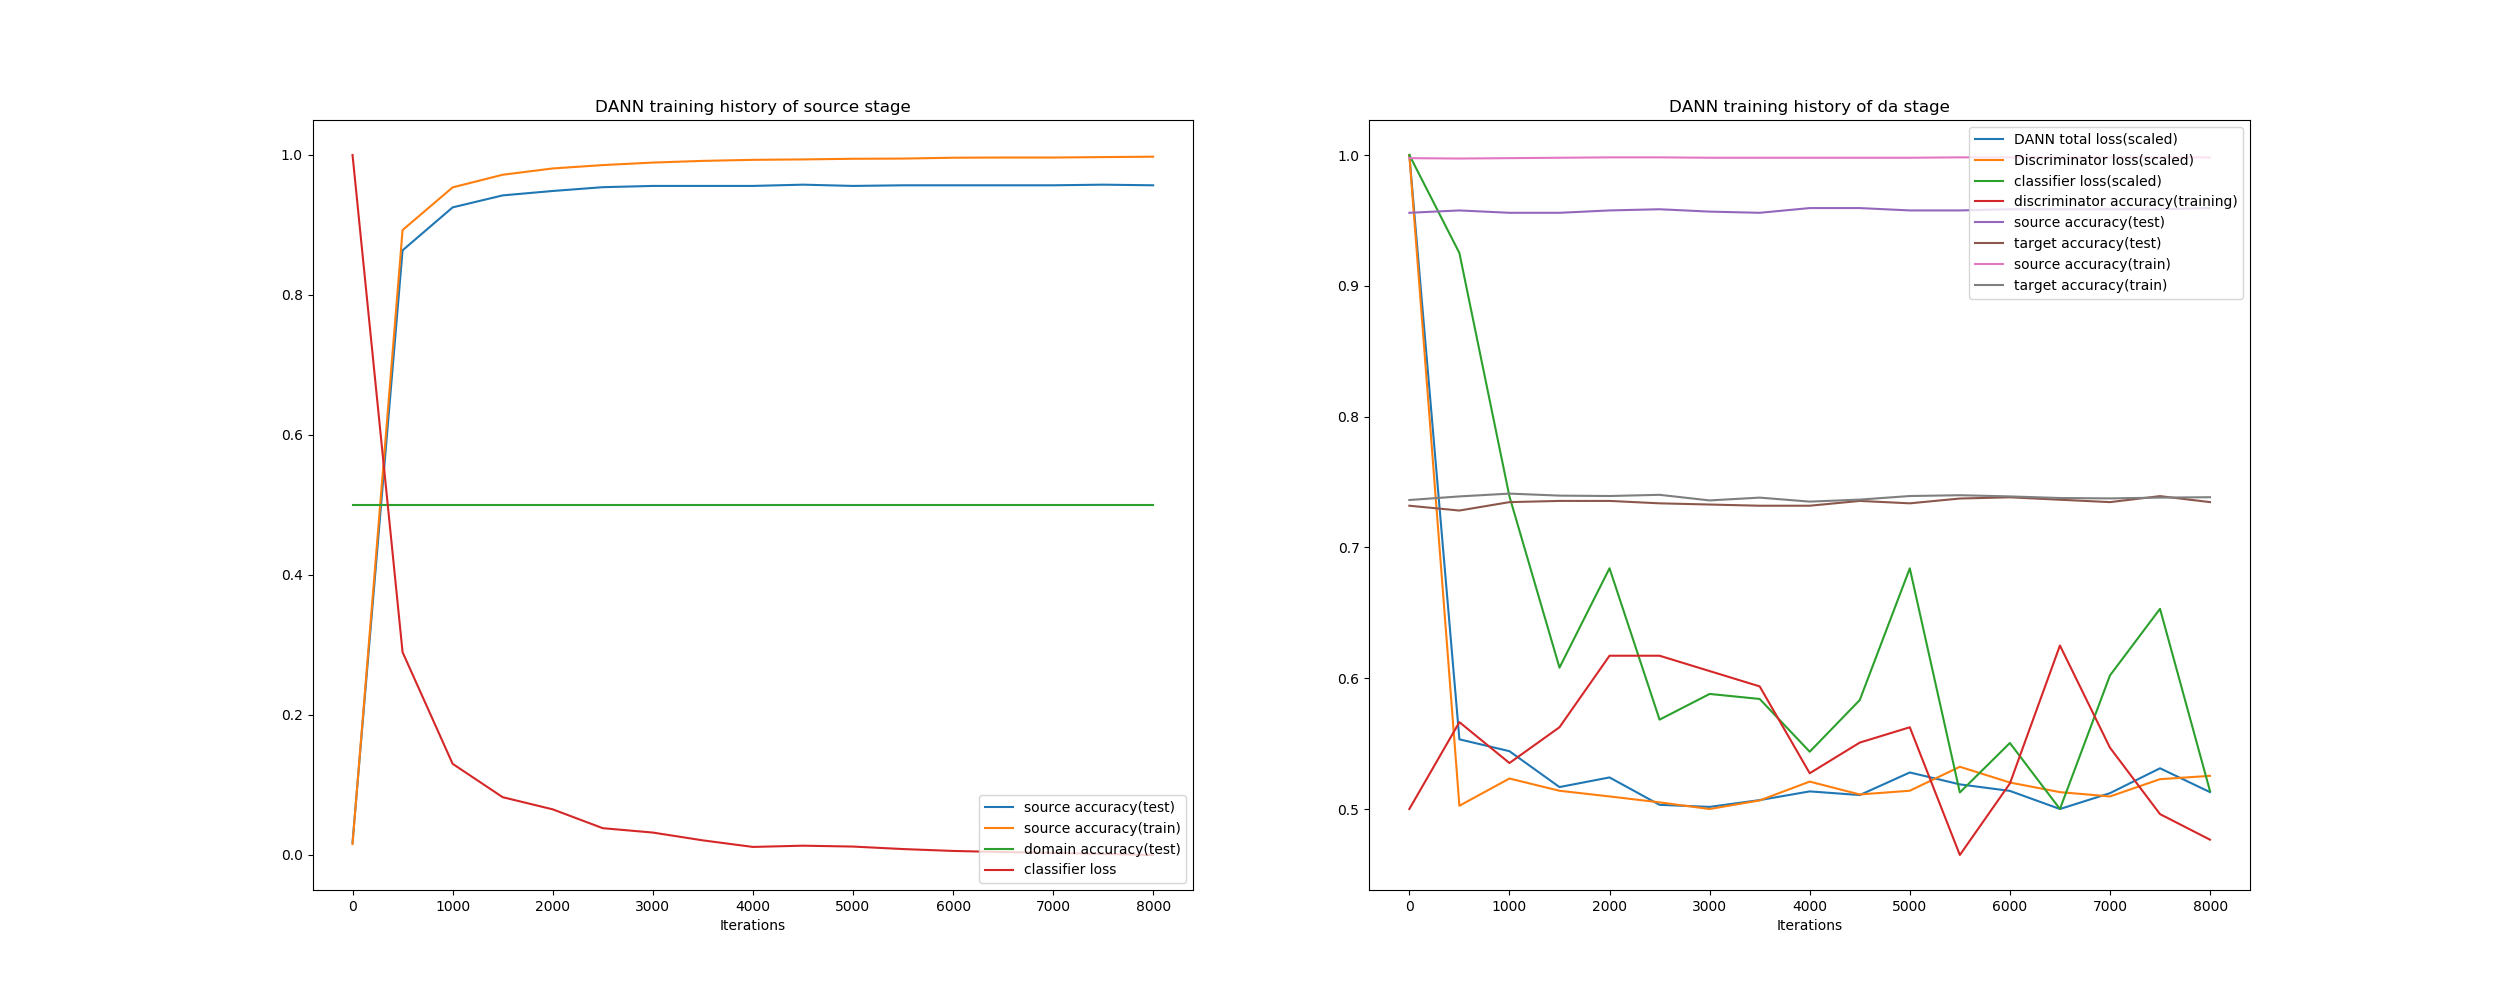
\includegraphics[width=3.5in, height=1.5in]{Ldann/std_P2R/dann.png}
\end{minipage}%
\caption{Visualization of DANN ExP Result}\label{fig:ExP2}
\end{figure*}

\end{document}





